\section{Background fractions and shapes in differential bins for \texorpdfstring{$\Zllll$}{Z to 4l} measurements}

\subsection{Background fractions} \label{app:z4l_bkginputs_fractions}

\begin{table}[!h!tb]  
\begin{center}  
\small  
    \caption{  
        Estimated fraction of background events in each bin of $\pt(4\ell)$, for Z$\to$4l measurements, for each final state.  
\label{tab:z4l_fractions_pT4l}  
}  
\begin{tabular}{|l|c|c|c|c|c|}  
\hline  
Background & final state & $0\leq$$\pt(4\ell)$$<15$ & $15\leq$$\pt(4\ell)$$<30$ & $30\leq$$\pt(4\ell)$$<60$ & $60\leq$$\pt(4\ell)$$<200$ \\ \hline 
qqZZ& $4e$  & 0.445 & 0.274 & 0.19 & 0.091  \\
qqZZ& $4\mu$  & 0.522 & 0.24 & 0.178 & 0.057  \\
qqZZ& $2e2\mu$  & 0.612 & 0.204 & 0.15 & 0.034  \\
ggZZ& $4e$  & 0.354 & 0.271 & 0.248 & 0.127  \\
ggZZ& $4\mu$  & 0.36 & 0.282 & 0.244 & 0.114  \\
ggZZ& $2e2\mu$  & 0.347 & 0.276 & 0.252 & 0.124  \\
Z+X (CR)& $4l$  & 0.208 & 0.316 & 0.342 & 0.134  \\
\hline  
\end{tabular}  
\normalsize  
\end{center}  
\end{table}  

\begin{table}[!h!tb]  
\begin{center}  
\small  
    \caption{  
        Estimated fraction of background events in each bin of $m(\mathrm{Z}_{2})$, for Z$\to$4l measurements, for each final state.  
\label{tab:z4l_fractions_massZ2}  
}  
\begin{tabular}{|l|c|c|c|c|c|}  
\hline  
Background & final state & $12\leq$$m(\mathrm{Z}_{2})$$<20$ & $20\leq$$m(\mathrm{Z}_{2})$$<28$ & $28\leq$$m(\mathrm{Z}_{2})$$<35$ & $35\leq$$m(\mathrm{Z}_{2})$$<120$ \\ \hline  
qqZZ& $4e$  & 0.318 & 0.303 & 0.23 & 0.15  \\
qqZZ& $4\mu$  & 0.548 & 0.256 & 0.11 & 0.085  \\
qqZZ& $2e2\mu$  & 0.689 & 0.194 & 0.049 & 0.068  \\
ggZZ& $4e$  & 0.153 & 0.223 & 0.251 & 0.373  \\
ggZZ& $4\mu$  & 0.212 & 0.264 & 0.218 & 0.306  \\
ggZZ& $2e2\mu$  & 0.397 & 0.269 & 0.167 & 0.167  \\
Z+X (CR)& $4l$  & 0.443 & 0.365 & 0.113 & 0.079  \\
\hline  
\end{tabular}  
\normalsize  
\end{center}  
\end{table}  

\begin{table}[!h!tb]  
\begin{center}  
\small  
    \caption{  
        Estimated fraction of background events in each bin of $N_{\rm jets}$, for Z$\to$4l measurements, for each final state.  
\label{tab:z4l_fractions_njets_reco_pt30_eta4p7}  
}  
\begin{tabular}{|l|c|c|c|c|c|}  
\hline  
Background & final state & $0\leq$$N_{\rm jets}$$<1$ & $1\leq$$N_{\rm jets}$$<2$ & $2\leq$$N_{\rm jets}$$<3$ & $3\leq$$N_{\rm jets}$$<10$ \\ \hline  
qqZZ& $4e$  & 0.752 & 0.204 & 0.036 & 0.007  \\
qqZZ& $4\mu$  & 0.775 & 0.194 & 0.027 & 0.004  \\
qqZZ& $2e2\mu$  & 0.845 & 0.131 & 0.019 & 0.005  \\
ggZZ& $4e$  & 0.666 & 0.266 & 0.058 & 0.01  \\
ggZZ& $4\mu$  & 0.693 & 0.25 & 0.05 & 0.008  \\
ggZZ& $2e2\mu$  & 0.676 & 0.255 & 0.059 & 0.01  \\
Z+X (CR)& $4l$  & 0.596 & 0.259 & 0.102 & 0.044  \\
\hline  
\end{tabular}  
\normalsize  
\end{center}  
\end{table}  

\begin{table}[!h!tb]  
\begin{center}  
\small  
    \caption{  
        Estimated fraction of background events in each bin of $|y(4\ell)|$, for Z$\to$4l measurements, for each final state.  
\label{tab:z4l_fractions_rapidity4l}  
}  
\begin{tabular}{|l|c|c|c|c|c|}  
\hline  
Background & final state & $0\leq$$|y(4\ell)|$$<0.4$ & $0.4\leq$$|y(4\ell)|$$<0.8$ & $0.8\leq$$|y(4\ell)|$$<1.2$ & $1.2\leq$$|y(4\ell)|$$<2.4$ \\ \hline  
qqZZ& $4e$  & 0.263 & 0.285 & 0.212 & 0.237  \\
qqZZ& $4\mu$  & 0.245 & 0.238 & 0.239 & 0.278  \\
qqZZ& $2e2\mu$  & 0.218 & 0.238 & 0.248 & 0.296  \\
ggZZ& $4e$  & 0.333 & 0.29 & 0.212 & 0.164  \\
ggZZ& $4\mu$  & 0.31 & 0.275 & 0.22 & 0.194  \\
ggZZ& $2e2\mu$  & 0.326 & 0.298 & 0.215 & 0.161  \\
Z+X (CR)& $4l$  & 0.21 & 0.261 & 0.259 & 0.27  \\
\hline  
\end{tabular}  
\normalsize  
\end{center}  
\end{table}  

\begin{table}[!h!tb]  
\begin{center}  
\small  
    \caption{  
        Estimated fraction of background events in each bin of $|\cos \theta^{*}|$, for Z$\to$4l measurements, for each final state.  
\label{tab:z4l_fractions_cosThetaStar}  
}  
\begin{tabular}{|l|c|c|c|c|c|}  
\hline  
Background & final state & $0.0\leq$$|\cos \theta^{*}|$$<0.25$ & $0.25\leq$$|\cos \theta^{*}|$$<0.5$ & $0.5\leq$$|\cos \theta^{*}|$$<0.75$ & $0.75\leq$$|\cos \theta^{*}|$$<1.0$ \\ \hline  
qqZZ& $4e$  & 0.27 & 0.285 & 0.234 & 0.212  \\
qqZZ& $4\mu$  & 0.27 & 0.216 & 0.231 & 0.282  \\
qqZZ& $2e2\mu$  & 0.233 & 0.175 & 0.238 & 0.354  \\
ggZZ& $4e$  & 0.257 & 0.262 & 0.26 & 0.221  \\
ggZZ& $4\mu$  & 0.249 & 0.262 & 0.257 & 0.231  \\
ggZZ& $2e2\mu$  & 0.217 & 0.218 & 0.245 & 0.32  \\
Z+X (CR)& $4l$  & 0.238 & 0.203 & 0.24 & 0.319  \\
\hline  
\end{tabular}  
\normalsize  
\end{center}  
\end{table} 

 \clearpage


\subsection{Background shapes in bins of $\pt(4\ell)$ } \label{app:z4l_bkginputs_shapes}

\begin{figure}[!ht]
  \begin{center}
  
    \subfigure[$0.0 \GeV < \pt(4\ell) < 15.0 \GeV$]{
      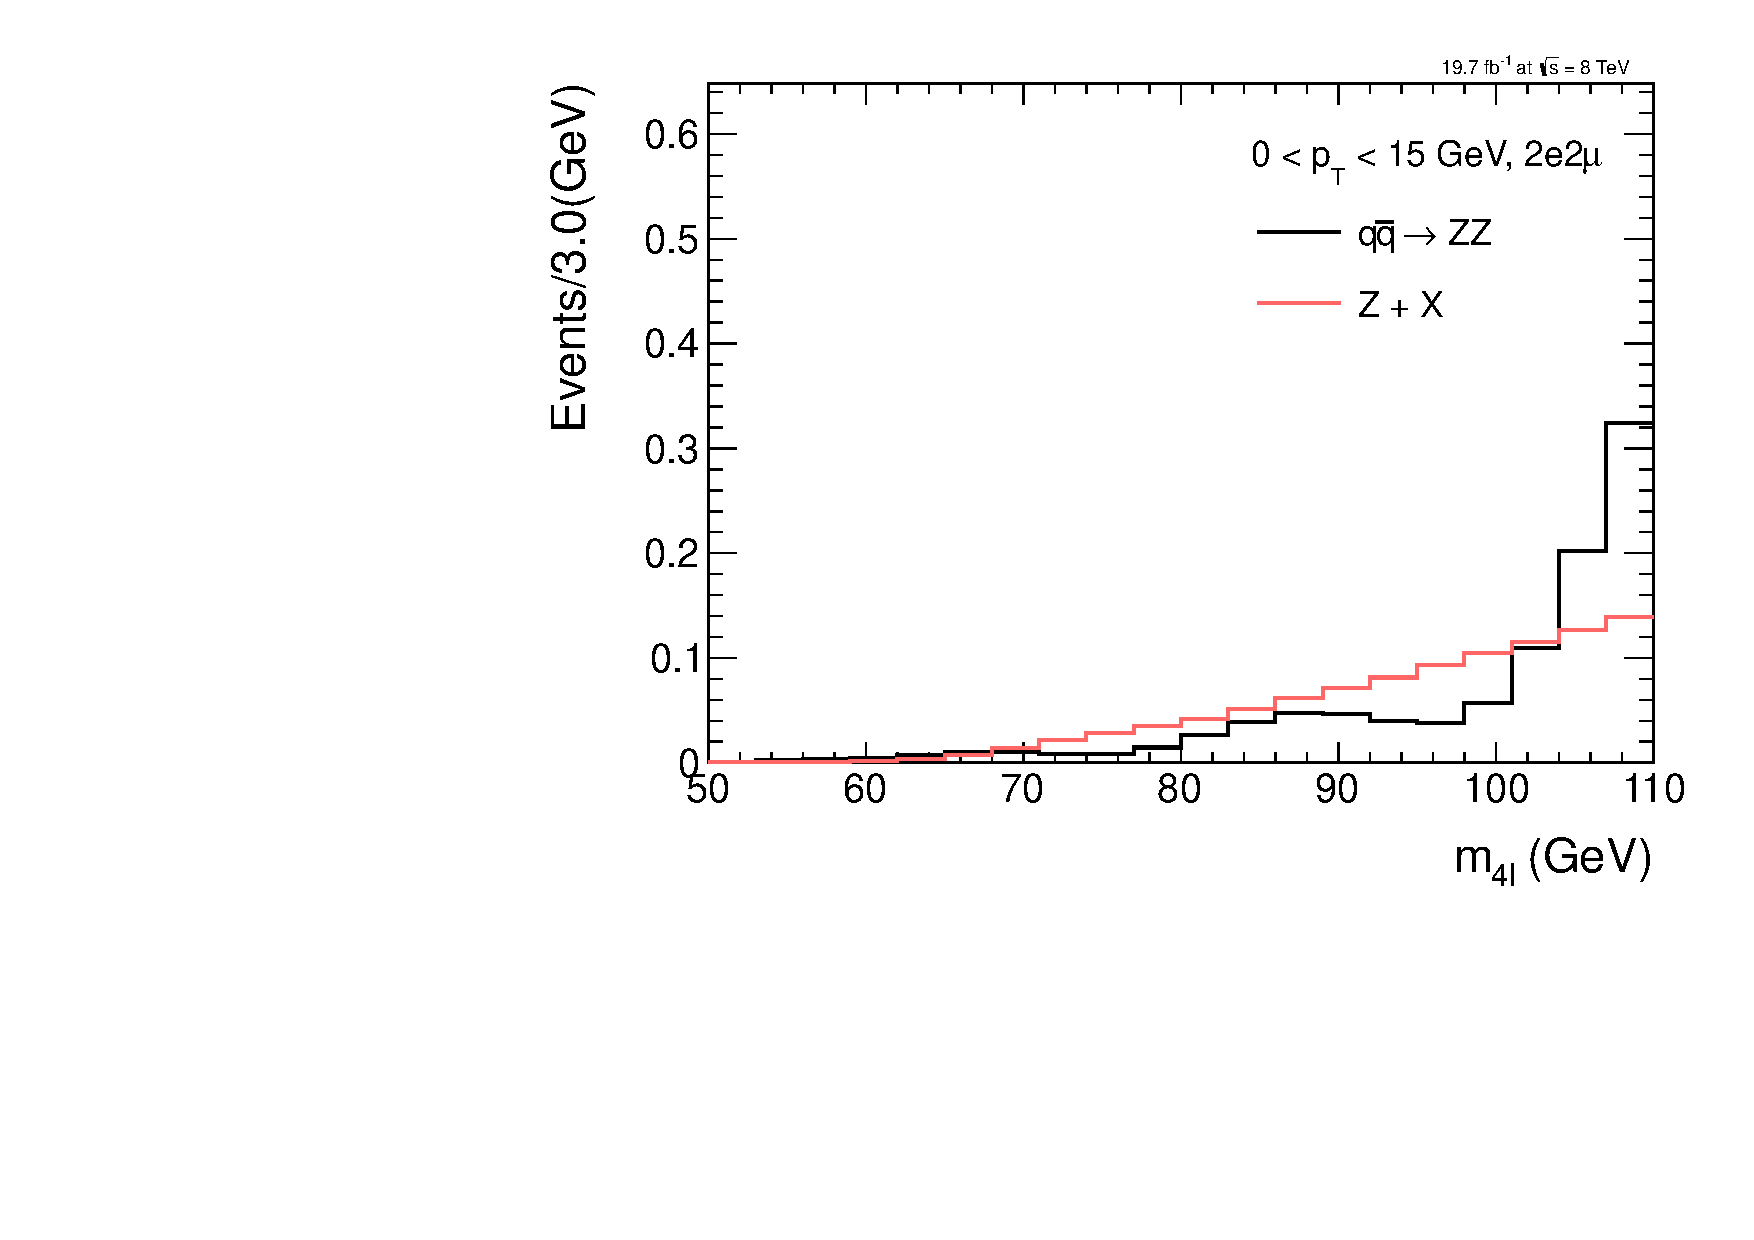
\includegraphics[width=0.32\textwidth,angle=0]{Appendix/figuresZ4l/XSTemplates_2e2mu_pT4l_0_15_qqZZ_ZJetsCR.pdf}
      \label{fig:z4l_bkg-pT4l-qqZZ-ZX-2e2mu:a}
    }    
    \subfigure[$0.0 \GeV < \pt(4\ell) < 15.0 \GeV$]{
      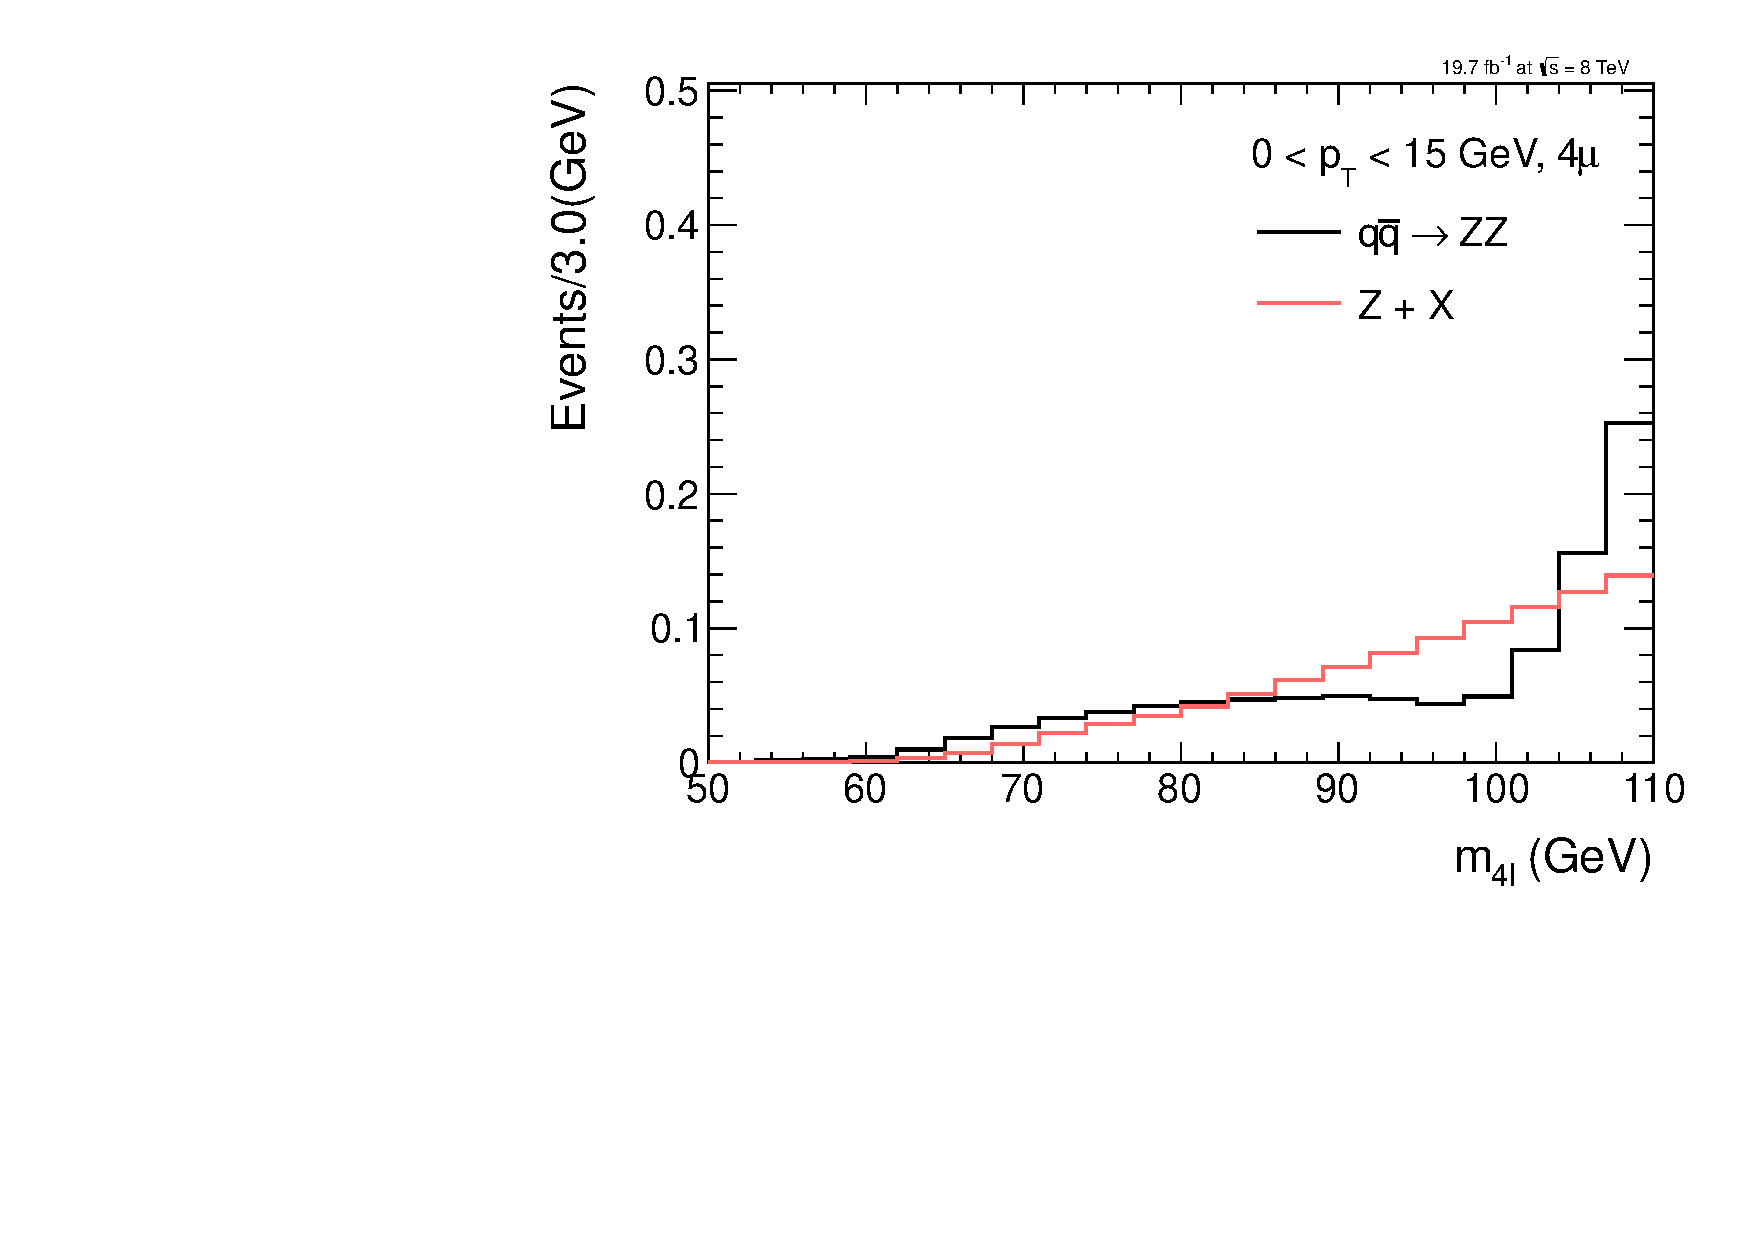
\includegraphics[width=0.32\textwidth,angle=0]{Appendix/figuresZ4l/XSTemplates_4mu_pT4l_0_15_qqZZ_ZJetsCR.pdf}
      \label{fig:z4l_bkg-pT4l-qqZZ-ZX-4mu:a}
    }    
    \subfigure[$0.0 \GeV < \pt(4\ell) < 15.0 \GeV$]{
      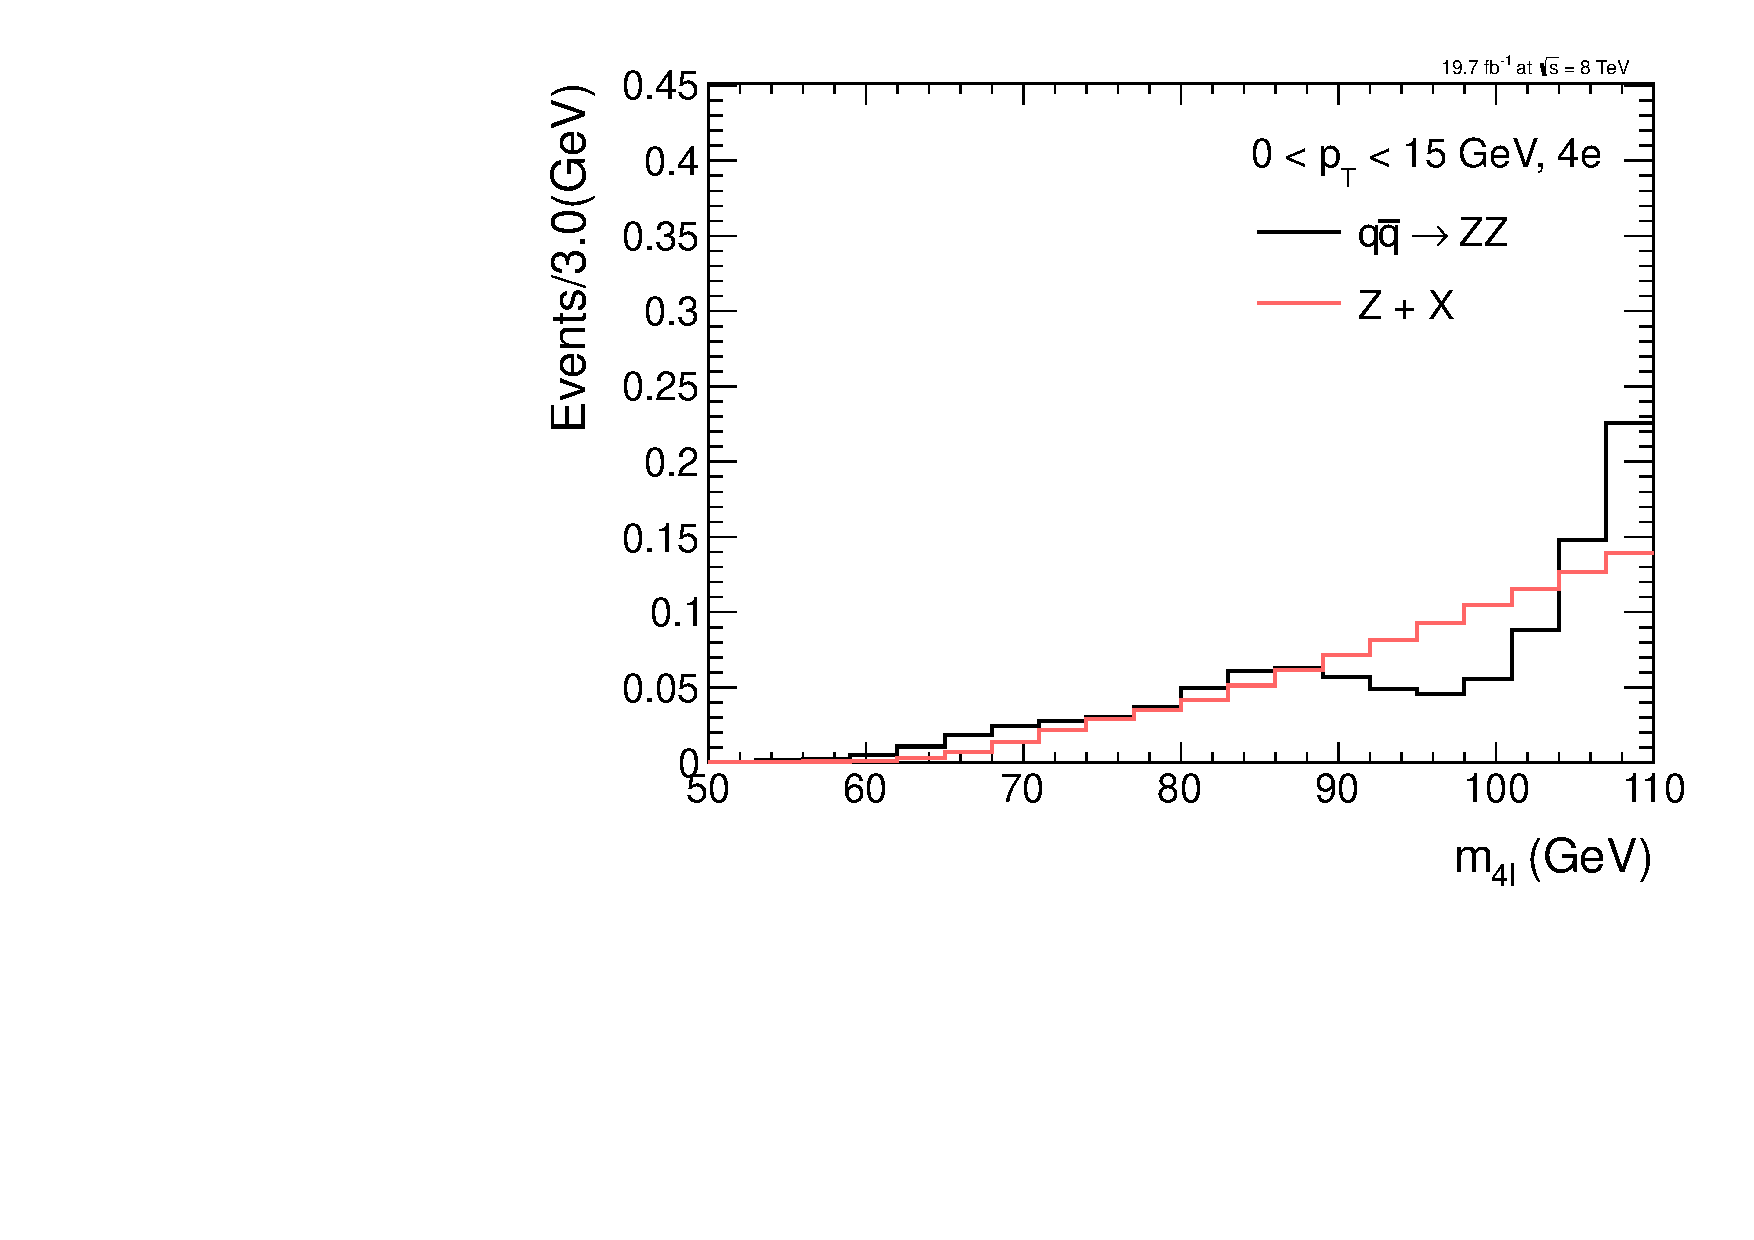
\includegraphics[width=0.32\textwidth,angle=0]{Appendix/figuresZ4l/XSTemplates_4e_pT4l_0_15_qqZZ_ZJetsCR.pdf}
      \label{fig:z4l_bkg-pT4l-qqZZ-ZX-4e:a}
    }    \\

    \subfigure[$15.0 \GeV < \pt(4\ell) < 30.0 \GeV$]{
      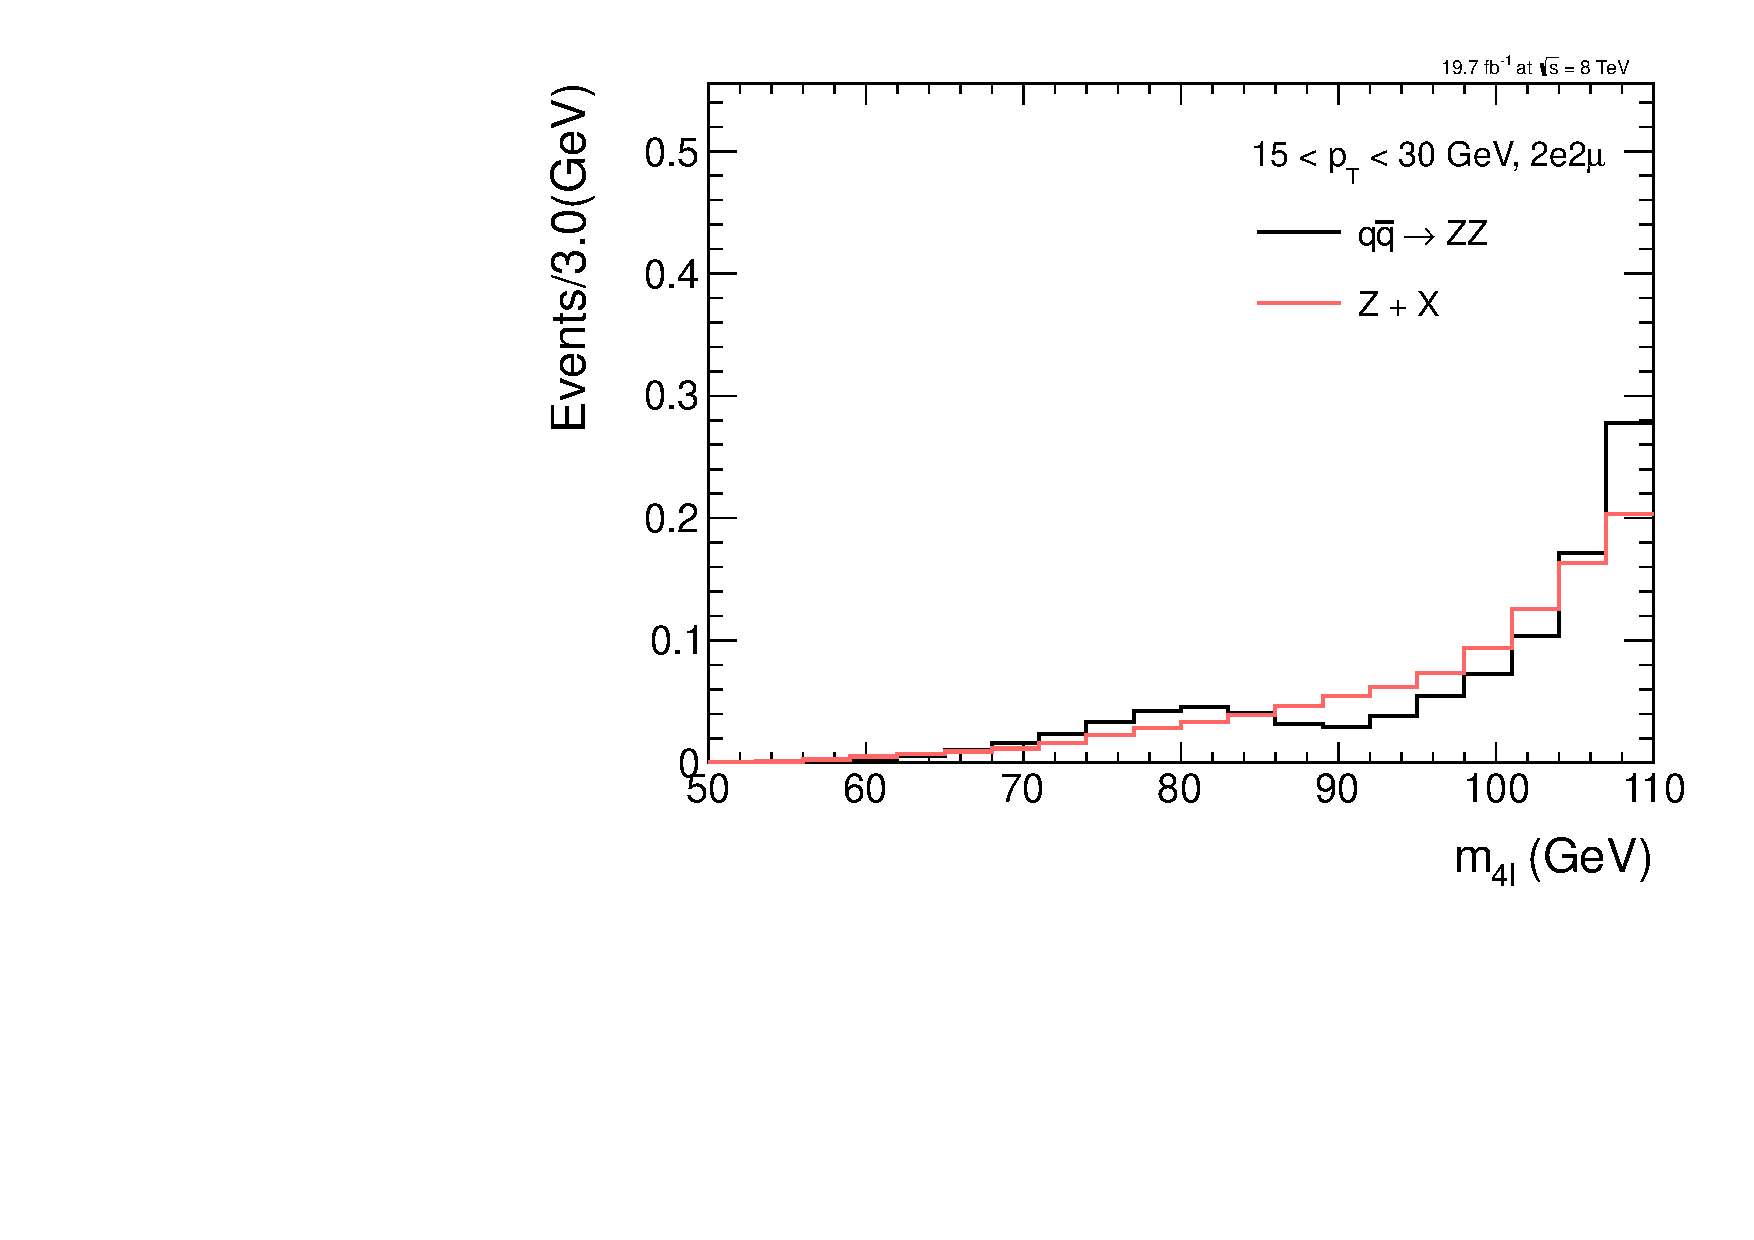
\includegraphics[width=0.32\textwidth,angle=0]{Appendix/figuresZ4l/XSTemplates_2e2mu_pT4l_15_30_qqZZ_ZJetsCR.pdf}
      \label{fig:z4l_bkg-pT4l-qqZZ-ZX-2e2mu:b}
    }
    \subfigure[$15.0 \GeV < \pt(4\ell) < 30.0 \GeV$]{
      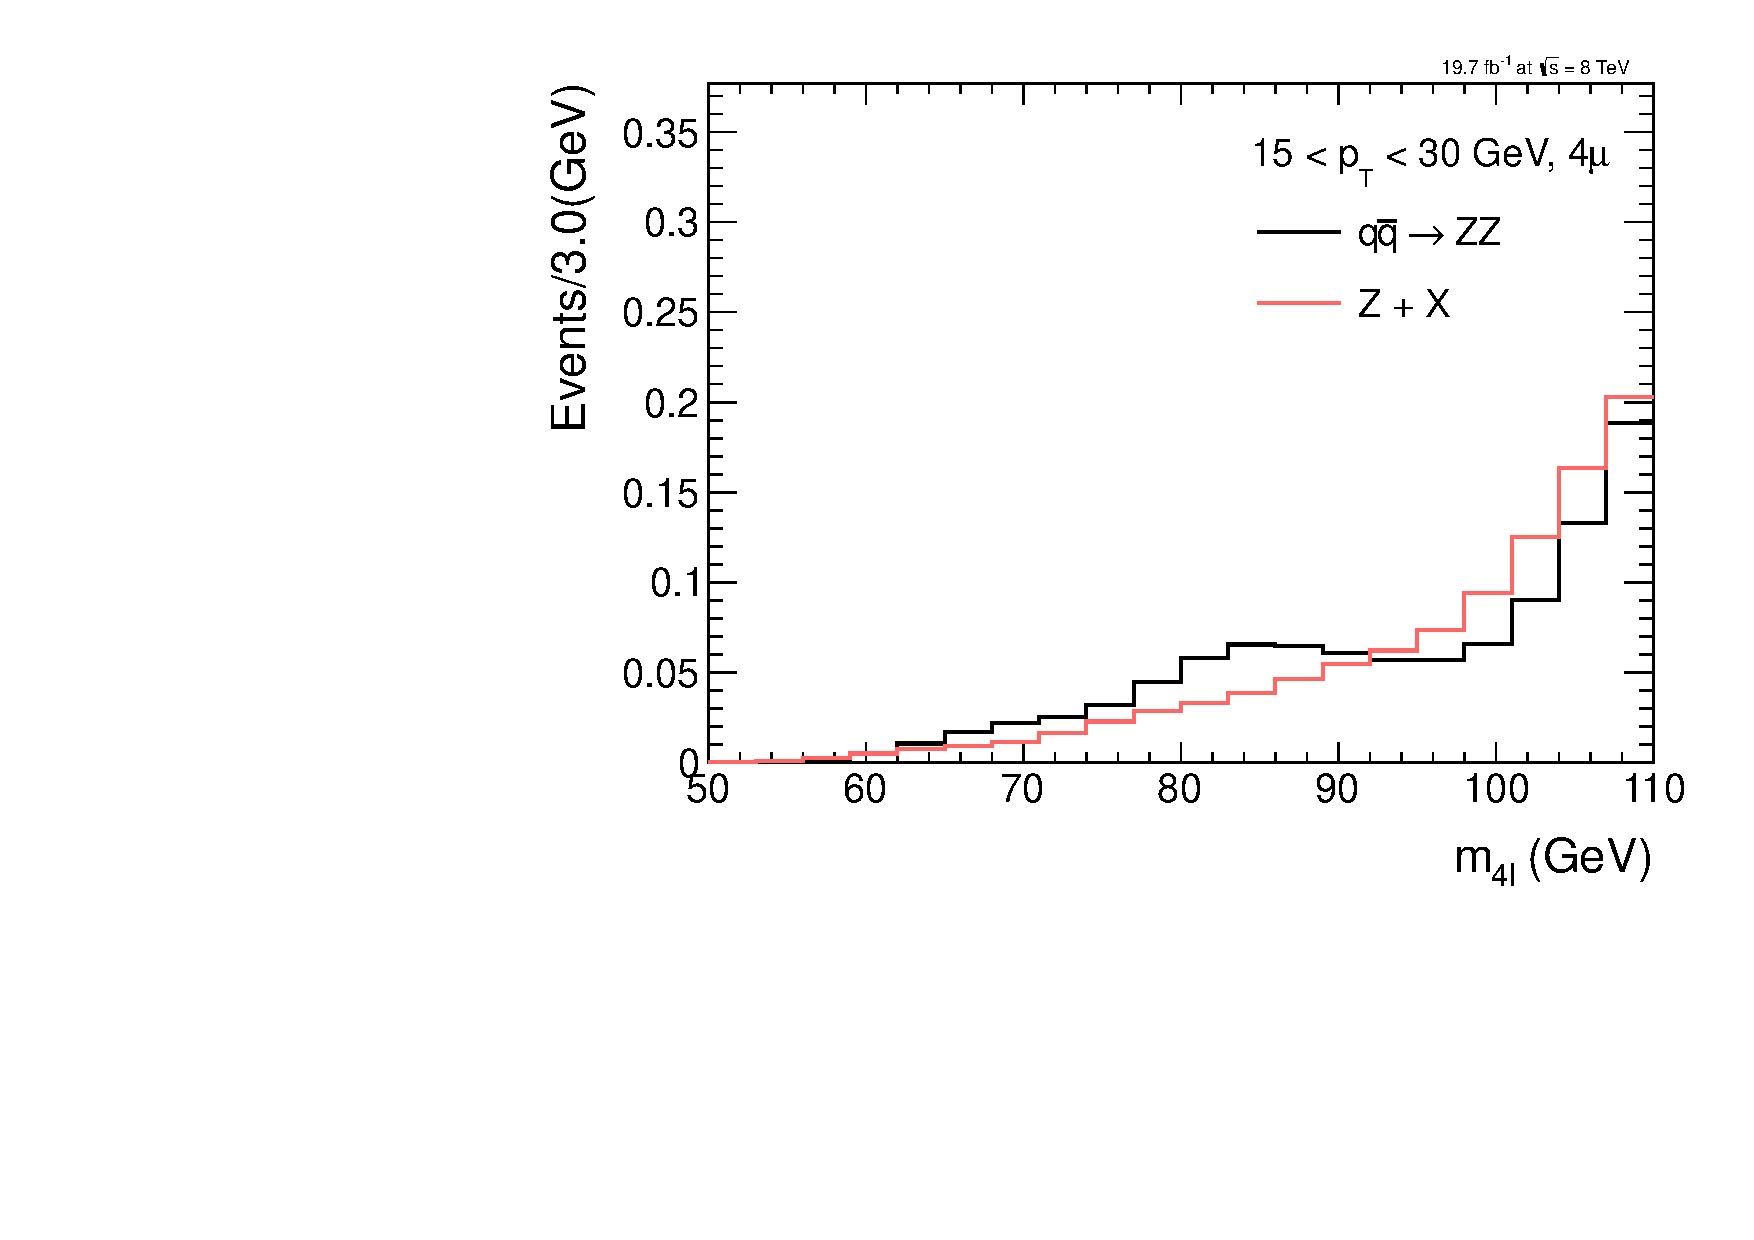
\includegraphics[width=0.32\textwidth,angle=0]{Appendix/figuresZ4l/XSTemplates_4mu_pT4l_15_30_qqZZ_ZJetsCR.pdf}
      \label{fig:z4l_bkg-pT4l-qqZZ-ZX-4mu:b}
    } 
    \subfigure[$15.0 \GeV < \pt(4\ell) < 30.0 \GeV$]{
      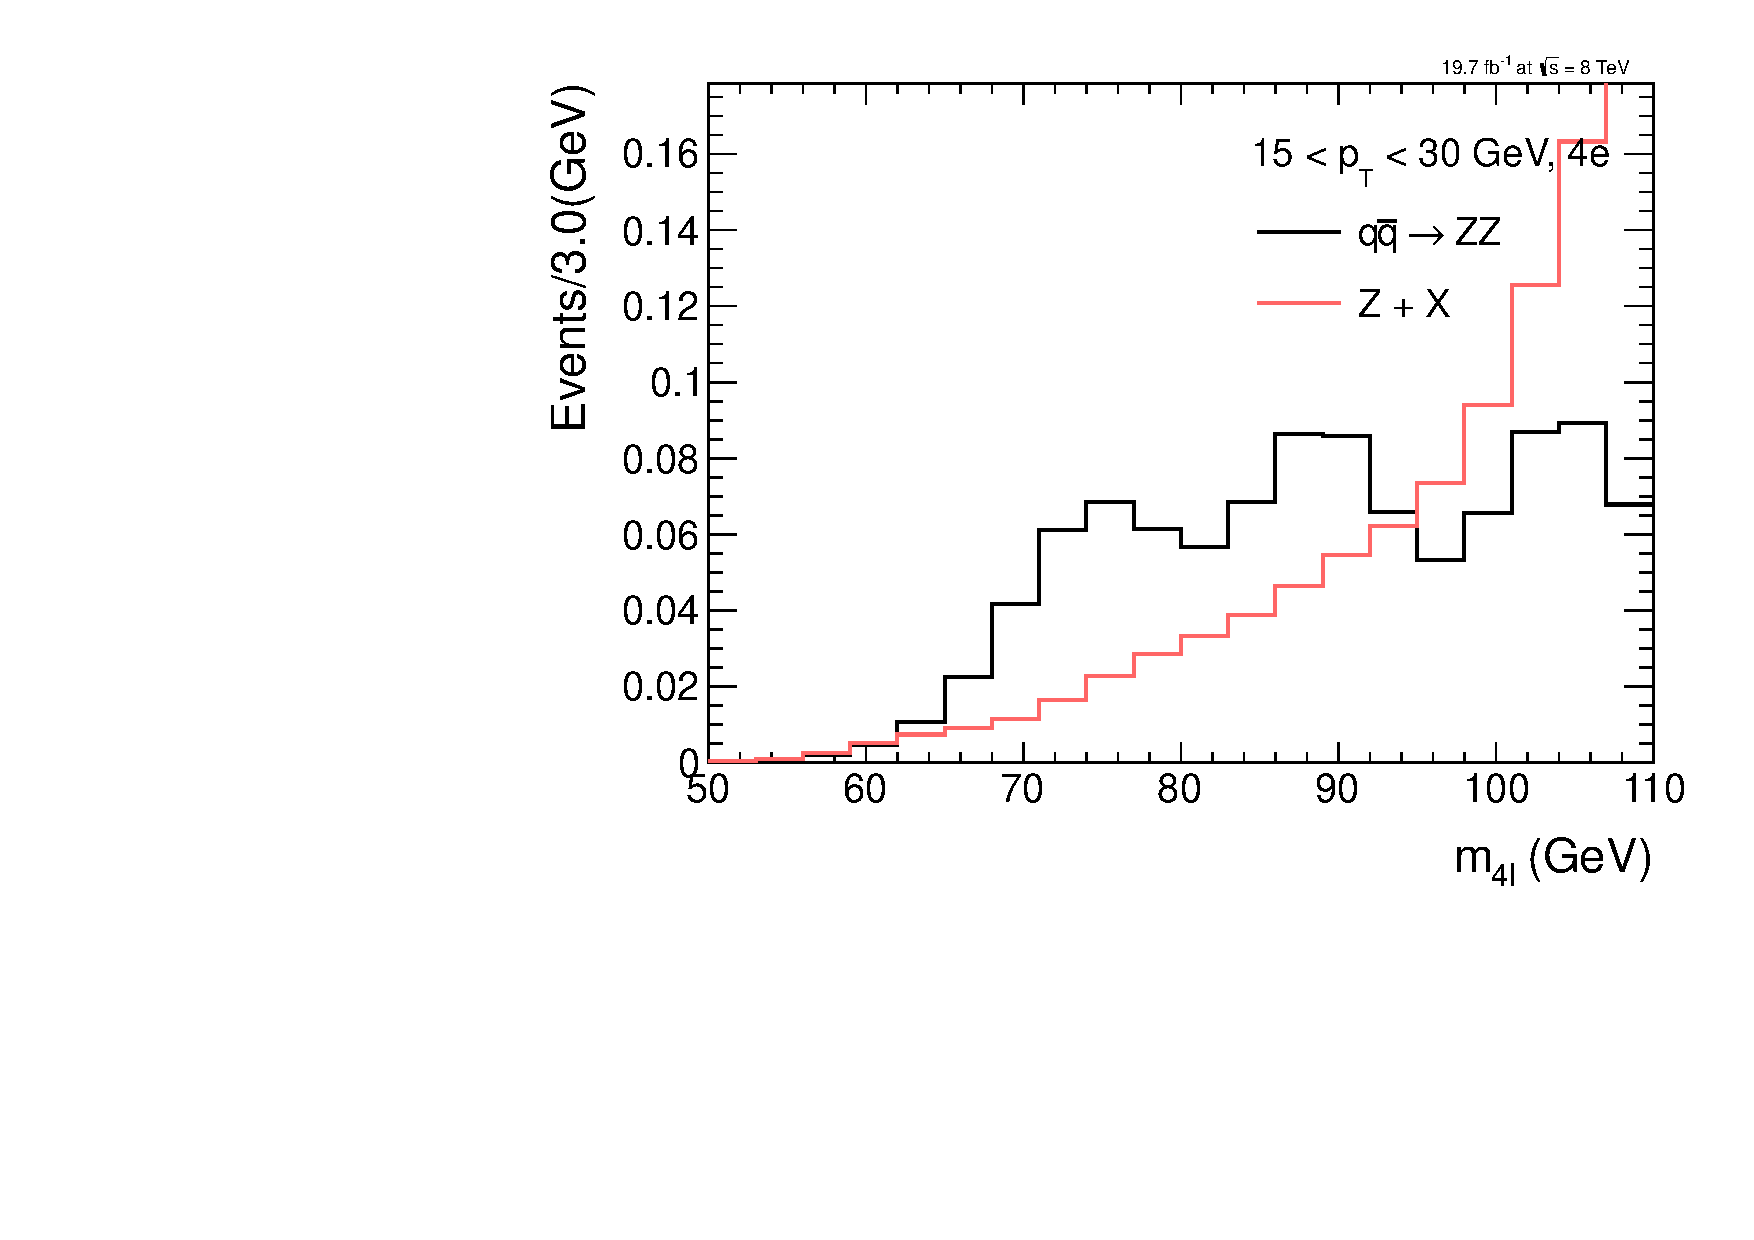
\includegraphics[width=0.32\textwidth,angle=0]{Appendix/figuresZ4l/XSTemplates_4e_pT4l_15_30_qqZZ_ZJetsCR.pdf}
      \label{fig:z4l_bkg-pT4l-qqZZ-ZX-4e:b}
    } \\
    
    \subfigure[$30.0 \GeV < \pt(4\ell) < 60.0 \GeV$]{
      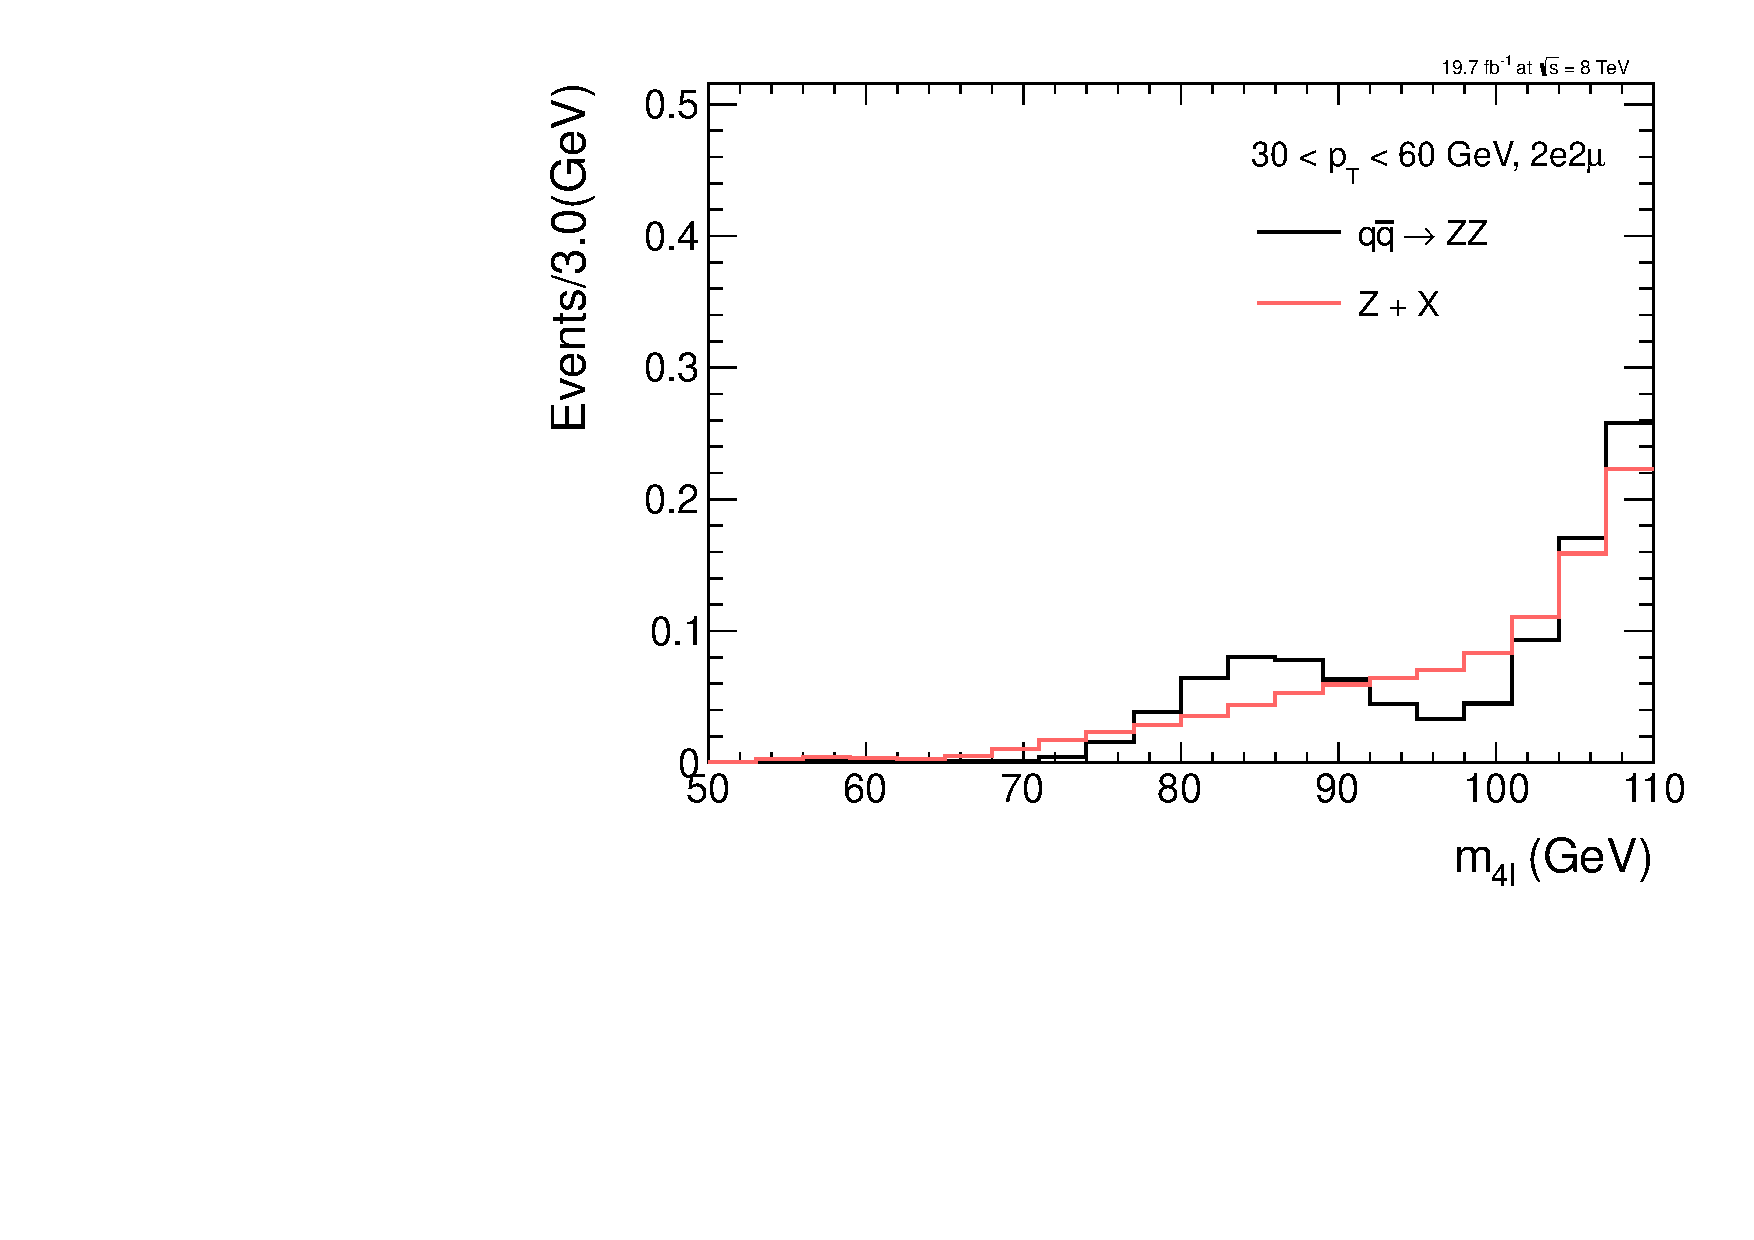
\includegraphics[width=0.32\textwidth,angle=0]{Appendix/figuresZ4l/XSTemplates_2e2mu_pT4l_30_60_qqZZ_ZJetsCR.pdf}
      \label{fig:z4l_bkg-pT4l-qqZZ-ZX-2e2mu:c}
    }
    \subfigure[$30.0 \GeV < \pt(4\ell) < 60.0 \GeV$]{
      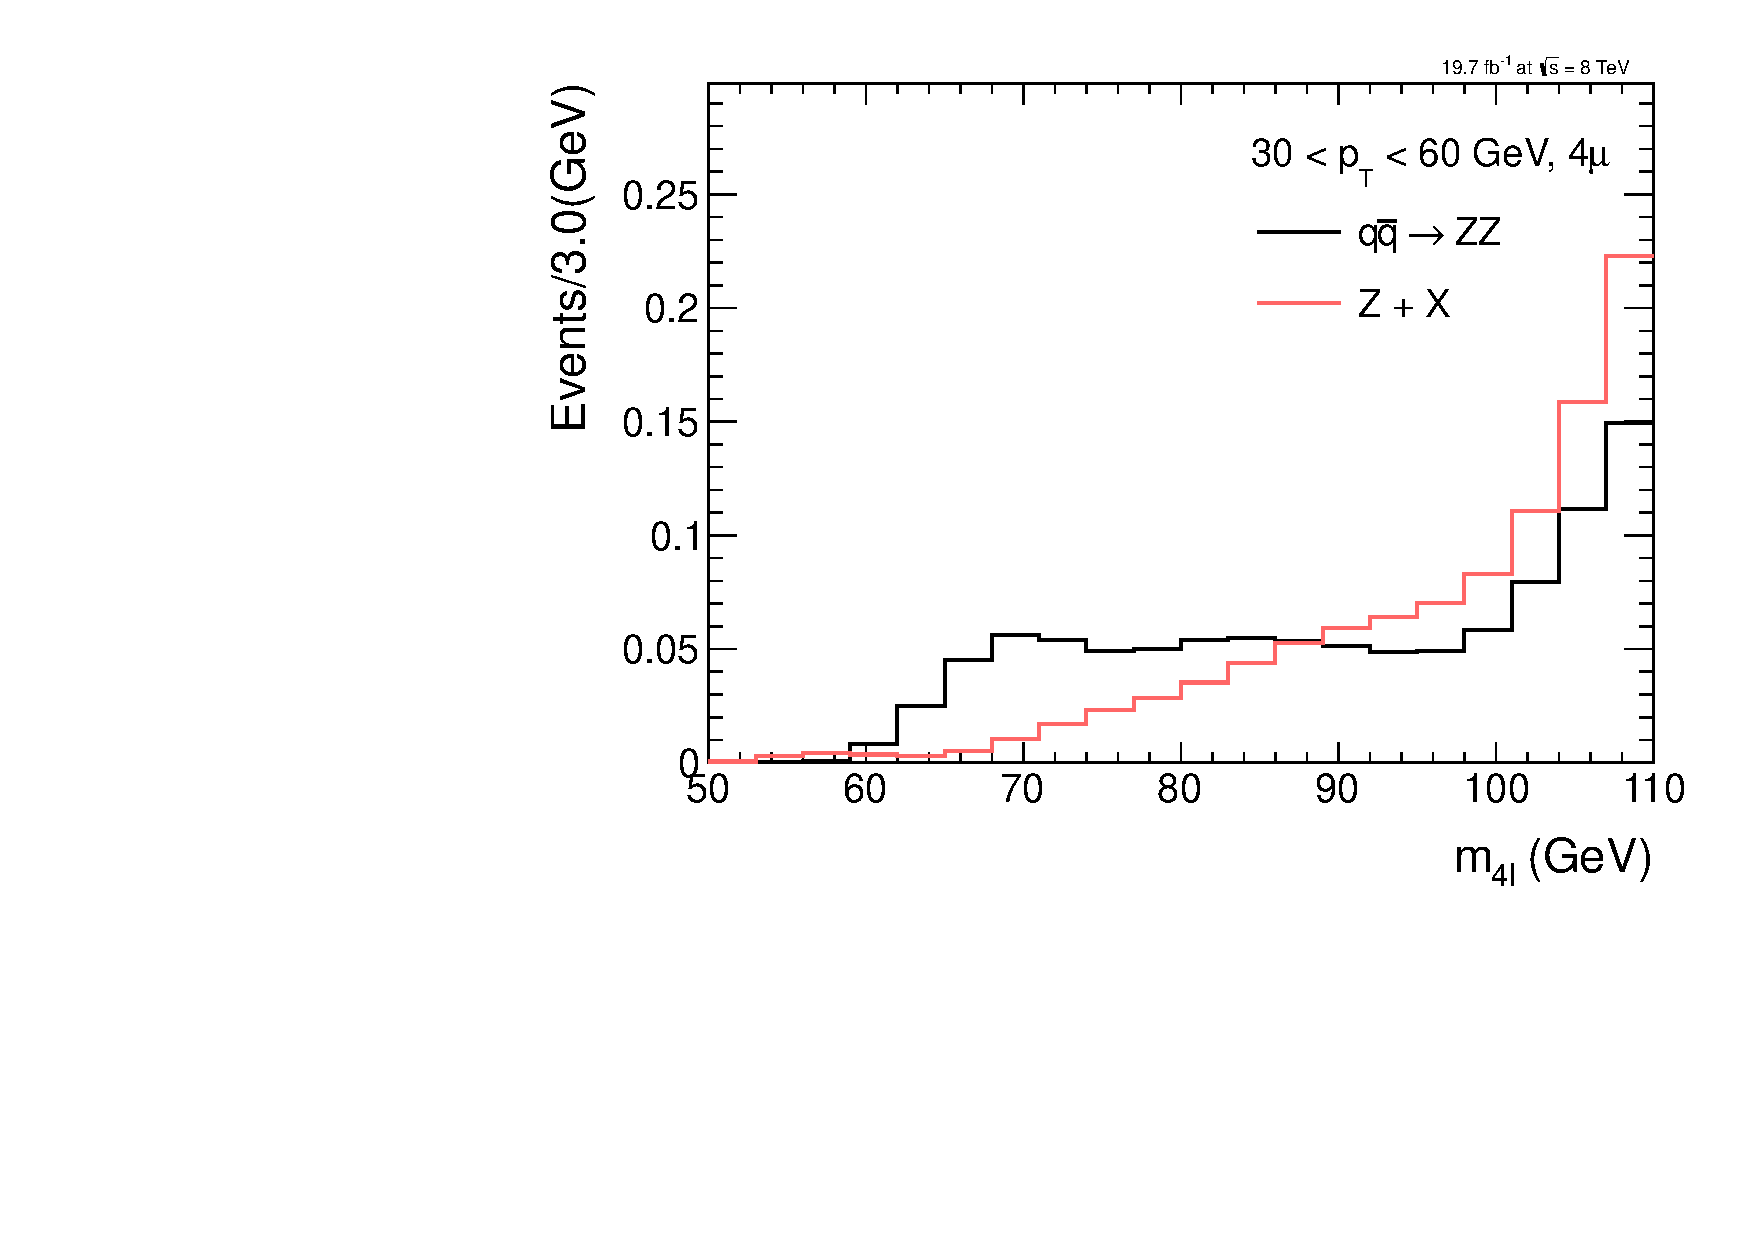
\includegraphics[width=0.32\textwidth,angle=0]{Appendix/figuresZ4l/XSTemplates_4mu_pT4l_30_60_qqZZ_ZJetsCR.pdf}
      \label{fig:z4l_bkg-pT4l-qqZZ-ZX-4mu:c}
    }
    \subfigure[$30.0 \GeV < \pt(4\ell) < 60.0 \GeV$]{
      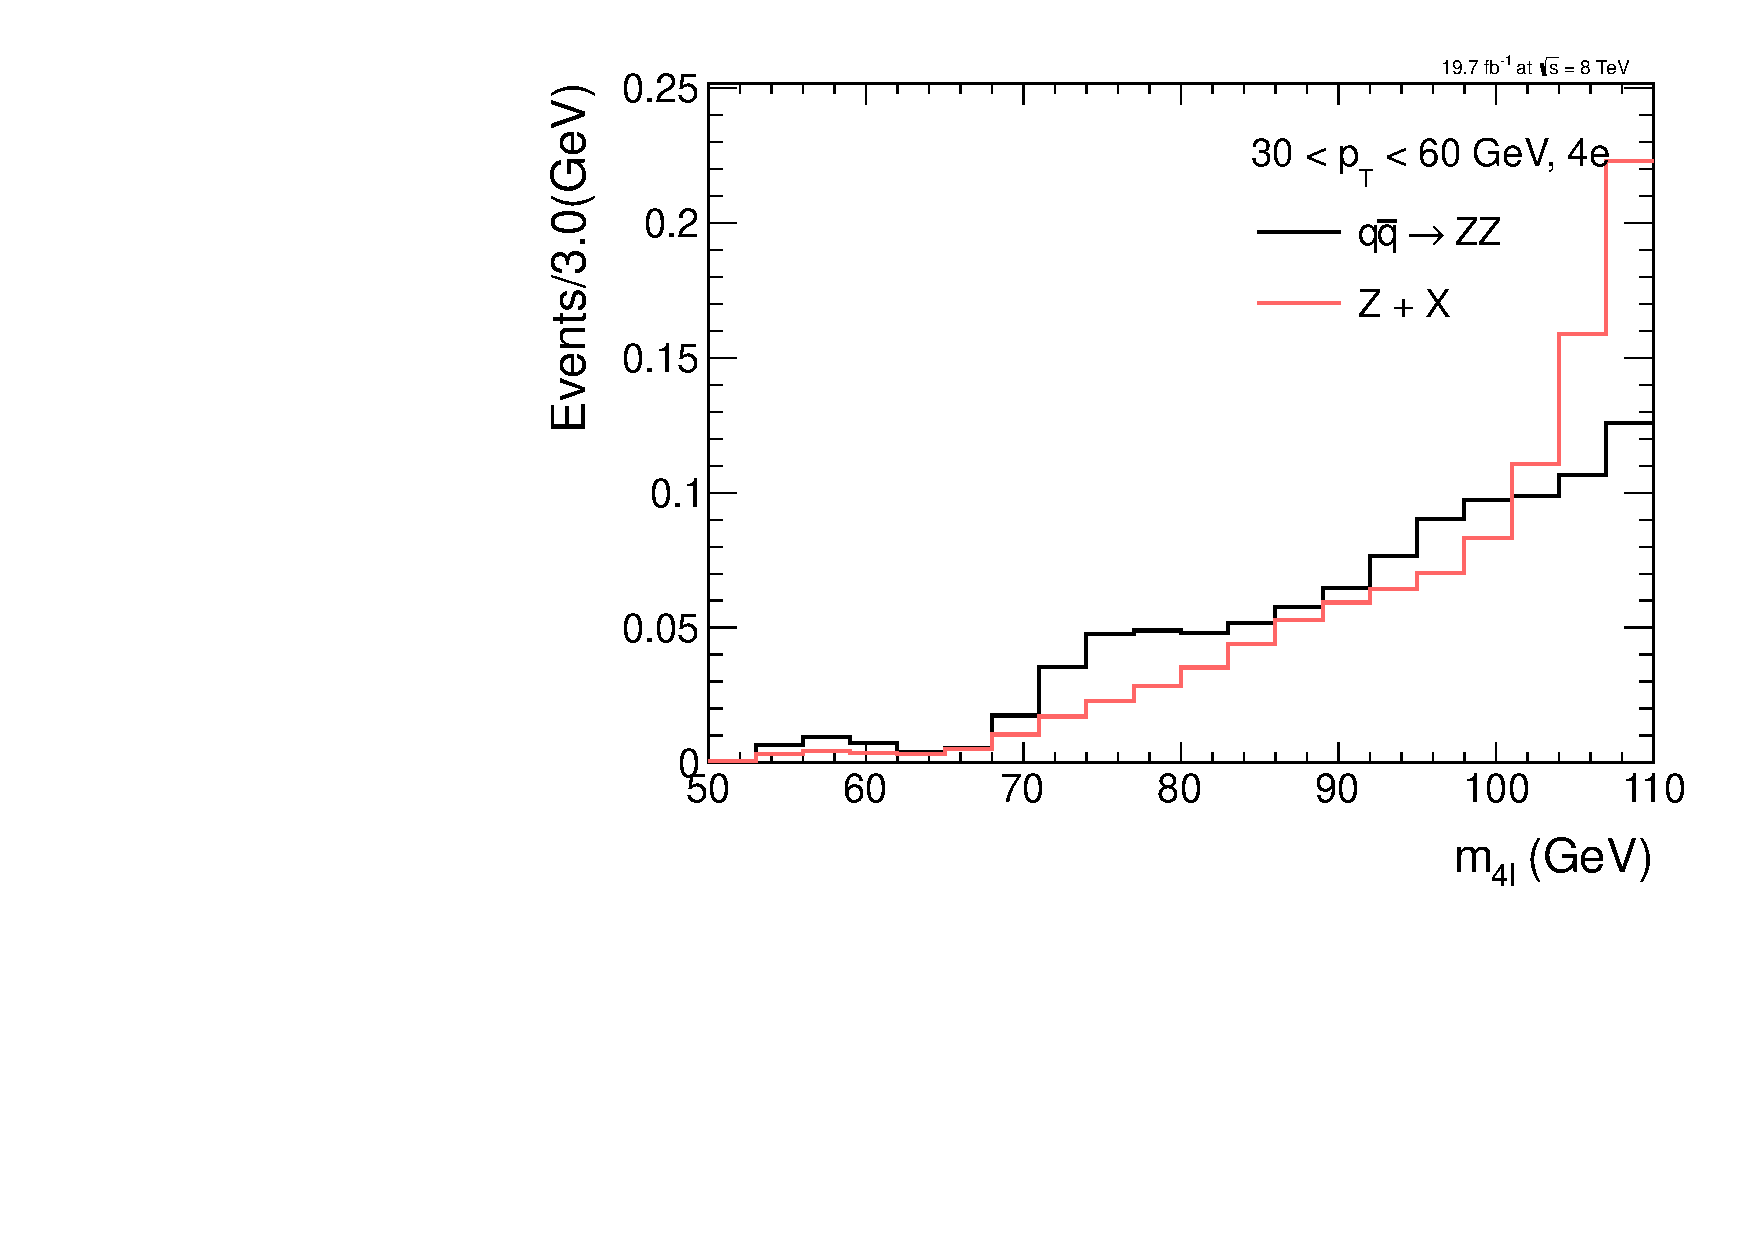
\includegraphics[width=0.32\textwidth,angle=0]{Appendix/figuresZ4l/XSTemplates_4e_pT4l_30_60_qqZZ_ZJetsCR.pdf}
      \label{fig:z4l_bkg-pT4l-qqZZ-ZX-4e:c}
    } \\
    
    \subfigure[$60.0 \GeV < \pt(4\ell) < 1000.0 \GeV$]{
      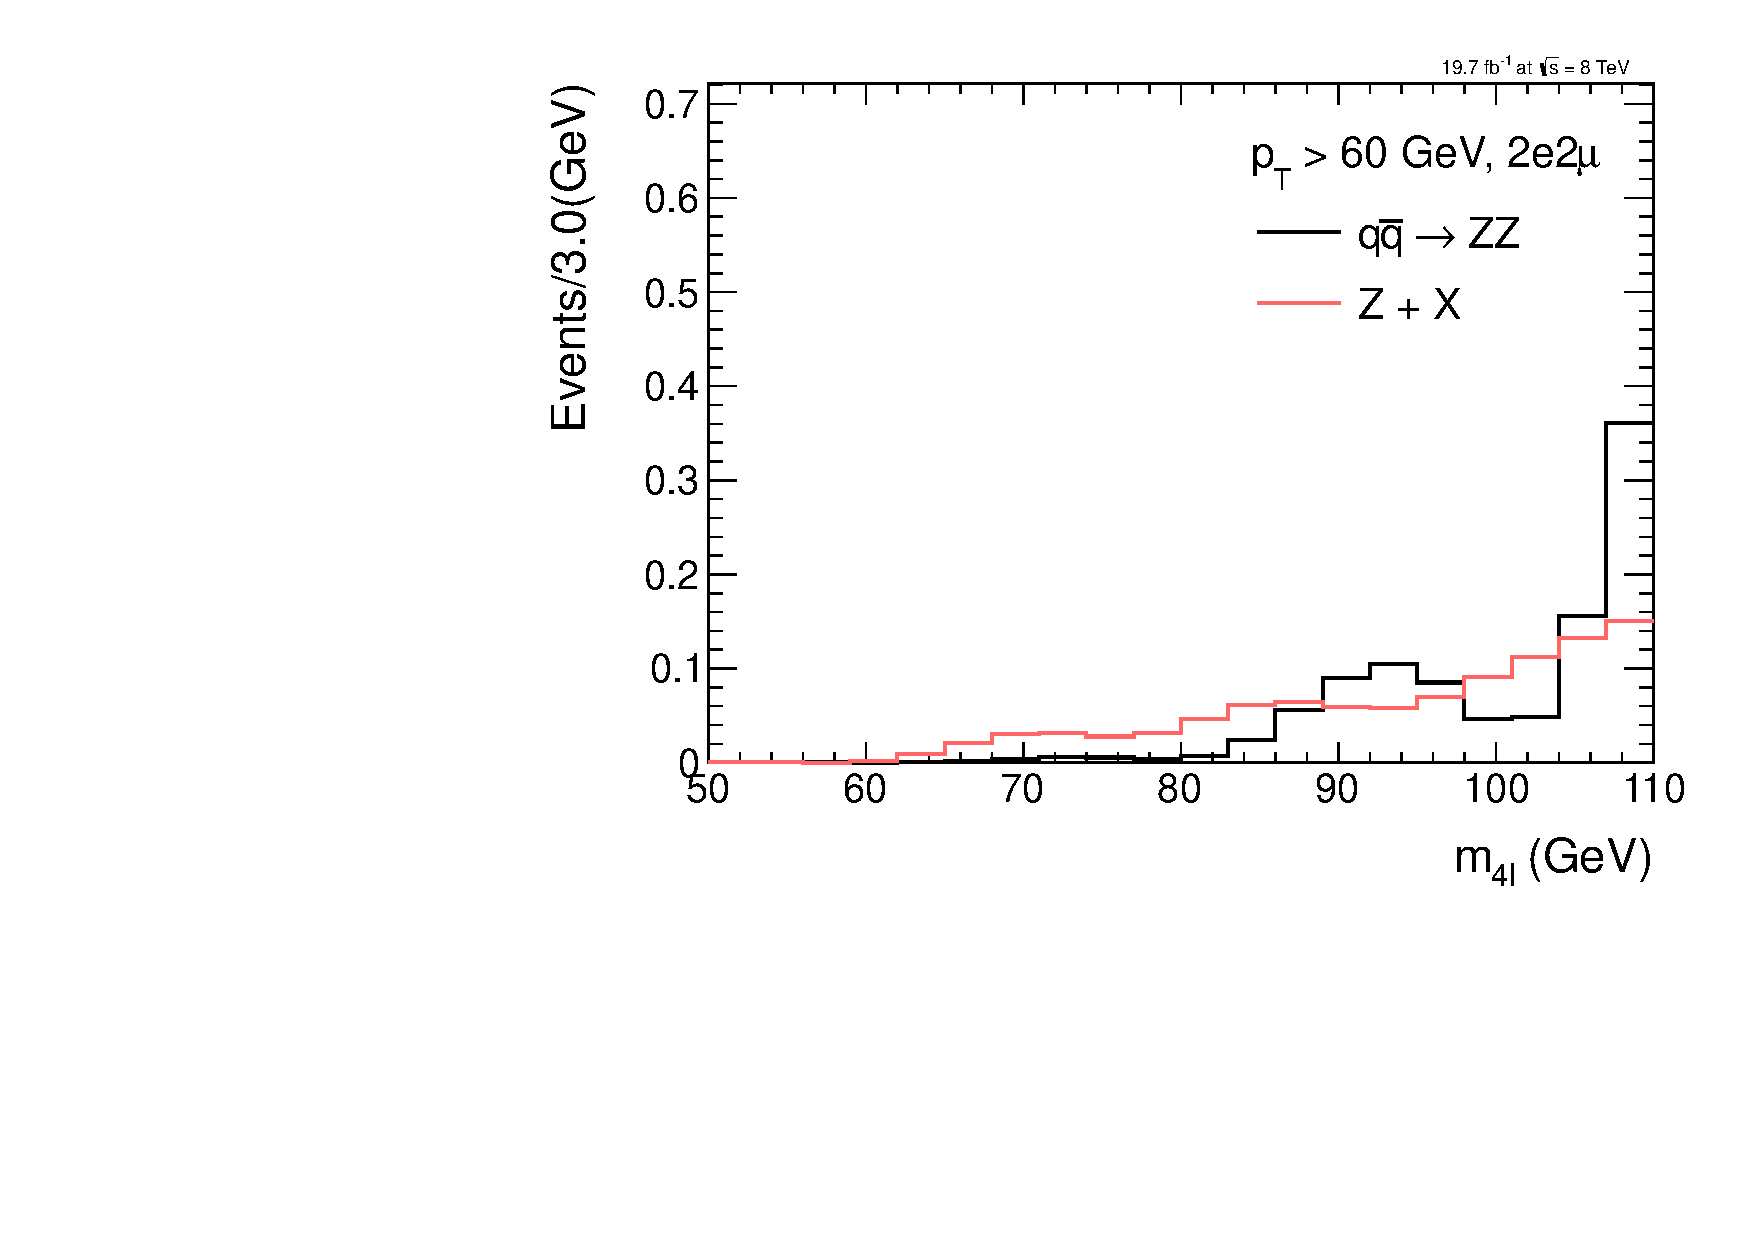
\includegraphics[width=0.32\textwidth,angle=0]{Appendix/figuresZ4l/XSTemplates_2e2mu_pT4l_60_1000_qqZZ_ZJetsCR.pdf}
      \label{fig:z4l_bkg-pT4l-qqZZ-ZX-2e2mu:d}
    }
    \subfigure[$60.0 \GeV < \pt(4\ell) < 1000.0 \GeV$]{
      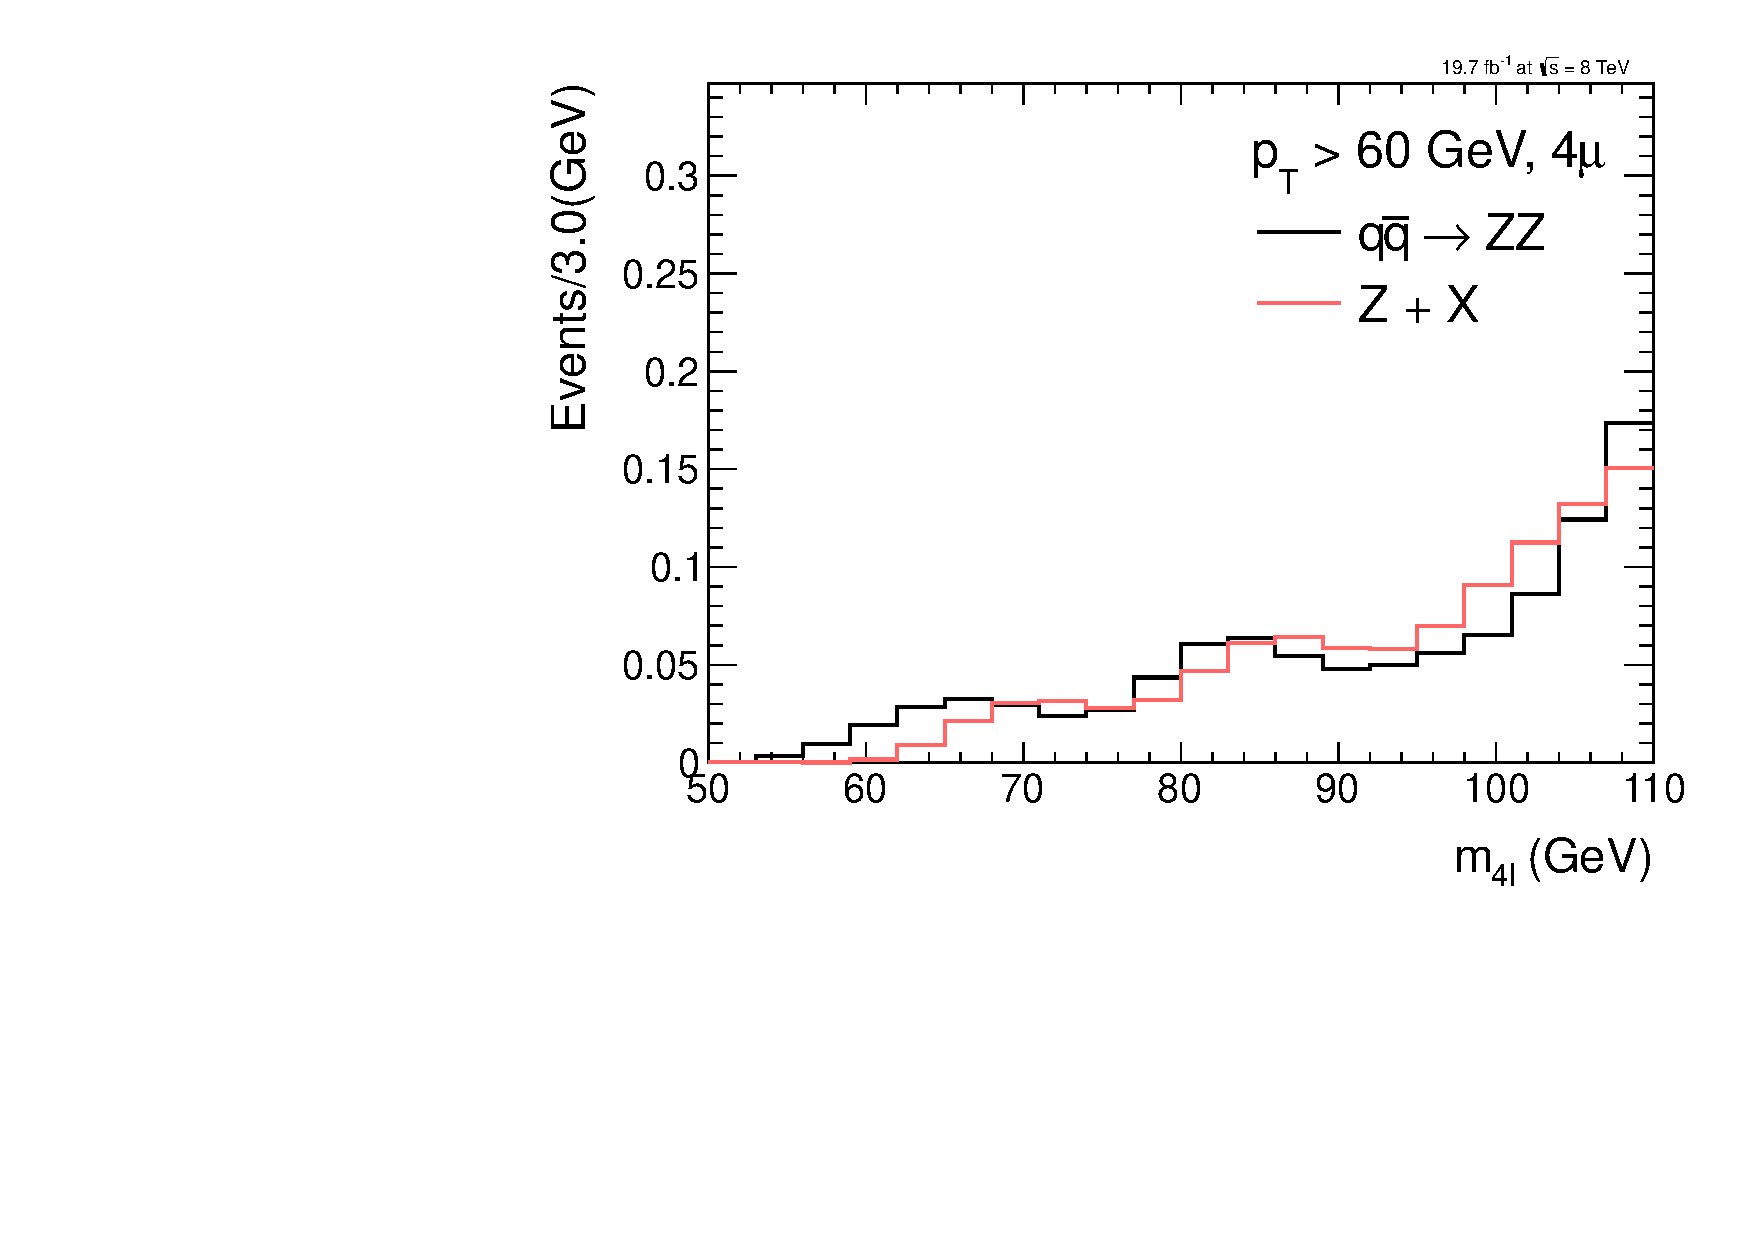
\includegraphics[width=0.32\textwidth,angle=0]{Appendix/figuresZ4l/XSTemplates_4mu_pT4l_60_1000_qqZZ_ZJetsCR.pdf}
      \label{fig:z4l_bkg-pT4l-qqZZ-ZX-4mu:d}
    }
    \subfigure[$60.0 \GeV < \pt(4\ell) < 1000.0 \GeV$]{
      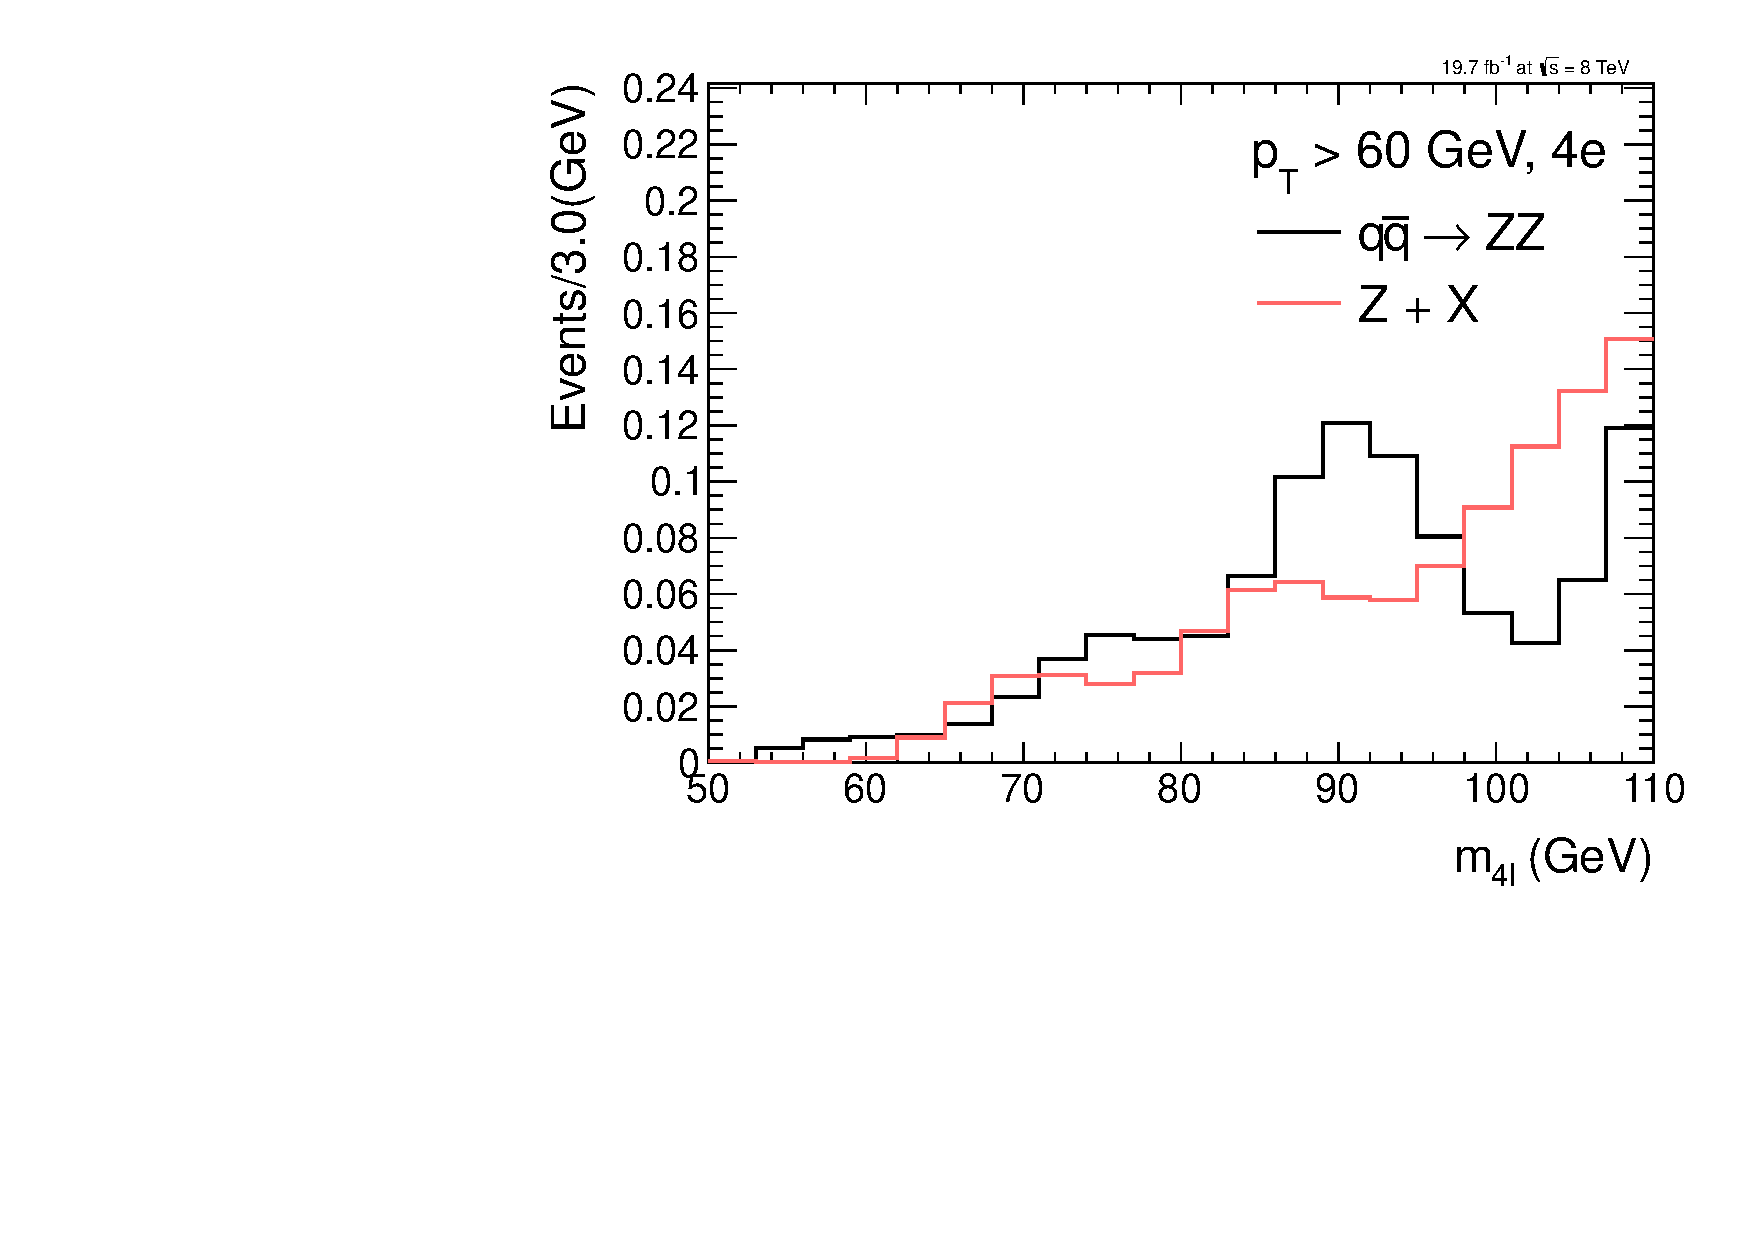
\includegraphics[width=0.32\textwidth,angle=0]{Appendix/figuresZ4l/XSTemplates_4e_pT4l_60_1000_qqZZ_ZJetsCR.pdf}
      \label{fig:z4l_bkg-pT4l-qqZZ-ZX-4e:d}
    } \\
    
    \caption{ Distributions of m($4\ell$) for the $qq \rightarrow \mathrm{ZZ}$ and Z+X backgrounds in different bins of $\pt(4\ell)$ 
for Z$\to$4l measurements
    for three final states: $2e2\mu$(left), $4\mu$(middle) and $4e$(right).}
  \label{fig:z4l_bkg-pT4l-qqZZ-ZX}
  
 \end{center}
\end{figure} 

 \clearpage
 
 \begin{figure}[!ht]
  \begin{center}
  
    \subfigure[$0.0 \GeV < \pt(4\ell) < 15.0 \GeV$]{
      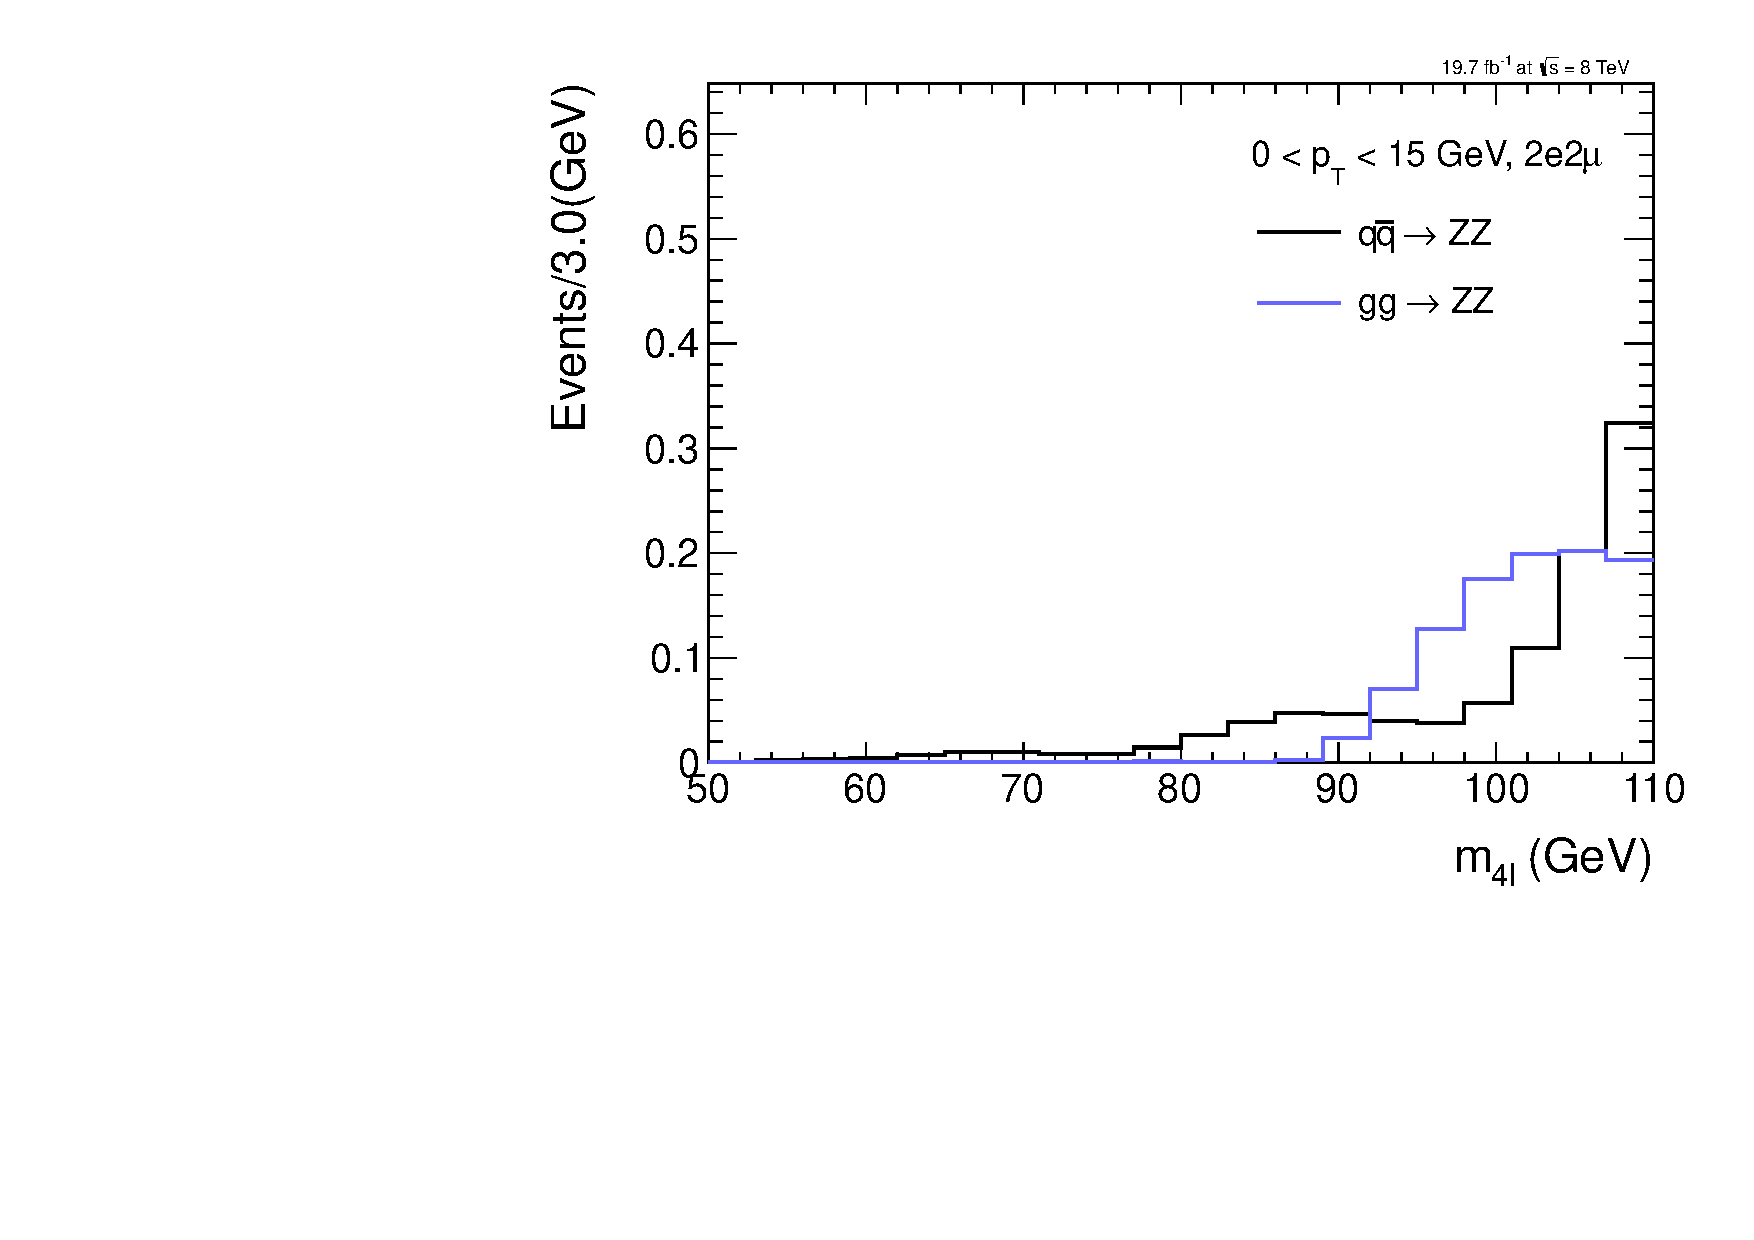
\includegraphics[width=0.32\textwidth,angle=0]{Appendix/figuresZ4l/XSTemplates_2e2mu_pT4l_0_15_qqZZ_ggZZ.pdf}
      \label{fig:z4l_bkg-pT4l-qqZZ-ggZZ-2e2mu:a}
    }    
    \subfigure[$0.0 \GeV < \pt(4\ell) < 15.0 \GeV$]{
      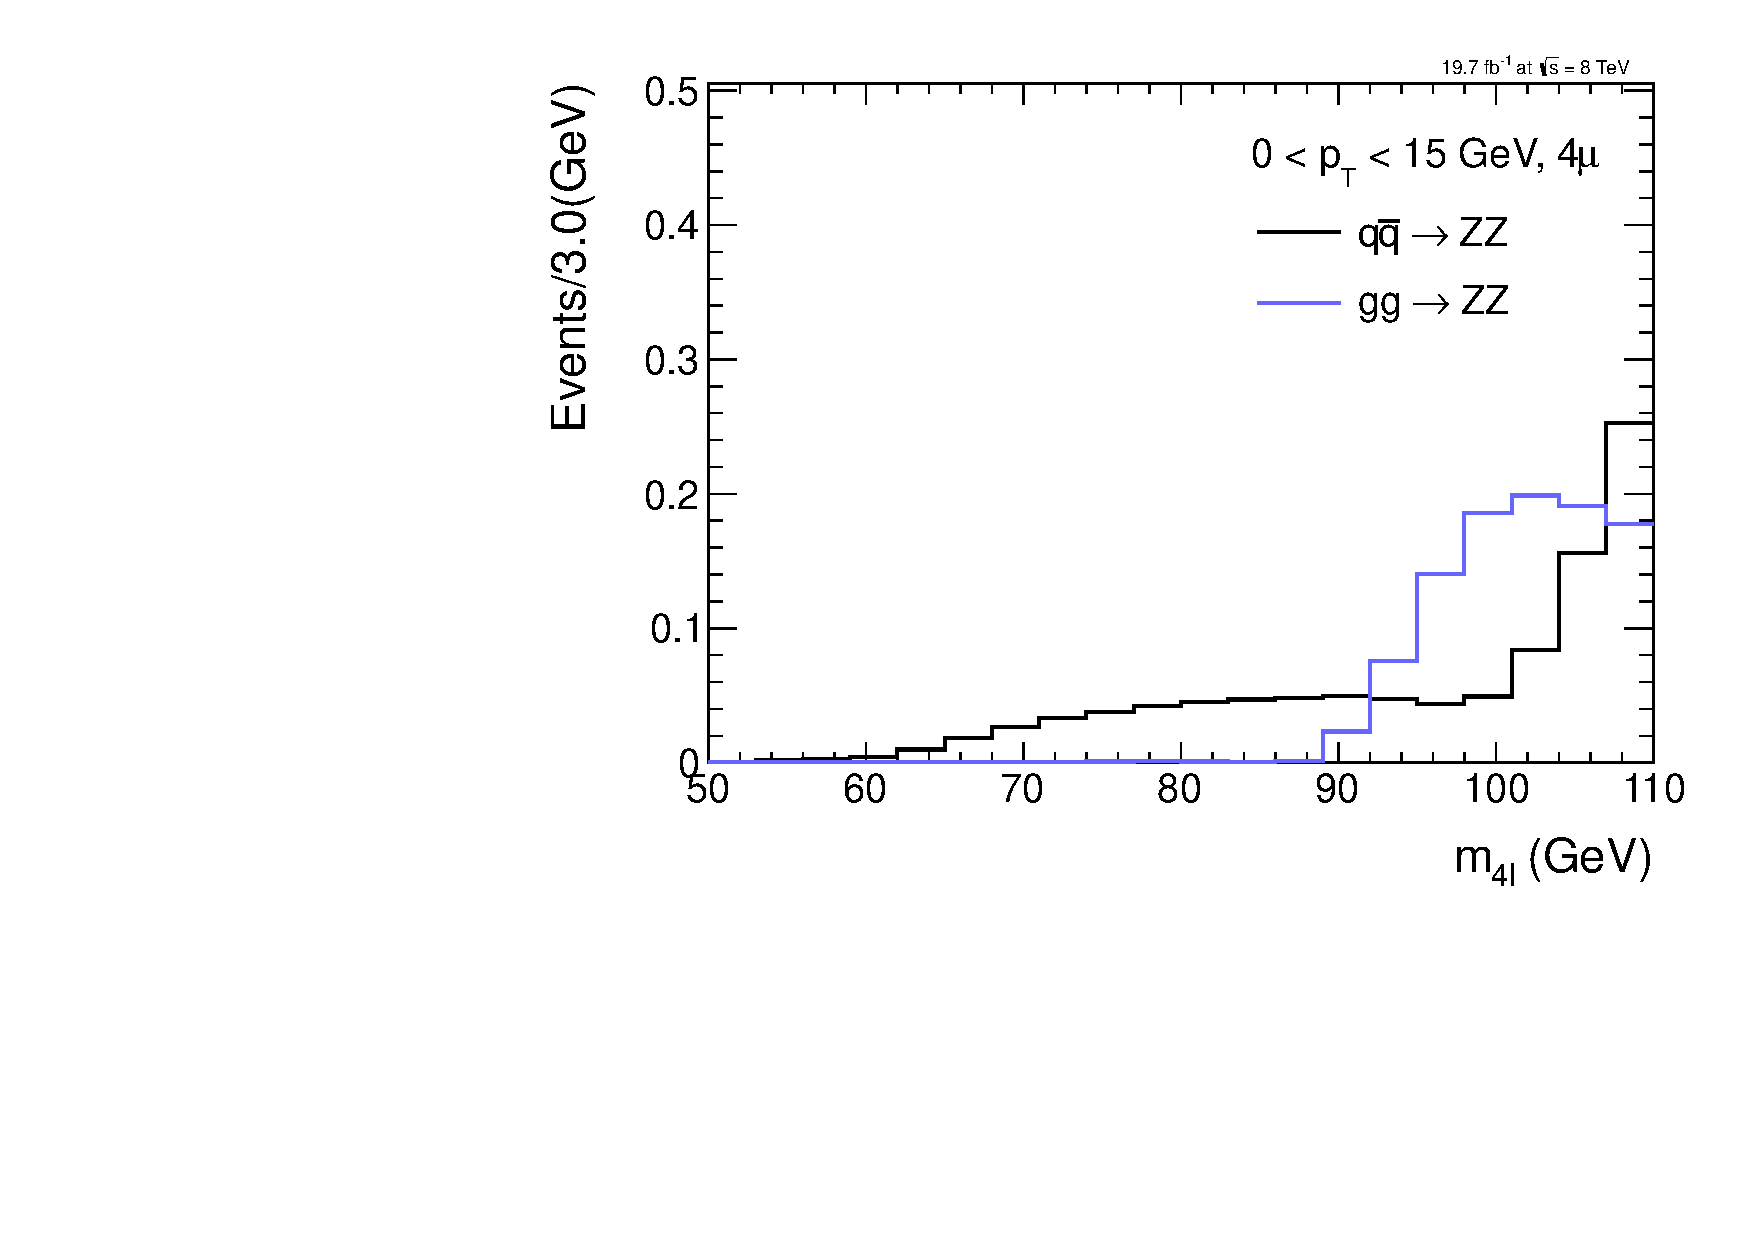
\includegraphics[width=0.32\textwidth,angle=0]{Appendix/figuresZ4l/XSTemplates_4mu_pT4l_0_15_qqZZ_ggZZ.pdf}
      \label{fig:z4l_bkg-pT4l-qqZZ-ggZZ-4mu:a}
    }    
    \subfigure[$0.0 \GeV < \pt(4\ell) < 15.0 \GeV$]{
      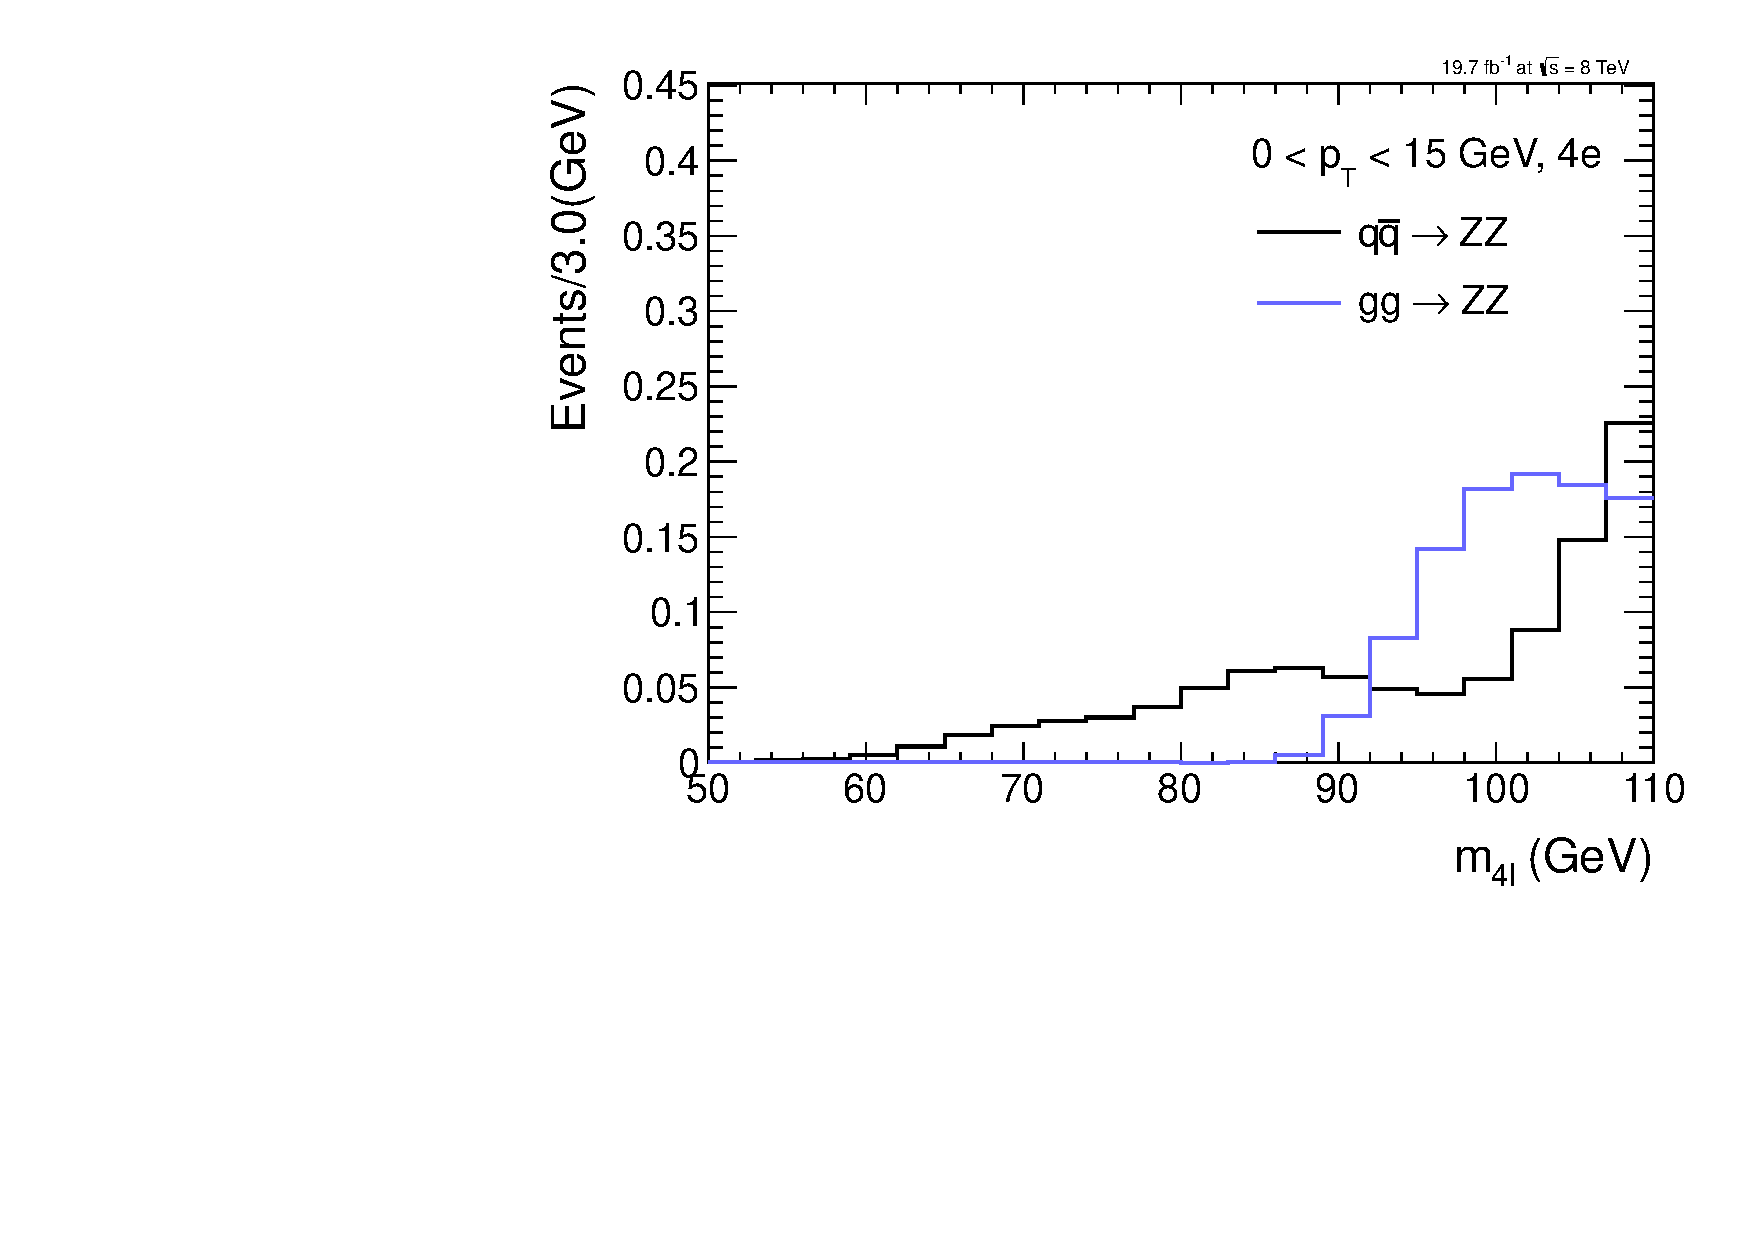
\includegraphics[width=0.32\textwidth,angle=0]{Appendix/figuresZ4l/XSTemplates_4e_pT4l_0_15_qqZZ_ggZZ.pdf}
      \label{fig:z4l_bkg-pT4l-qqZZ-ggZZ-4e:a}
    }    \\

    \subfigure[$15.0 \GeV < \pt(4\ell) < 30.0 \GeV$]{
      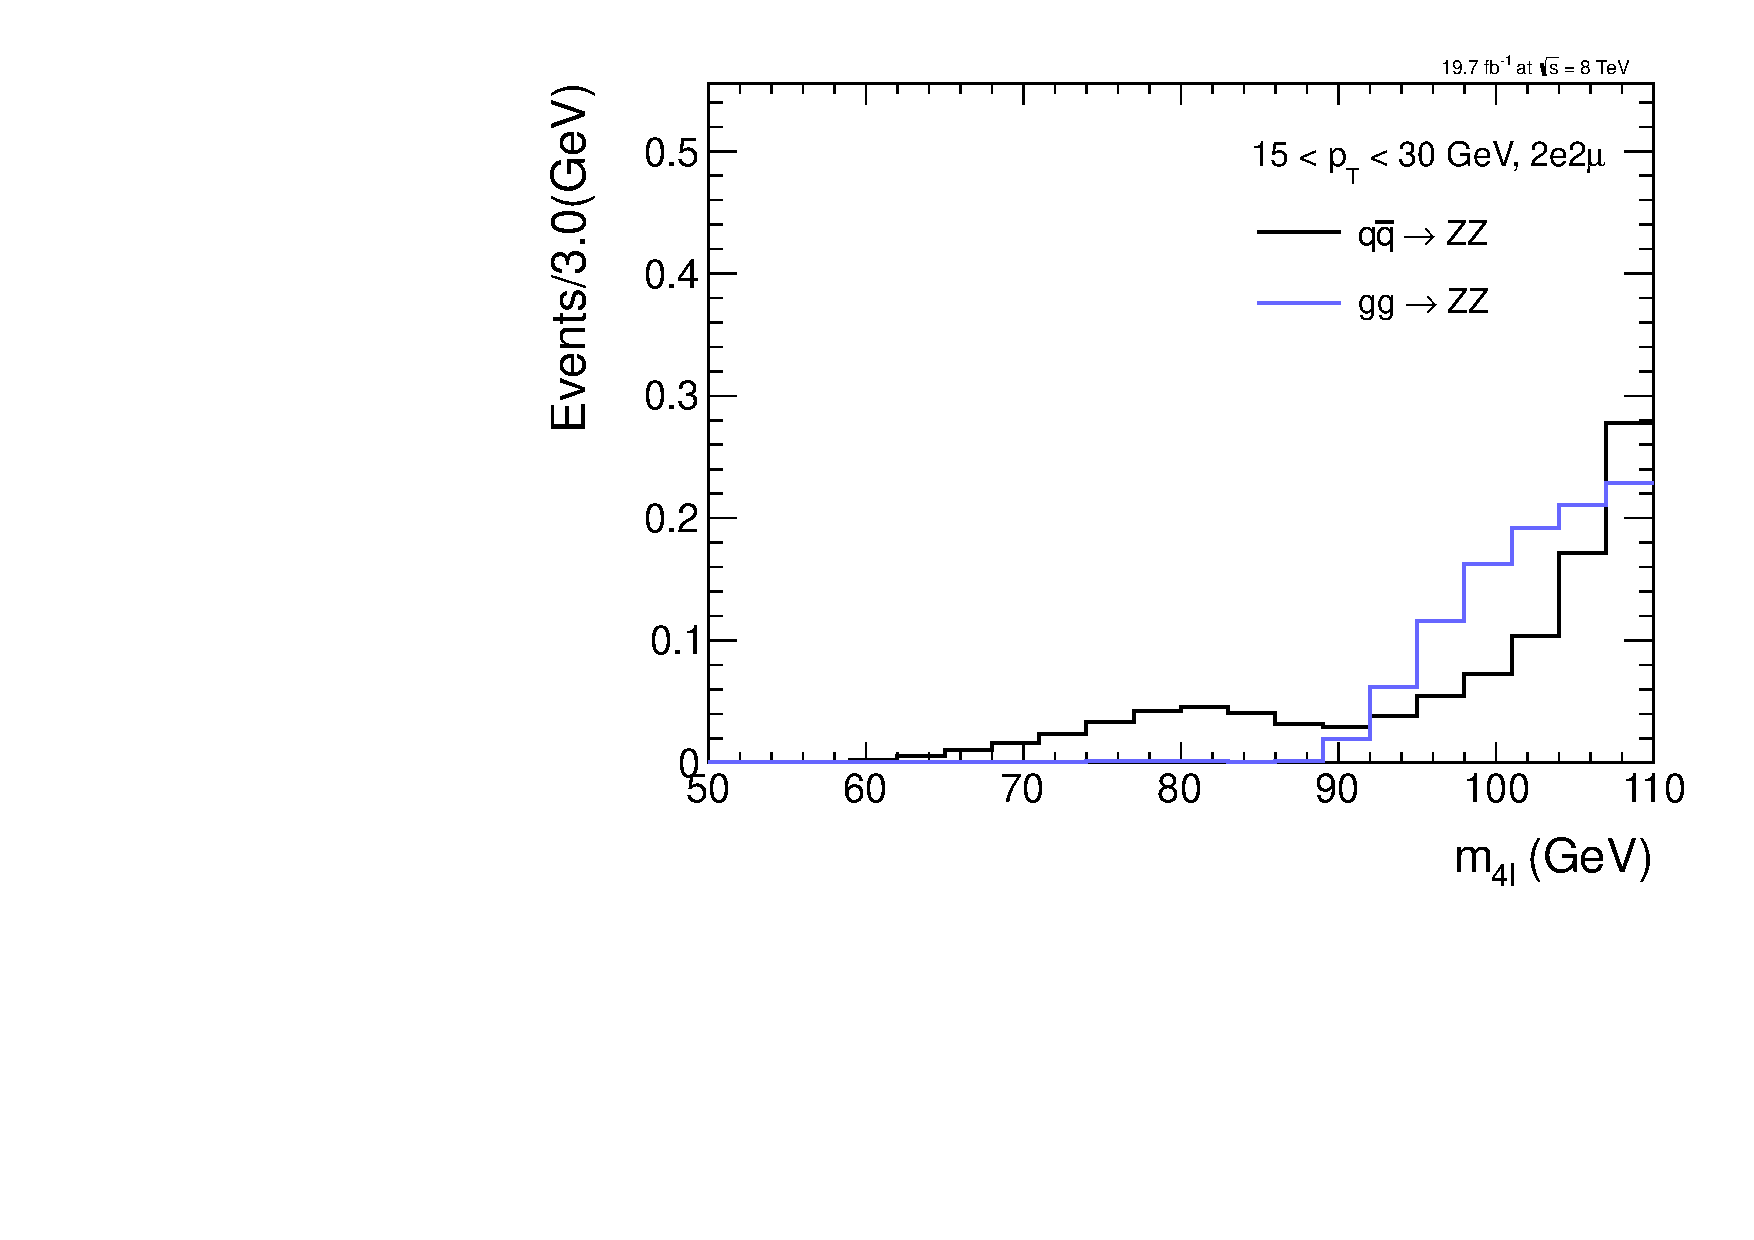
\includegraphics[width=0.32\textwidth,angle=0]{Appendix/figuresZ4l/XSTemplates_2e2mu_pT4l_15_30_qqZZ_ggZZ.pdf}
      \label{fig:z4l_bkg-pT4l-qqZZ-ggZZ-2e2mu:b}
    }
    \subfigure[$15.0 \GeV < \pt(4\ell) < 30.0 \GeV$]{
      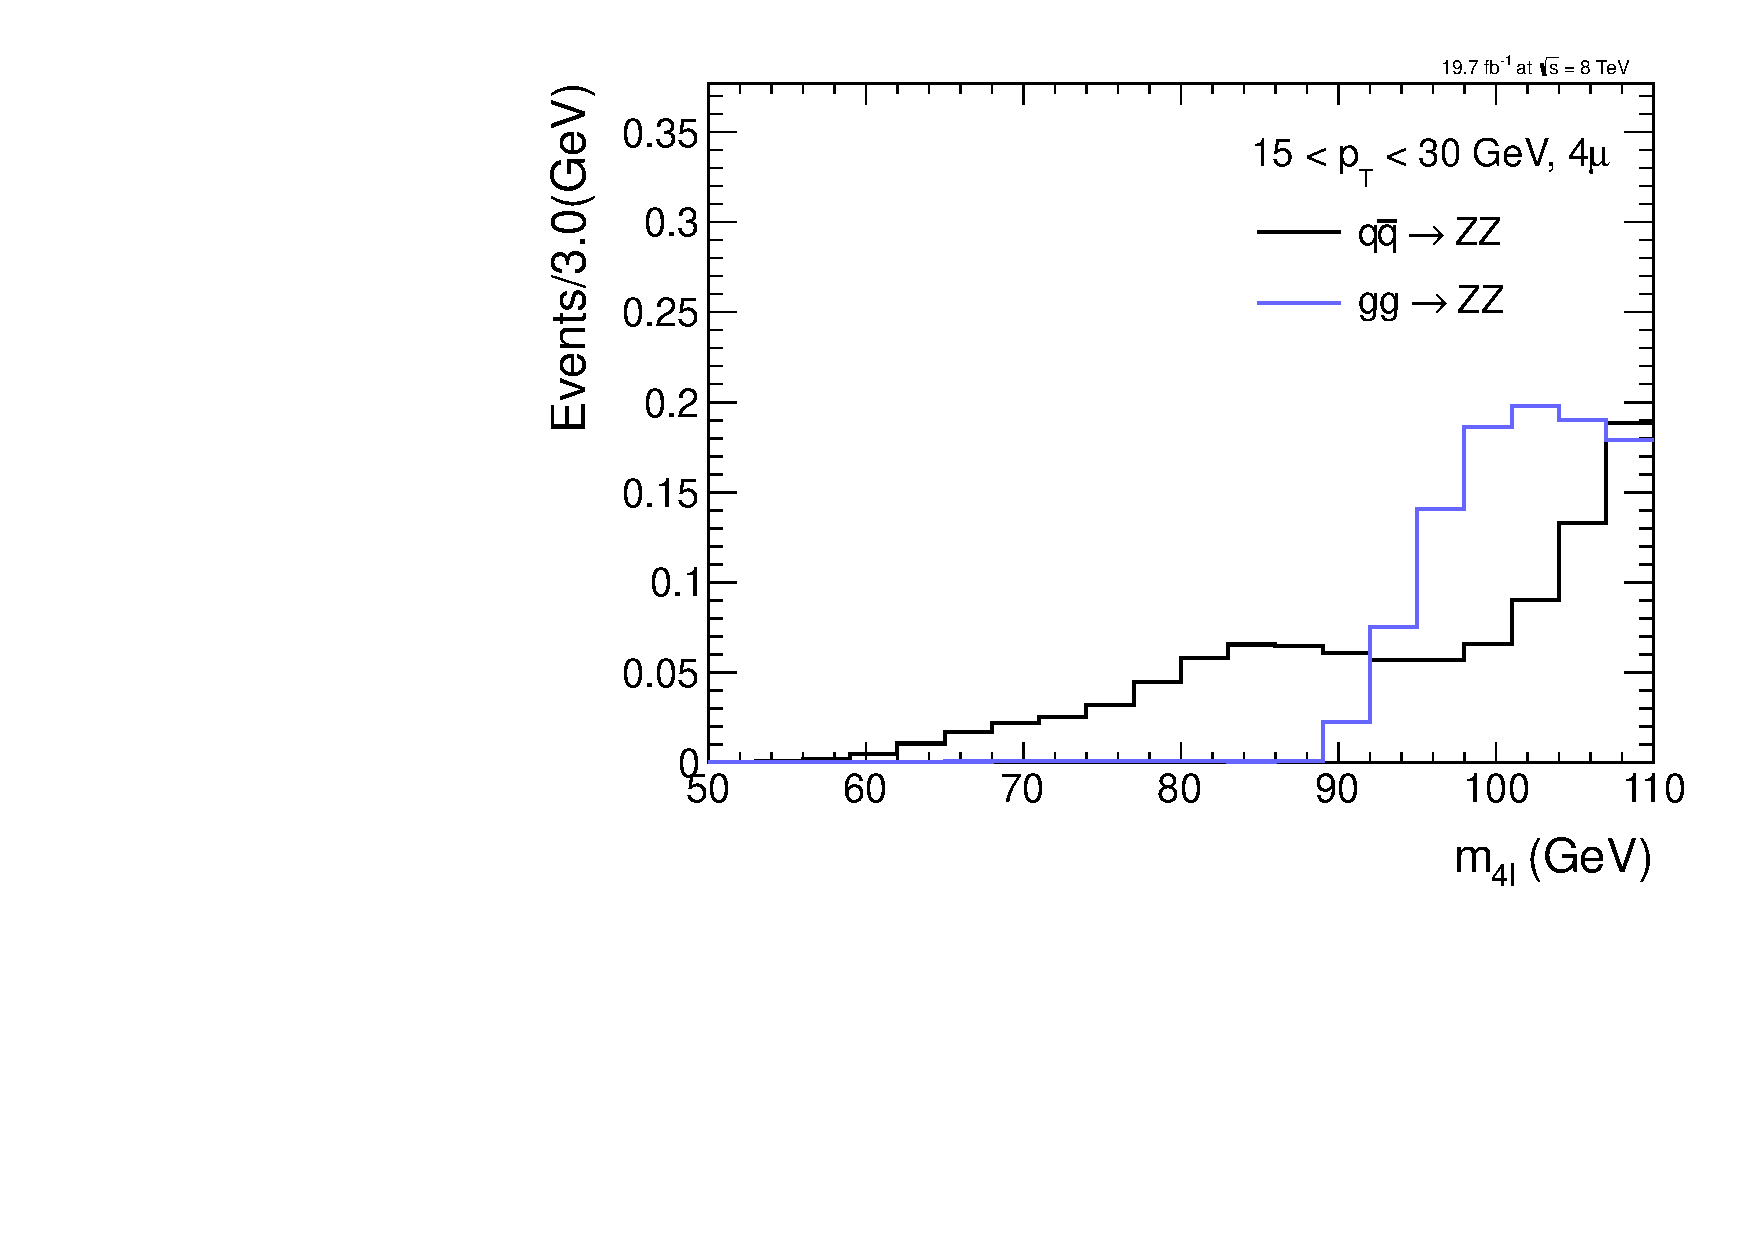
\includegraphics[width=0.32\textwidth,angle=0]{Appendix/figuresZ4l/XSTemplates_4mu_pT4l_15_30_qqZZ_ggZZ.pdf}
      \label{fig:z4l_bkg-pT4l-qqZZ-ggZZ-4mu:b}
    } 
    \subfigure[$15.0 \GeV < \pt(4\ell) < 30.0 \GeV$]{
      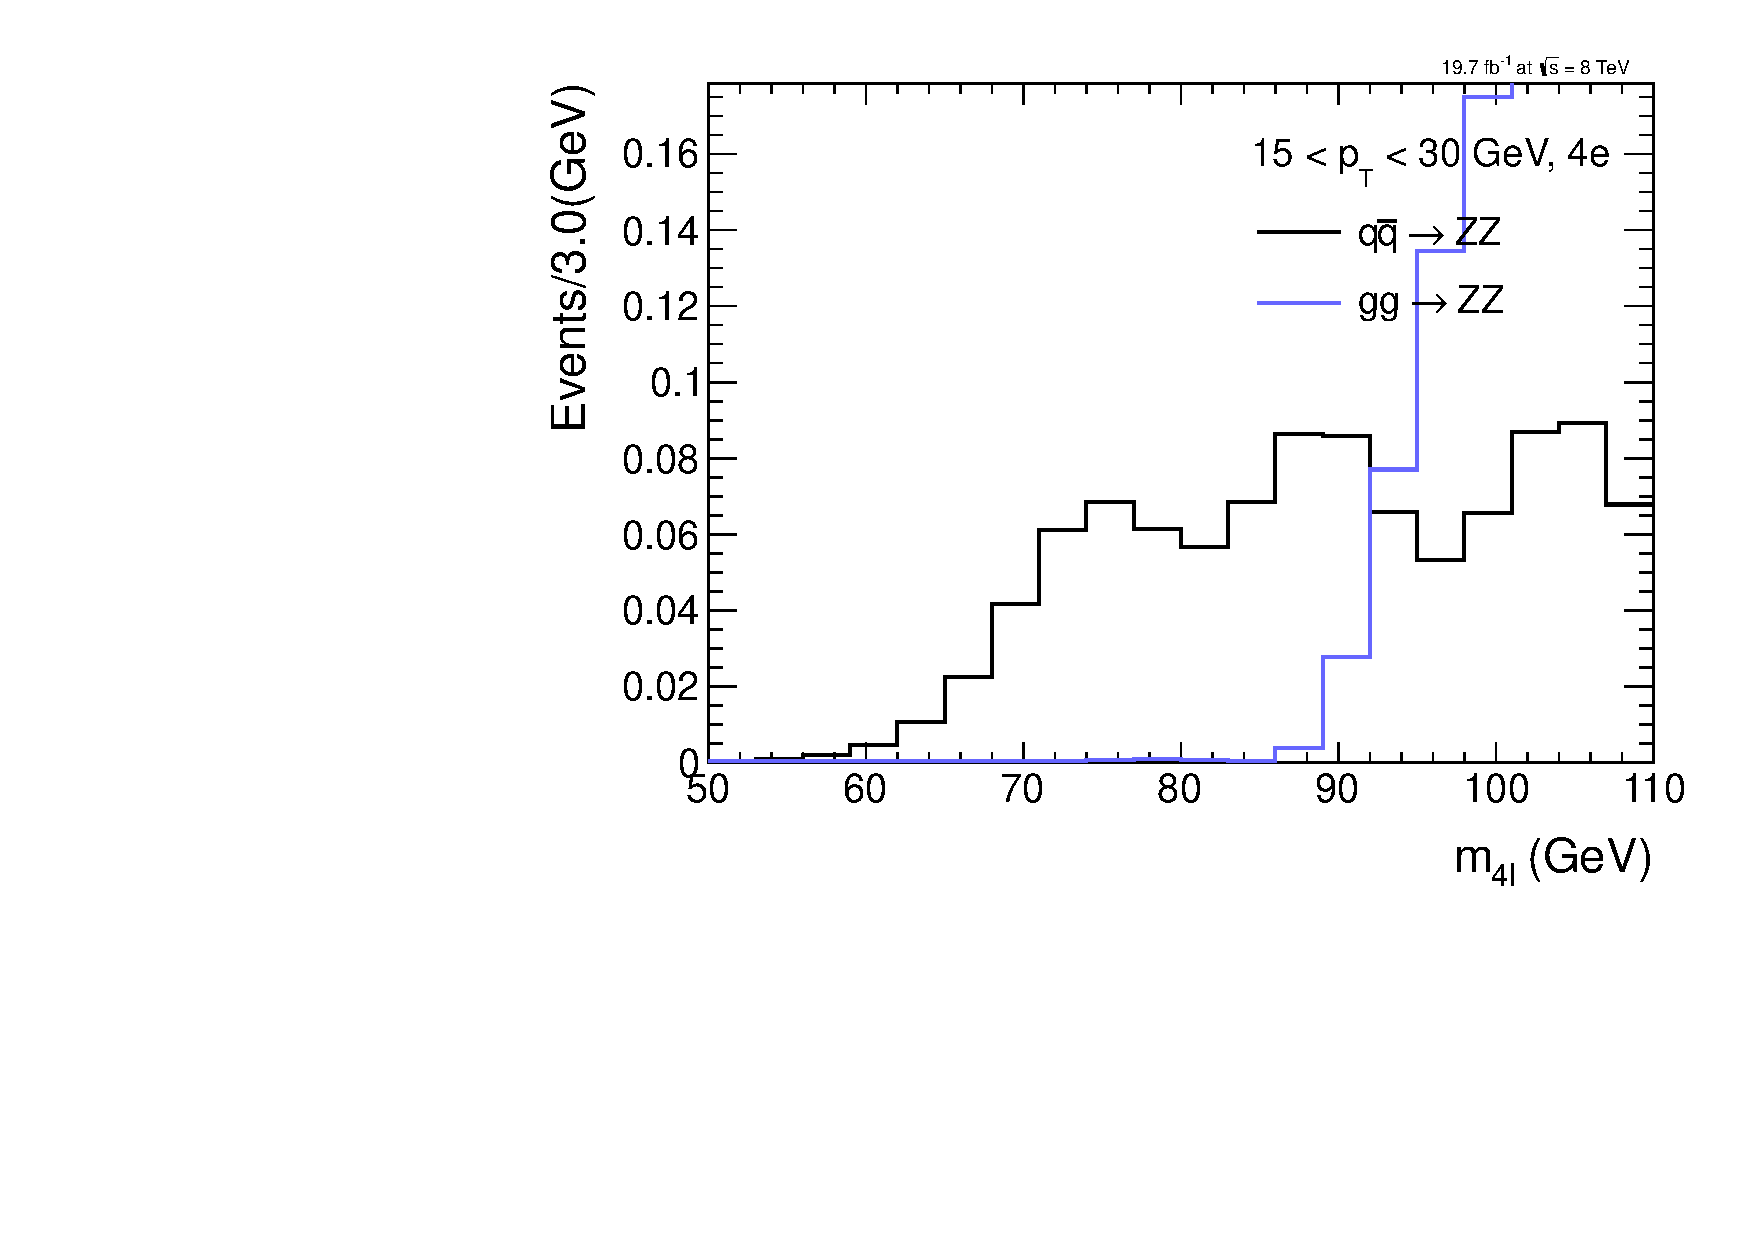
\includegraphics[width=0.32\textwidth,angle=0]{Appendix/figuresZ4l/XSTemplates_4e_pT4l_15_30_qqZZ_ggZZ.pdf}
      \label{fig:z4l_bkg-pT4l-qqZZ-ggZZ-4e:b}
    } \\
    
    \subfigure[$30.0 \GeV < \pt(4\ell) < 60.0 \GeV$]{
      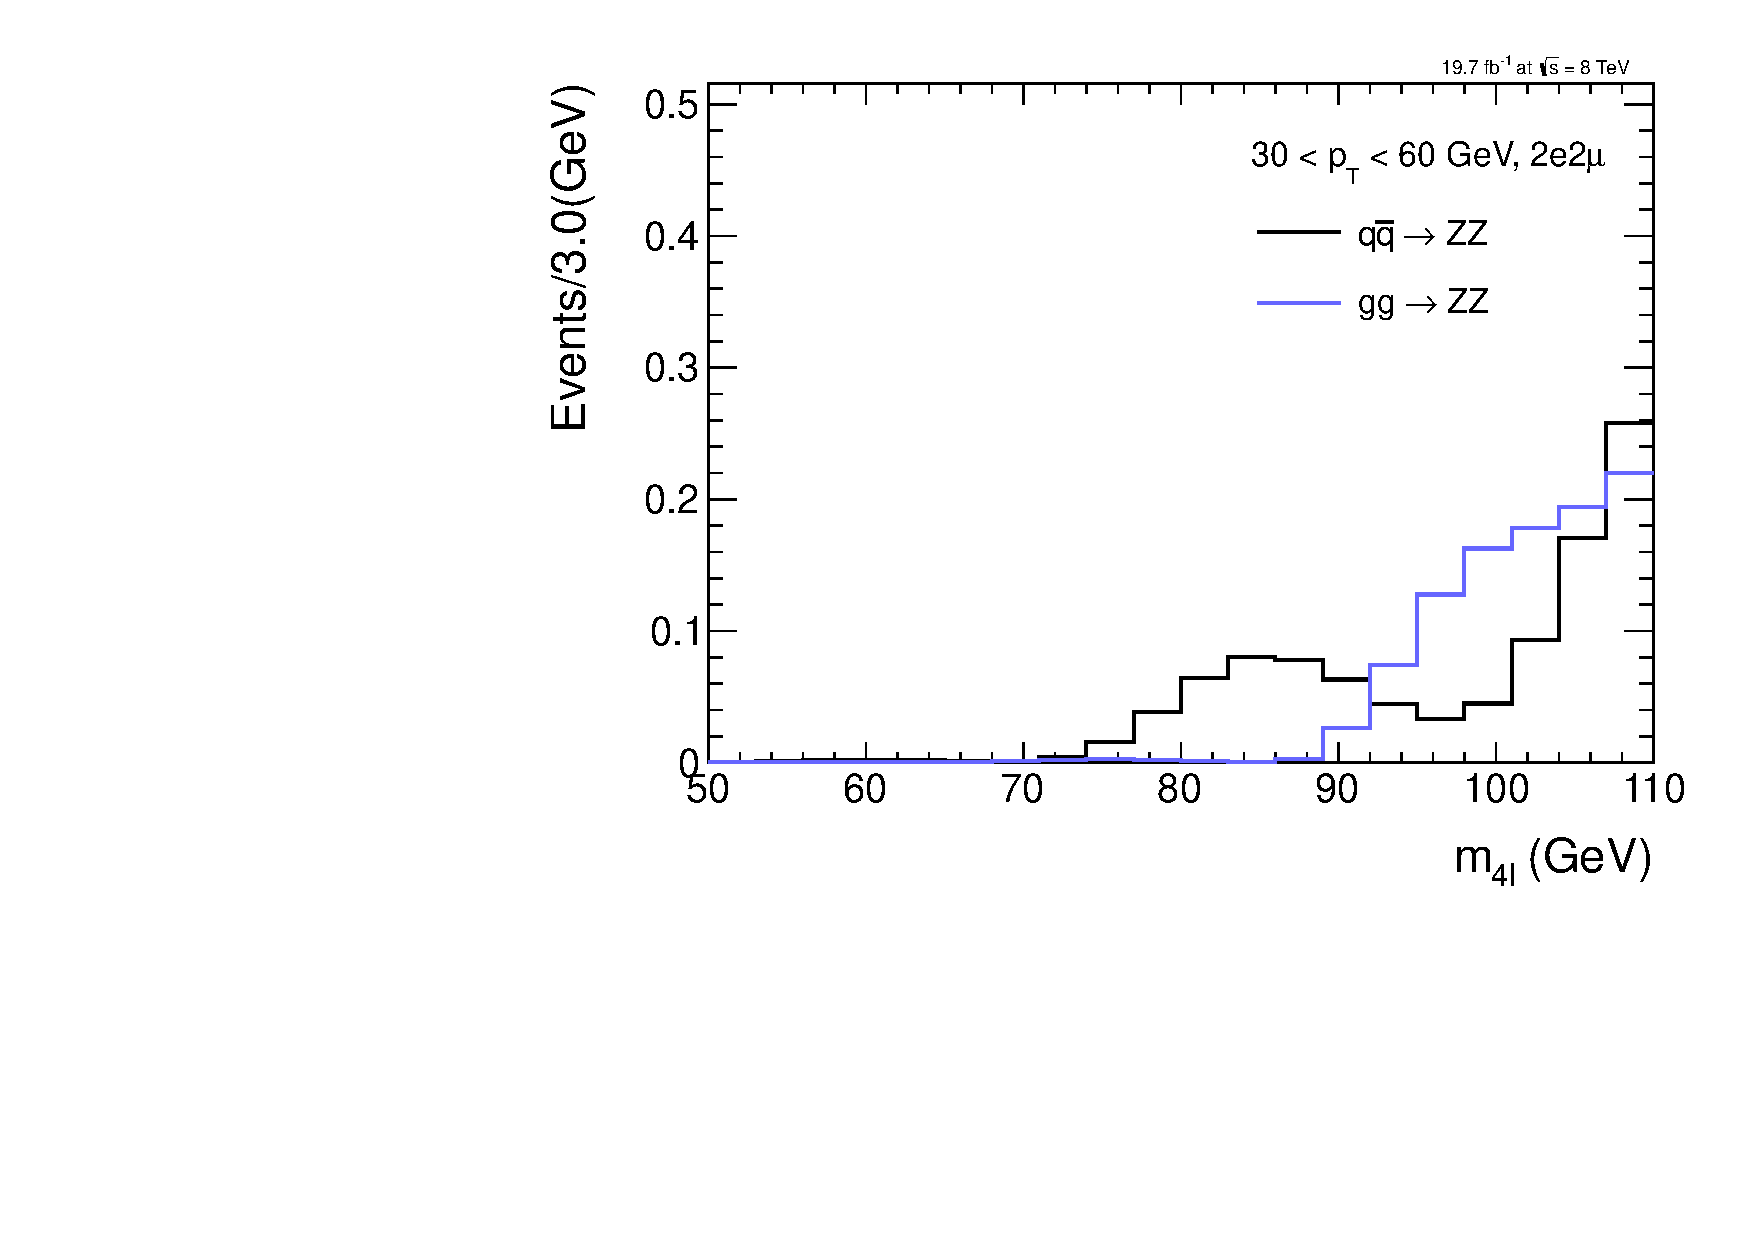
\includegraphics[width=0.32\textwidth,angle=0]{Appendix/figuresZ4l/XSTemplates_2e2mu_pT4l_30_60_qqZZ_ggZZ.pdf}
      \label{fig:z4l_bkg-pT4l-qqZZ-ggZZ-2e2mu:c}
    }
    \subfigure[$30.0 \GeV < \pt(4\ell) < 60.0 \GeV$]{
      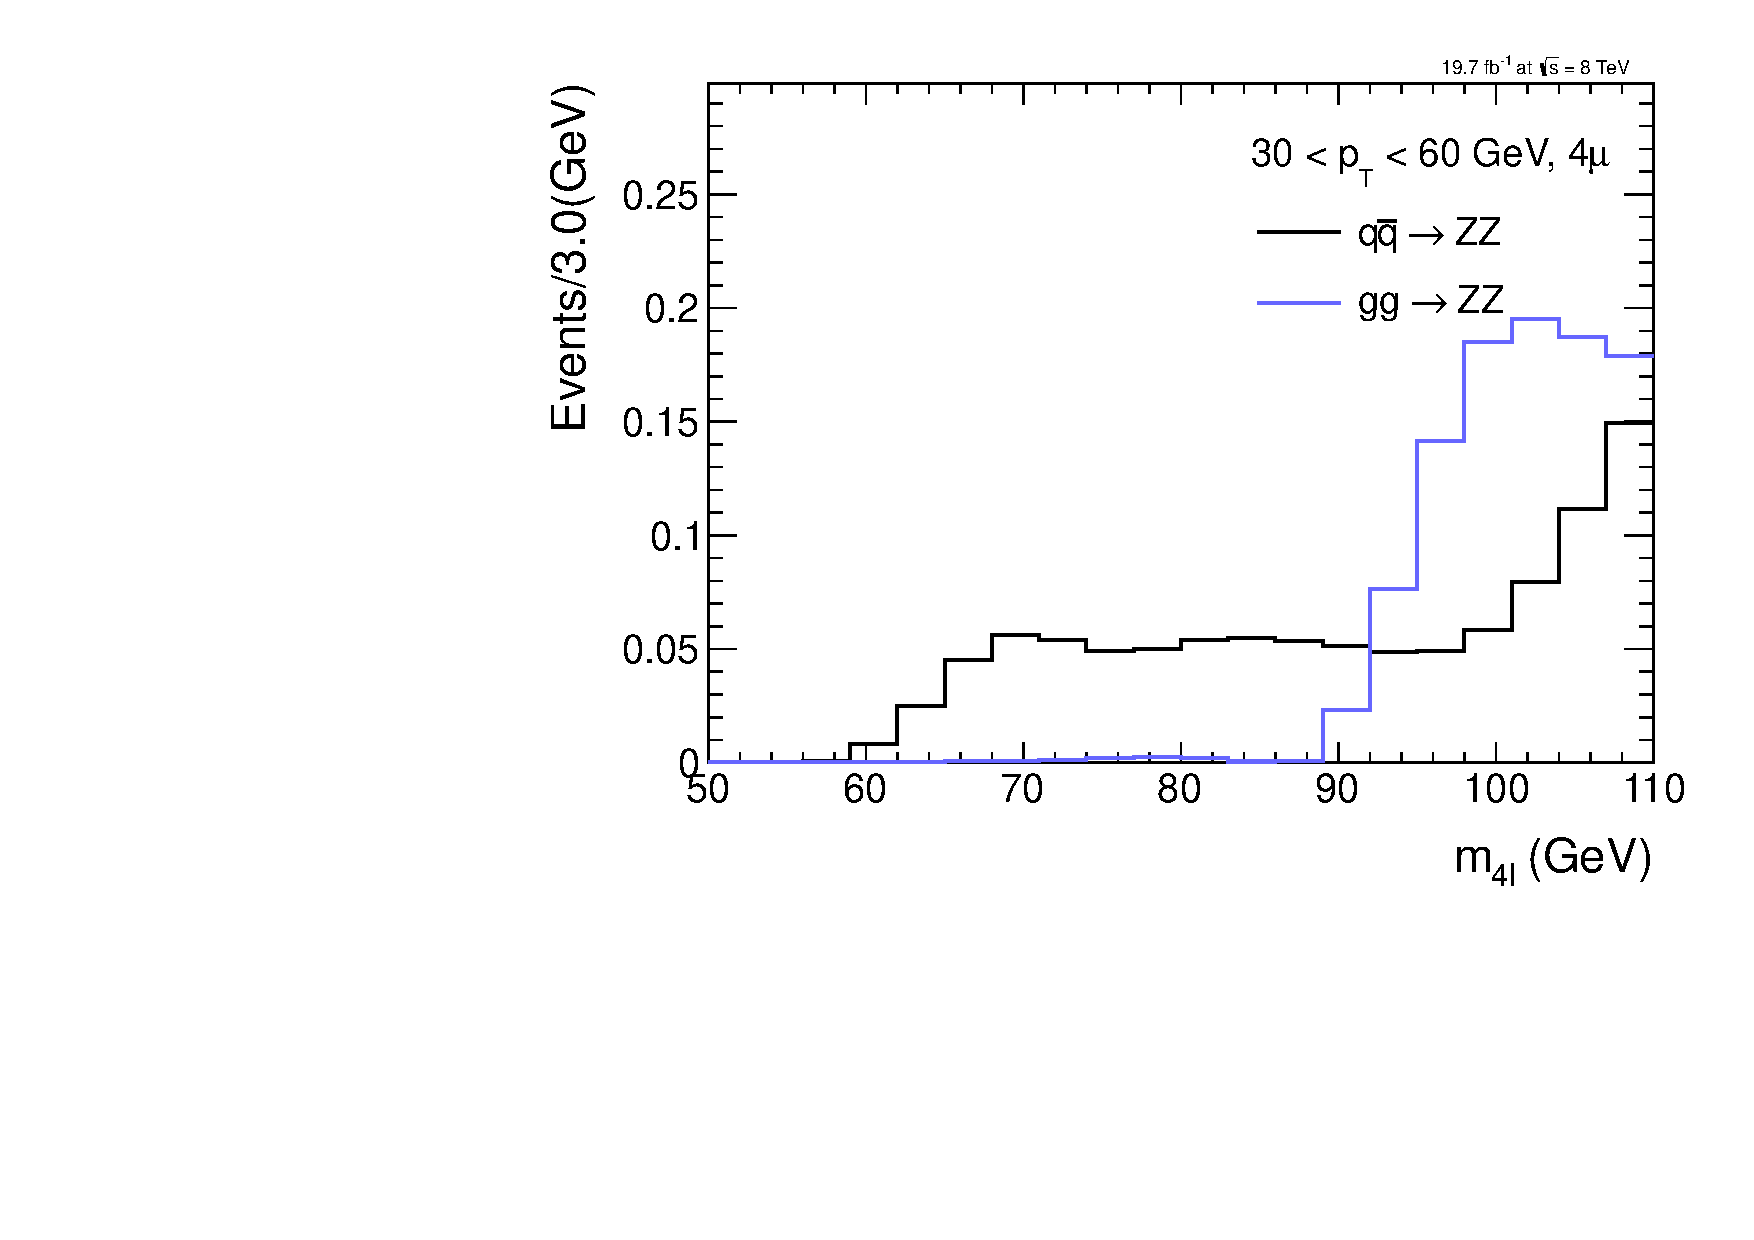
\includegraphics[width=0.32\textwidth,angle=0]{Appendix/figuresZ4l/XSTemplates_4mu_pT4l_30_60_qqZZ_ggZZ.pdf}
      \label{fig:z4l_bkg-pT4l-qqZZ-ggZZ-4mu:c}
    }
    \subfigure[$30.0 \GeV < \pt(4\ell) < 60.0 \GeV$]{
      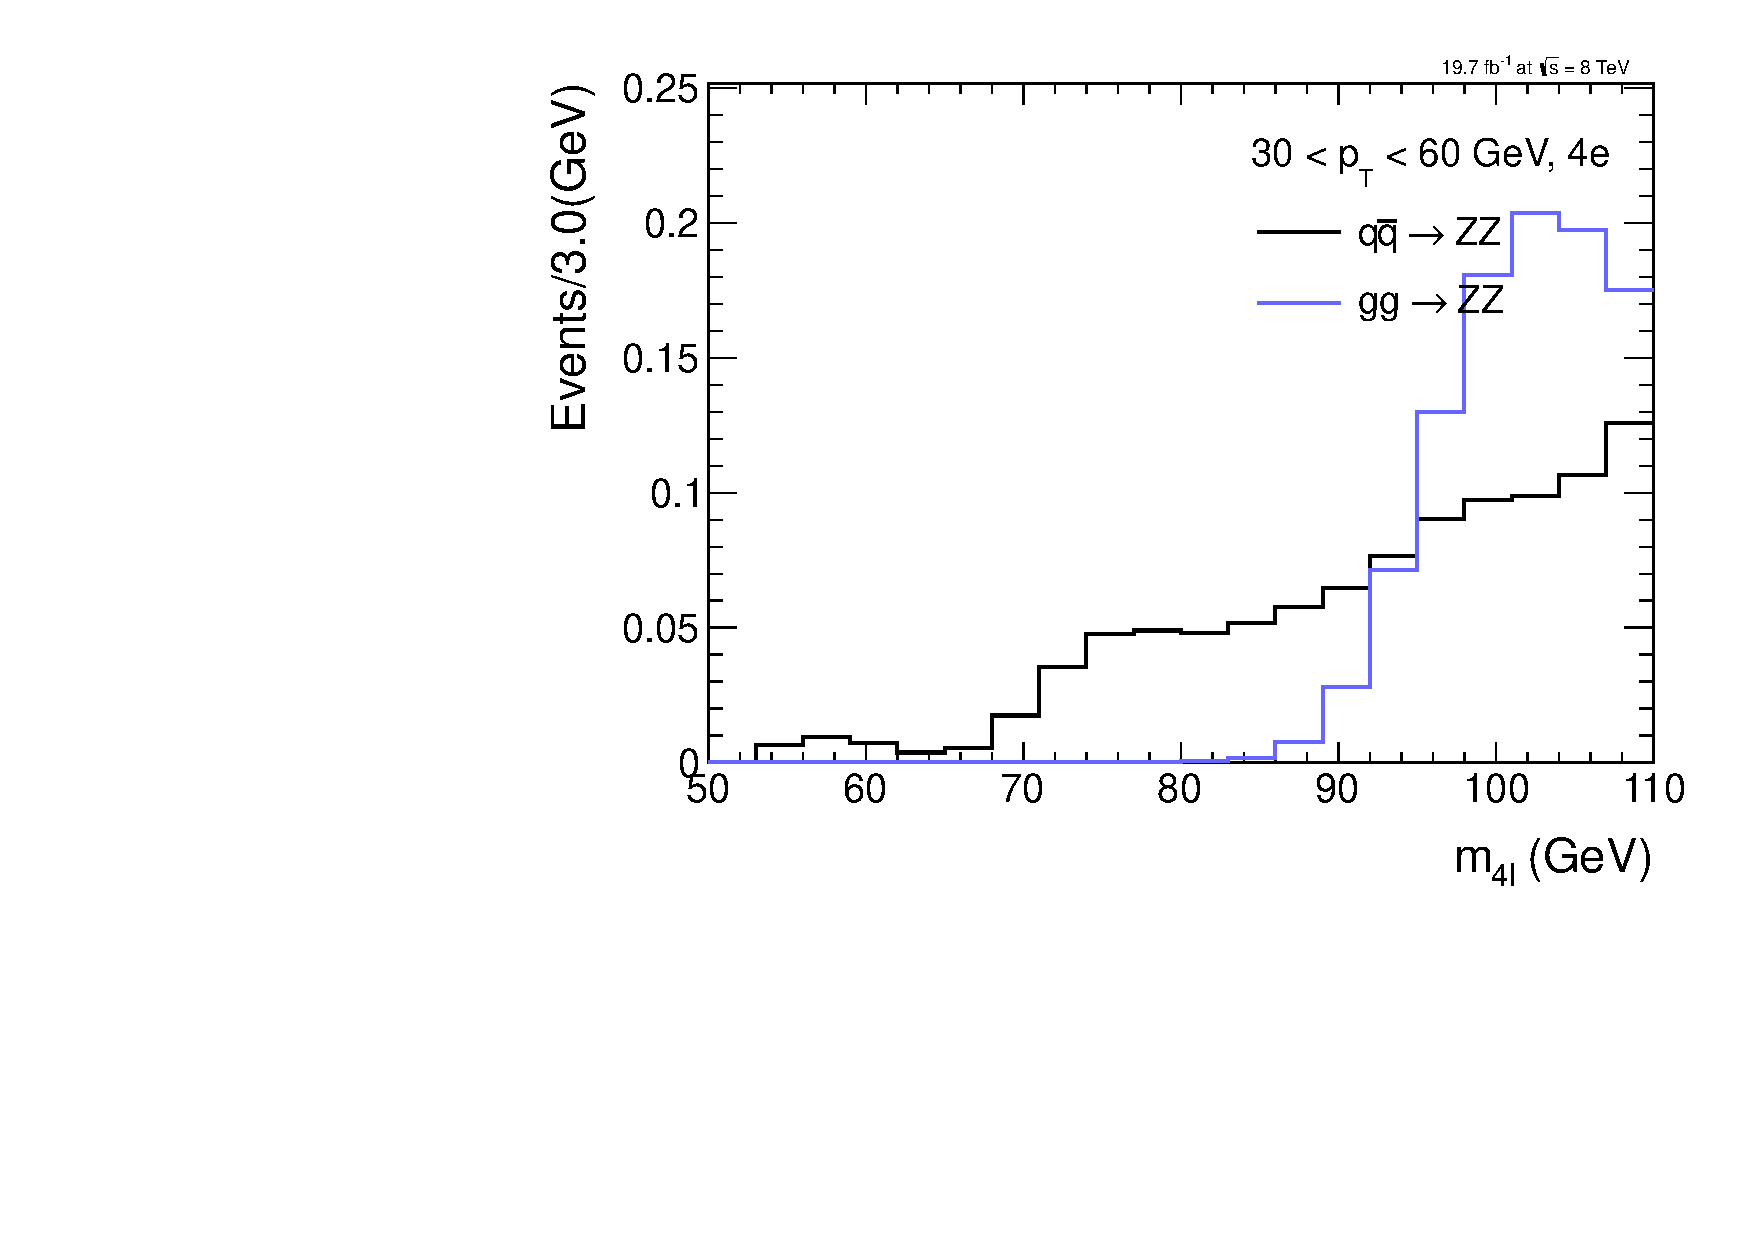
\includegraphics[width=0.32\textwidth,angle=0]{Appendix/figuresZ4l/XSTemplates_4e_pT4l_30_60_qqZZ_ggZZ.pdf}
      \label{fig:z4l_bkg-pT4l-qqZZ-ggZZ-4e:c}
    } \\
    
    \subfigure[$60.0 \GeV < \pt(4\ell) < 1000.0 \GeV$]{
      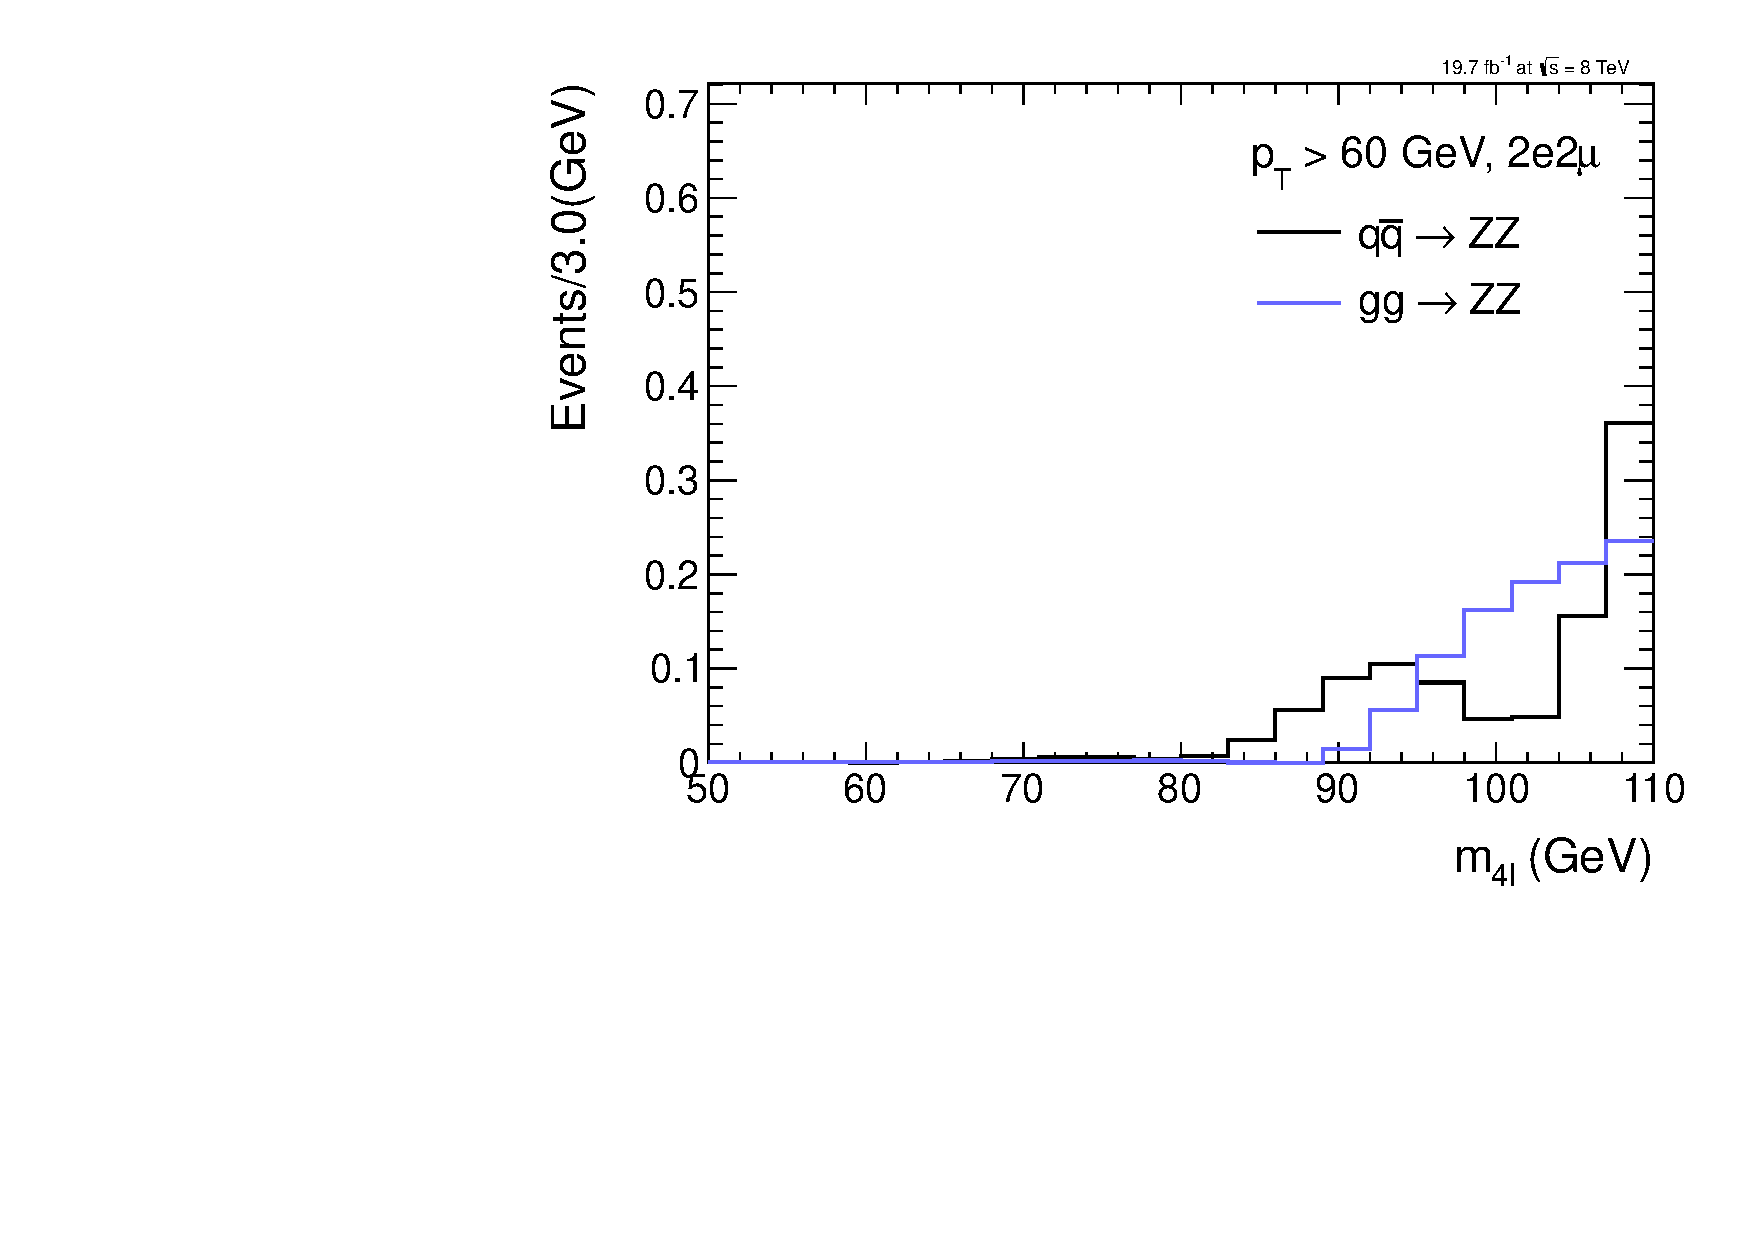
\includegraphics[width=0.32\textwidth,angle=0]{Appendix/figuresZ4l/XSTemplates_2e2mu_pT4l_60_1000_qqZZ_ggZZ.pdf}
      \label{fig:z4l_bkg-pT4l-qqZZ-ggZZ-2e2mu:d}
    }
    \subfigure[$60.0 \GeV < \pt(4\ell) < 1000.0 \GeV$]{
      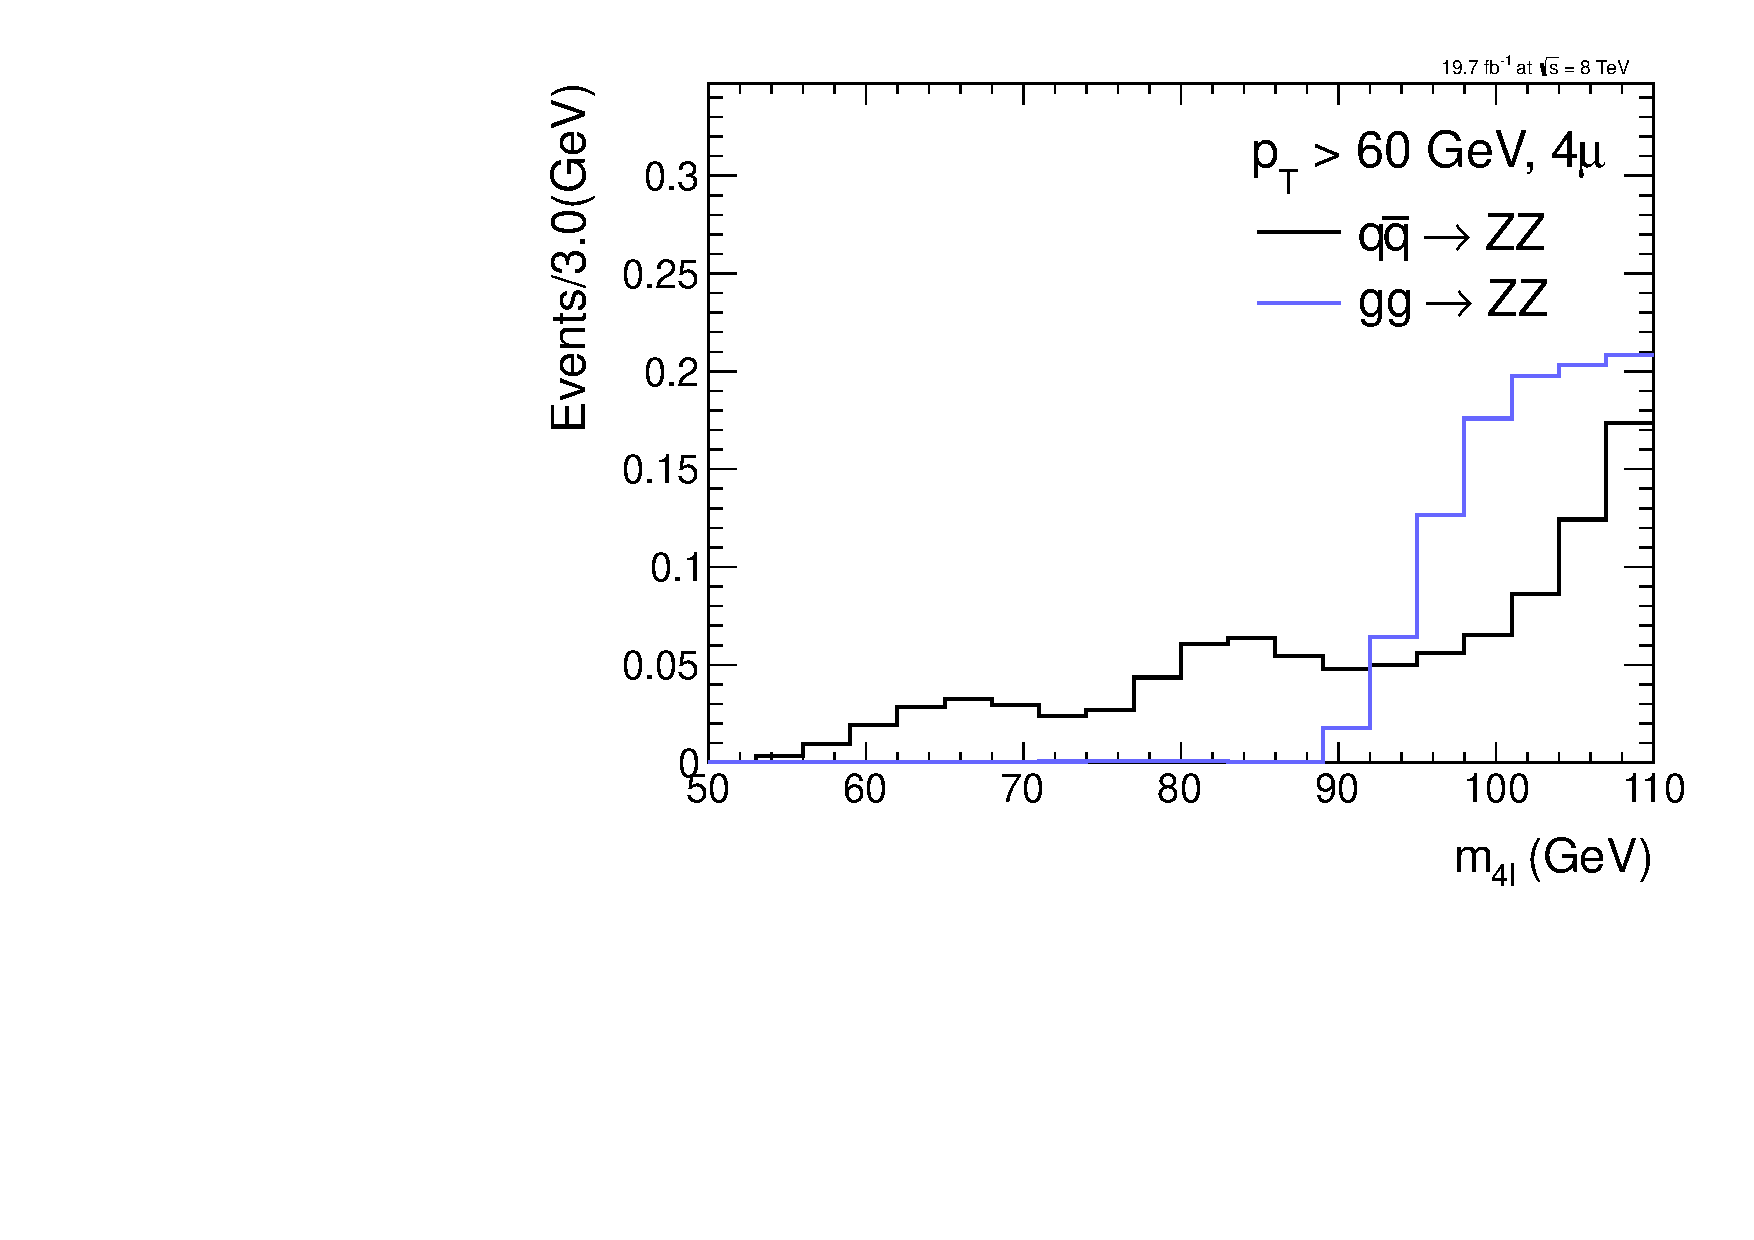
\includegraphics[width=0.32\textwidth,angle=0]{Appendix/figuresZ4l/XSTemplates_4mu_pT4l_60_1000_qqZZ_ggZZ.pdf}
      \label{fig:z4l_bkg-pT4l-qqZZ-ggZZ-4mu:d}
    }
    \subfigure[$60.0 \GeV < \pt(4\ell) < 1000.0 \GeV$]{
      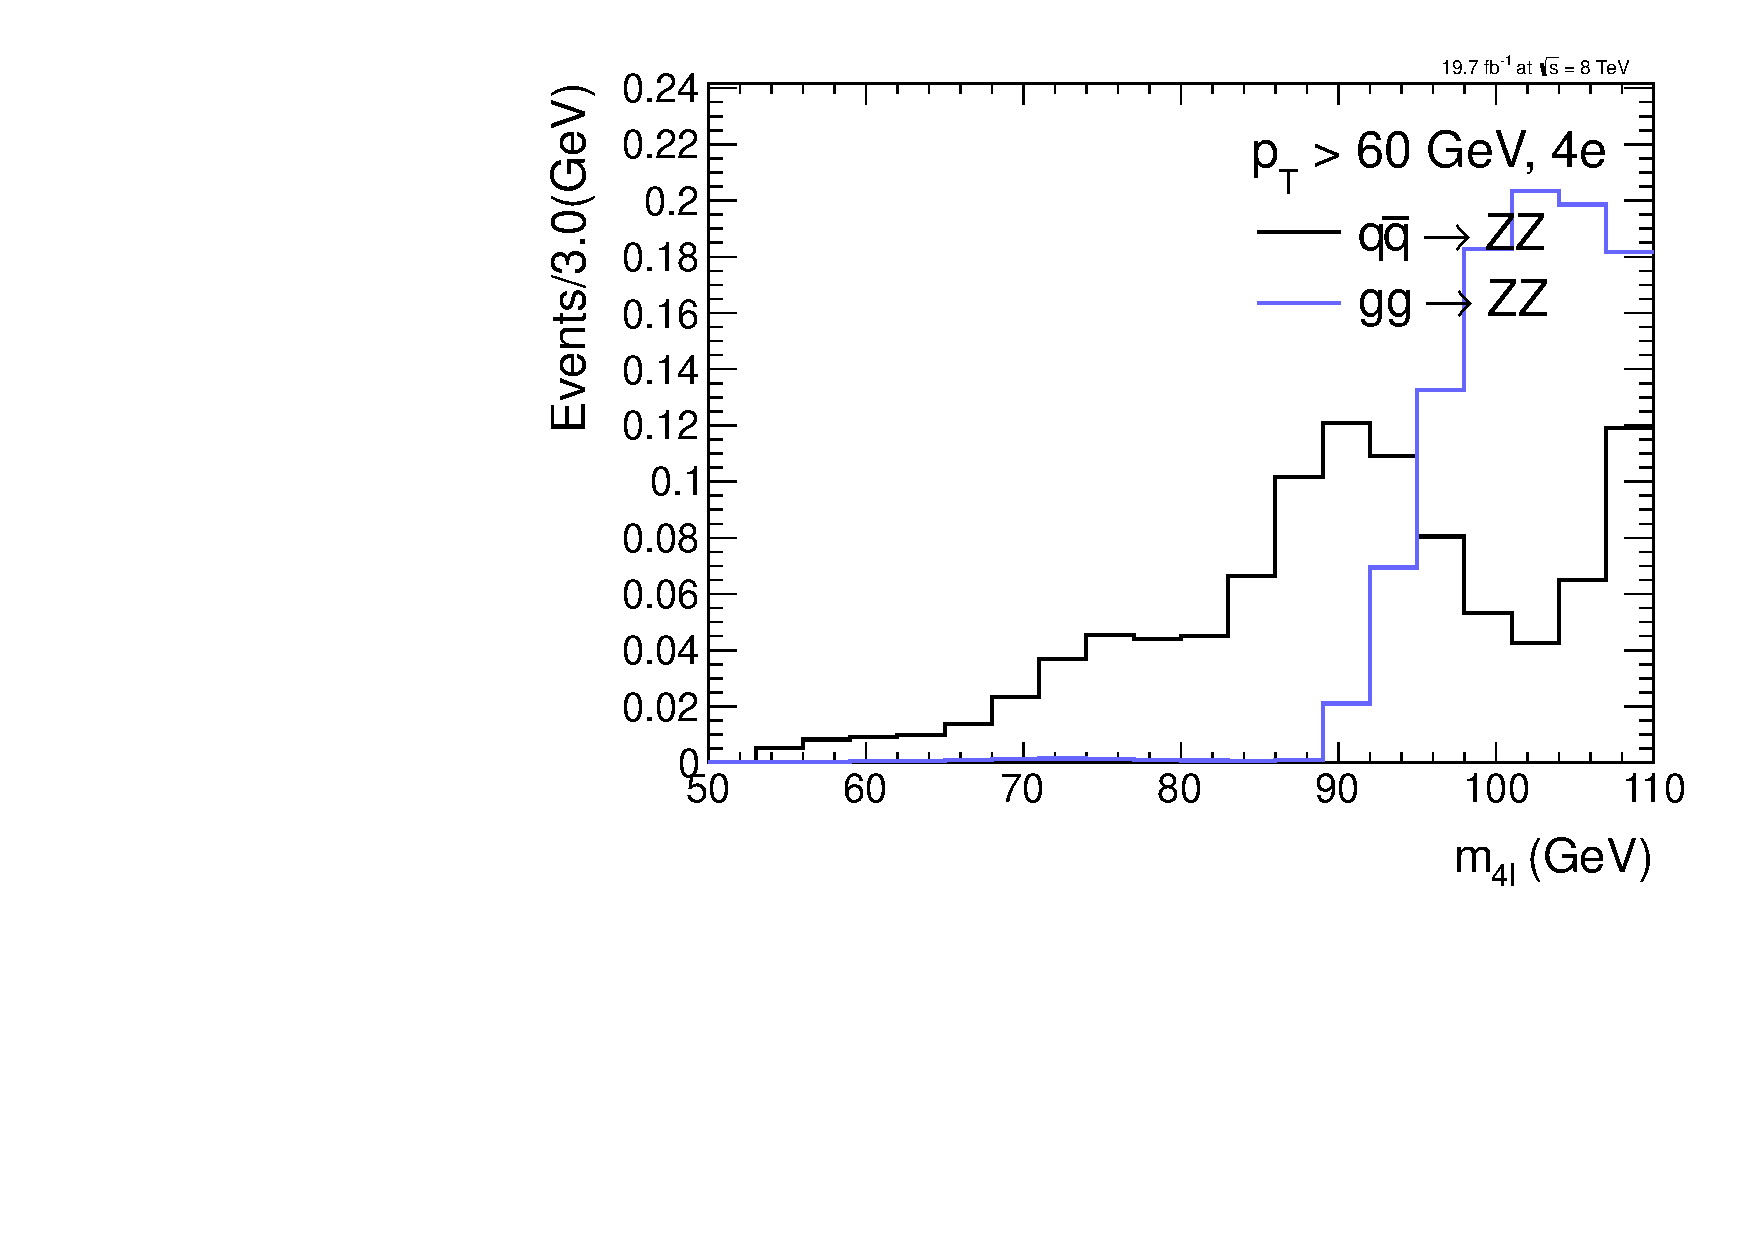
\includegraphics[width=0.32\textwidth,angle=0]{Appendix/figuresZ4l/XSTemplates_4e_pT4l_60_1000_qqZZ_ggZZ.pdf}
      \label{fig:z4l_bkg-pT4l-qqZZ-ggZZ-4e:d}
    } \\
    
    \caption{ Distributions of m($4\ell$) for the $qq \rightarrow \mathrm{ZZ}$ and $gg \rightarrow \mathrm{ZZ}$ backgrounds 
    in different bins of $\pt(4\ell)$ 
for Z$\to$4l measurements
for three final states: $2e2\mu$(left), $4\mu$(middle) and $4e$(right).}
  \label{fig:z4l_bkg-pT4l-qqZZ-ggZZ}
  
 \end{center}
\end{figure} 

\clearpage

\subsection{Background shapes in bins of $m(\mathrm{Z}_{2})$ }

\begin{figure}[!ht]
  \begin{center}
  
    \subfigure[$12.0 \GeV < \mathrm{m}(\mathrm{Z}_{2}) < 20.0 \GeV$]{
      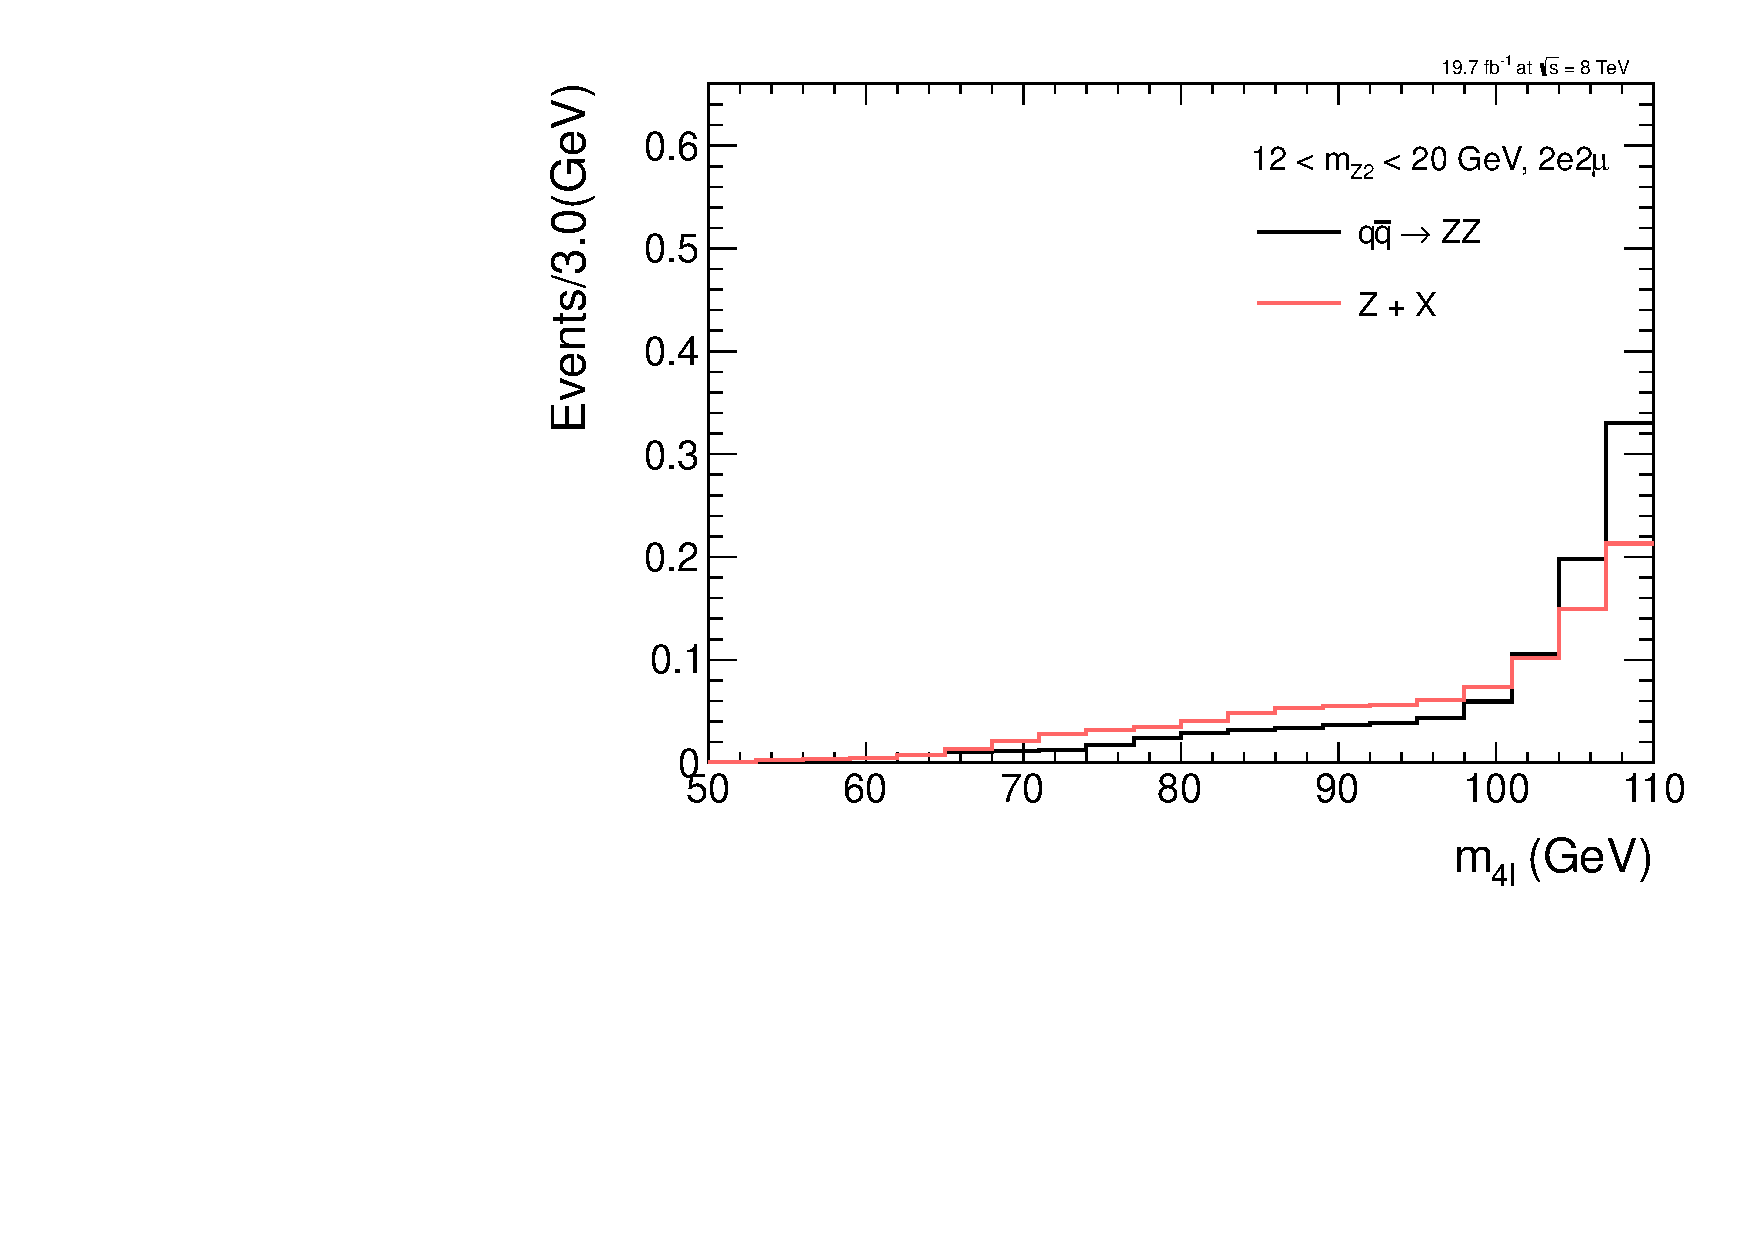
\includegraphics[width=0.32\textwidth,angle=0]{Appendix/figuresZ4l/XSTemplates_2e2mu_massZ2_12_20_qqZZ_ZJetsCR.pdf}
      \label{fig:z4l_bkg-massZ2-qqZZ-ZX-2e2mu:a}
    }    
    \subfigure[$12.0 \GeV < \mathrm{m}(\mathrm{Z}_{2}) < 20.0 \GeV$]{
      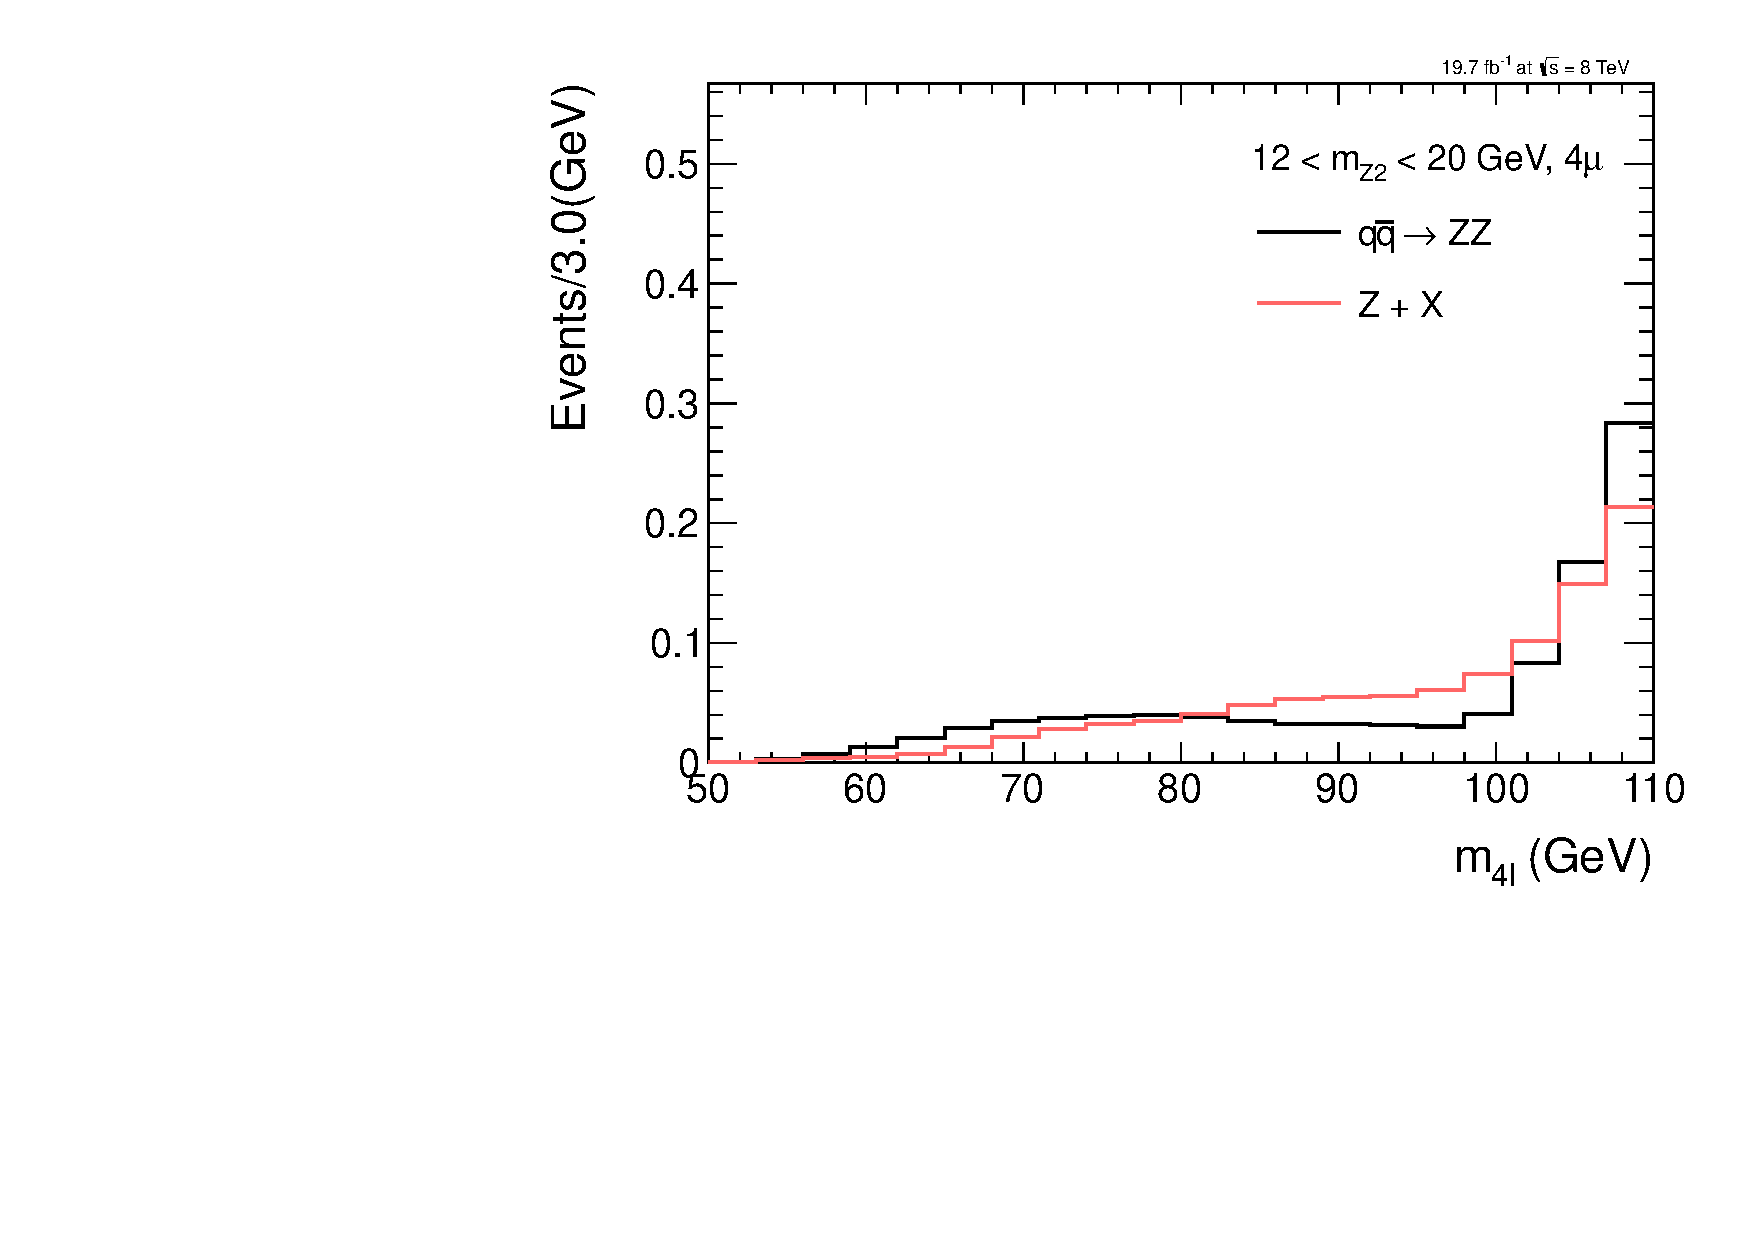
\includegraphics[width=0.32\textwidth,angle=0]{Appendix/figuresZ4l/XSTemplates_4mu_massZ2_12_20_qqZZ_ZJetsCR.pdf}
      \label{fig:z4l_bkg-massZ2-qqZZ-ZX-4mu:a}
    }    
    \subfigure[$12.0 \GeV < \mathrm{m}(\mathrm{Z}_{2}) < 20.0 \GeV$]{
      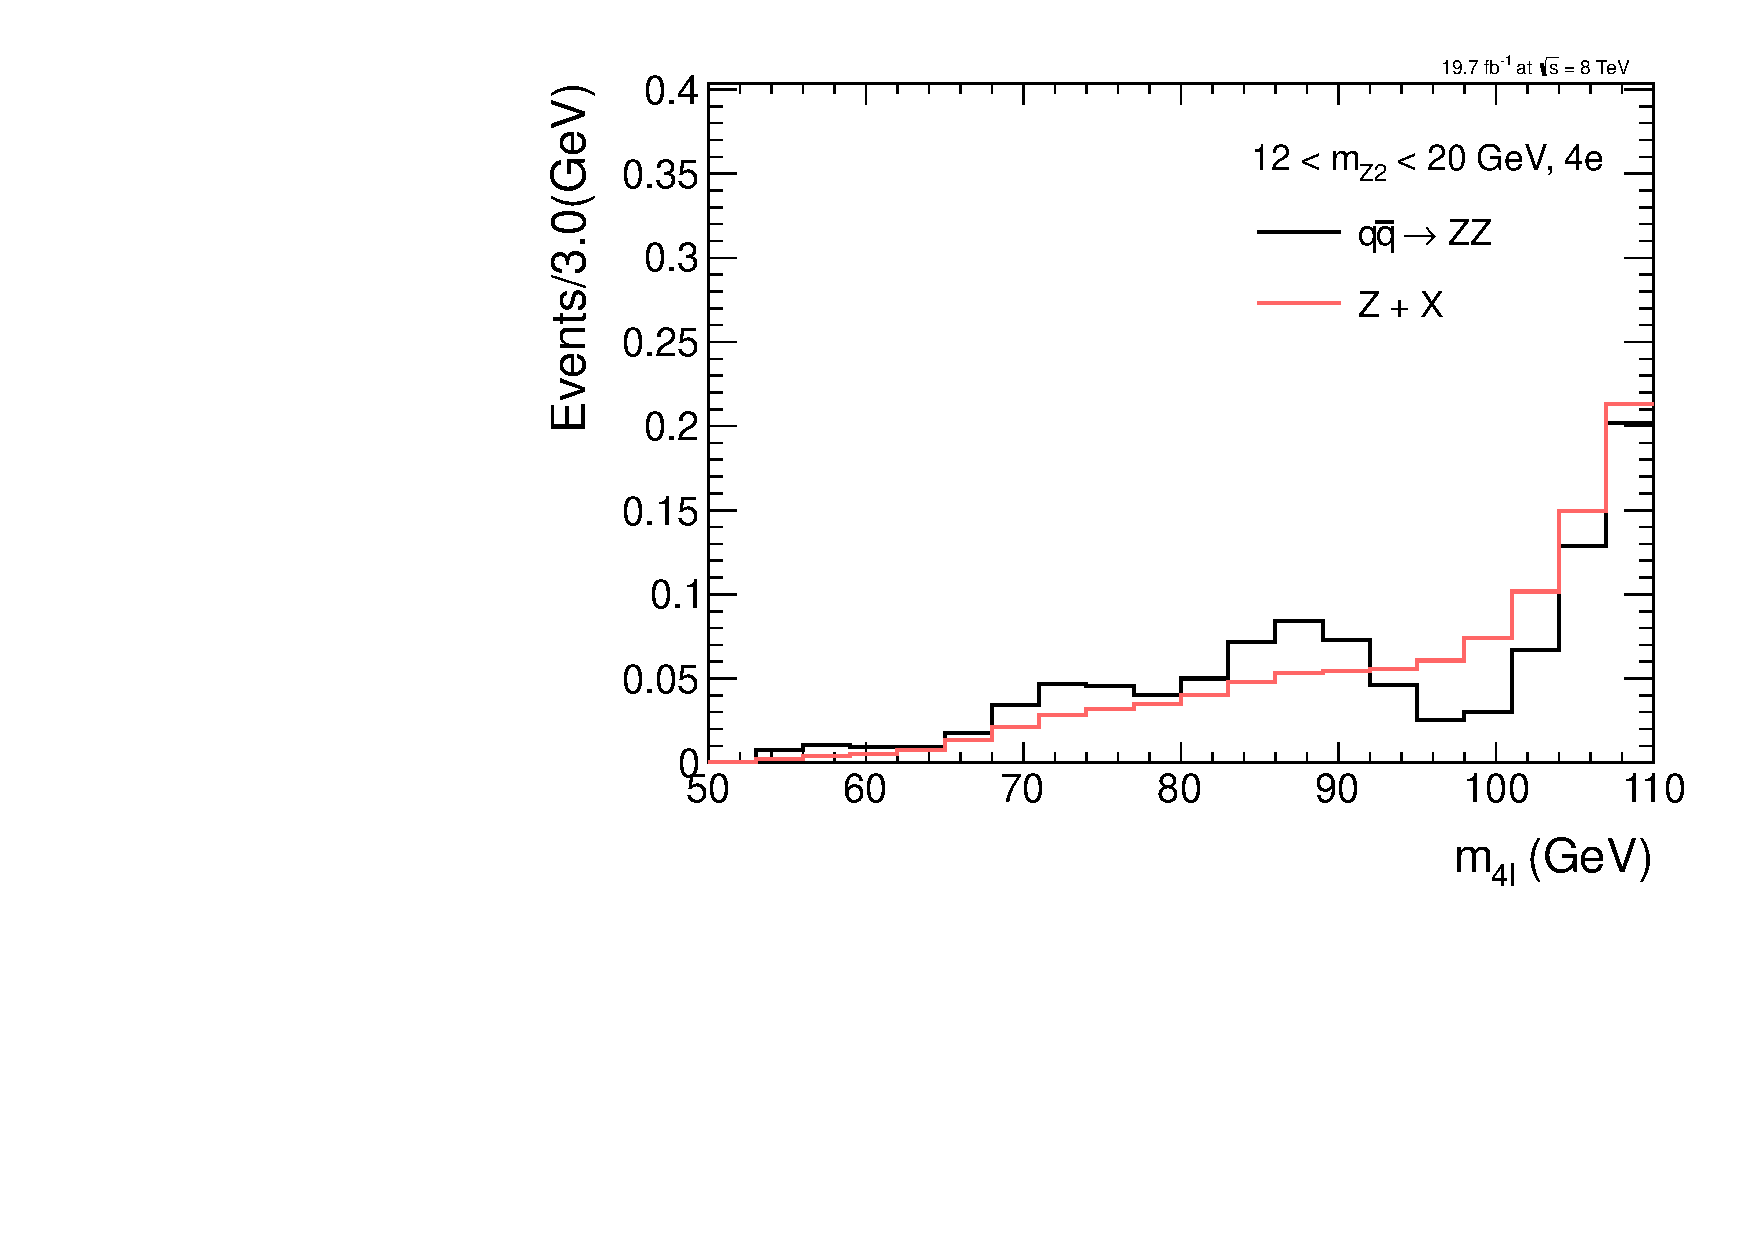
\includegraphics[width=0.32\textwidth,angle=0]{Appendix/figuresZ4l/XSTemplates_4e_massZ2_12_20_qqZZ_ZJetsCR.pdf}
      \label{fig:z4l_bkg-massZ2-qqZZ-ZX-4e:a}
    }    \\

    \subfigure[$20.0 \GeV < \mathrm{m}(\mathrm{Z}_{2}) < 28.0 \GeV$]{
      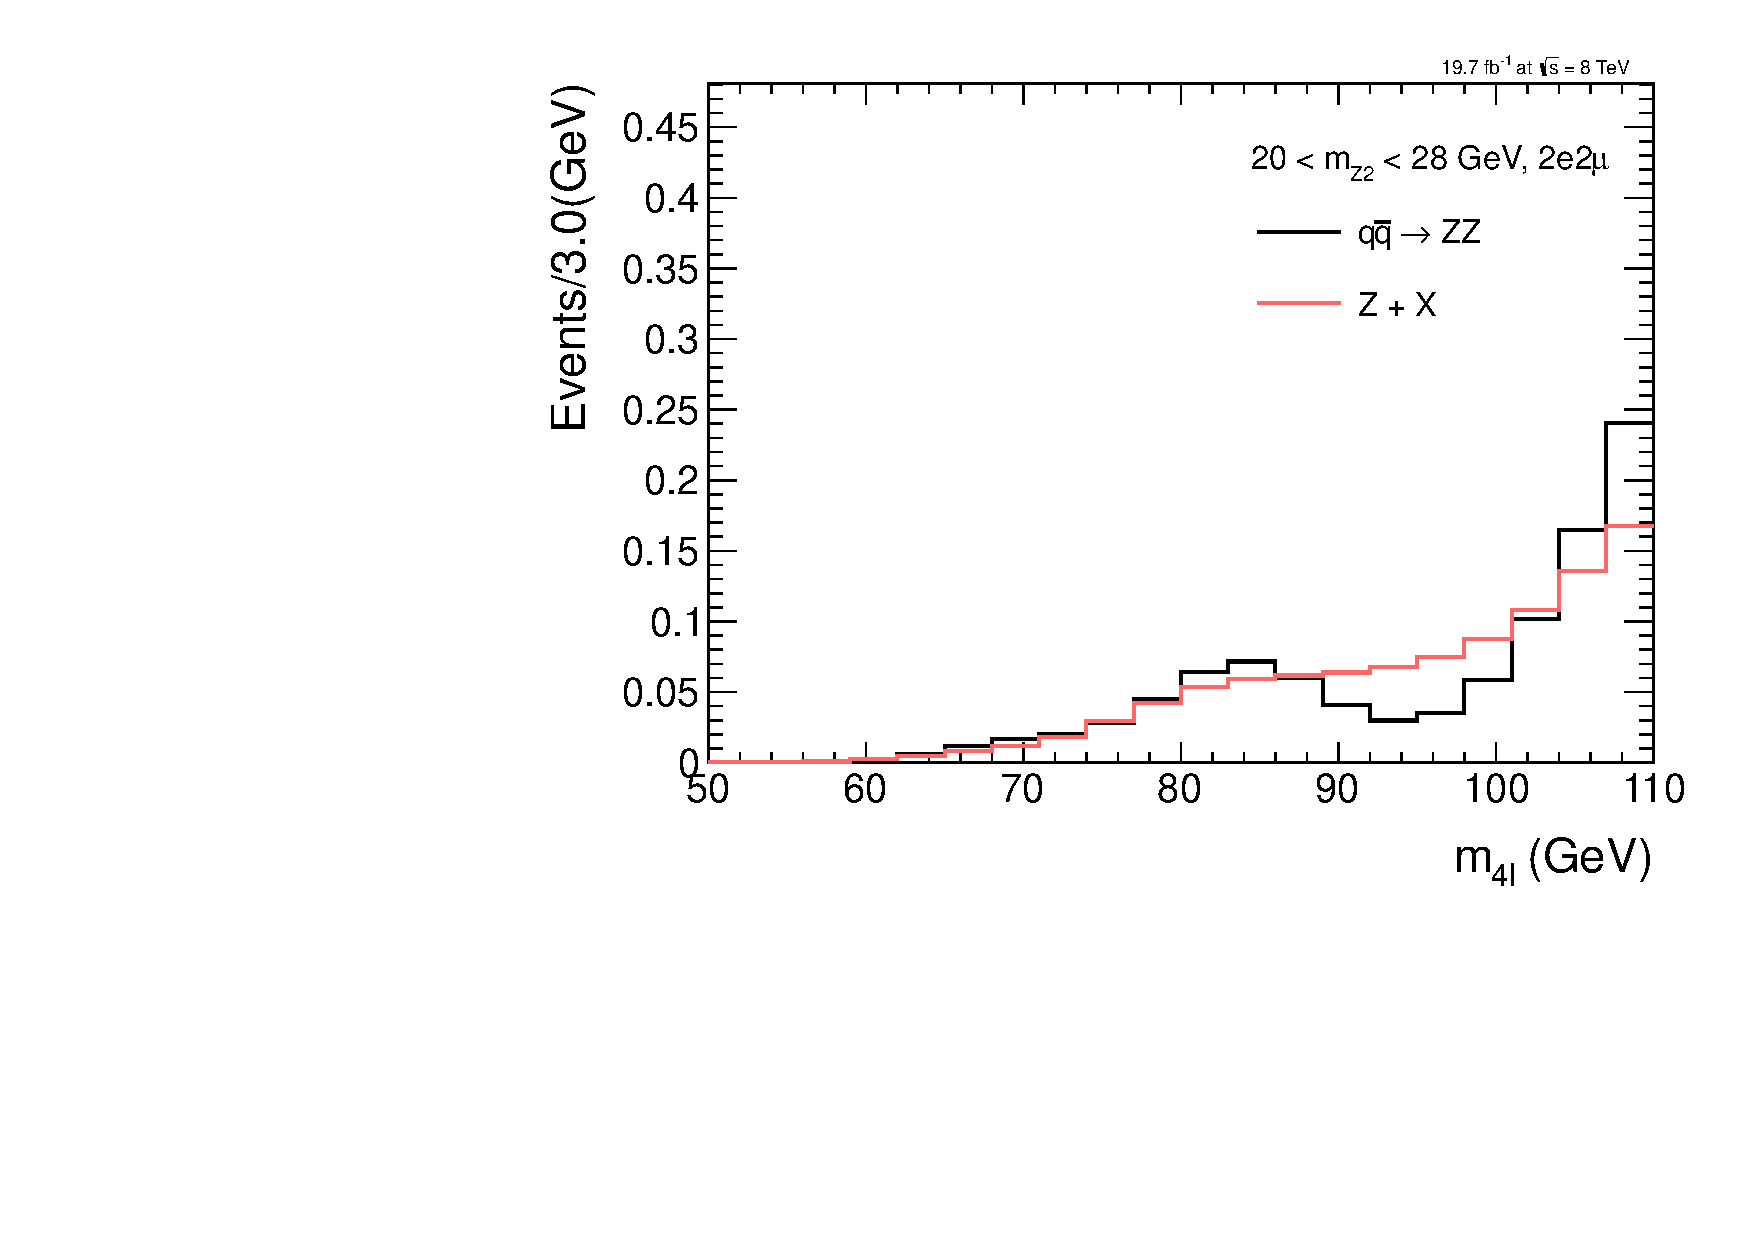
\includegraphics[width=0.32\textwidth,angle=0]{Appendix/figuresZ4l/XSTemplates_2e2mu_massZ2_20_28_qqZZ_ZJetsCR.pdf}
      \label{fig:z4l_bkg-massZ2-qqZZ-ZX-2e2mu:b}
    }
    \subfigure[$20.0 \GeV < \mathrm{m}(\mathrm{Z}_{2}) < 28.0 \GeV$]{
      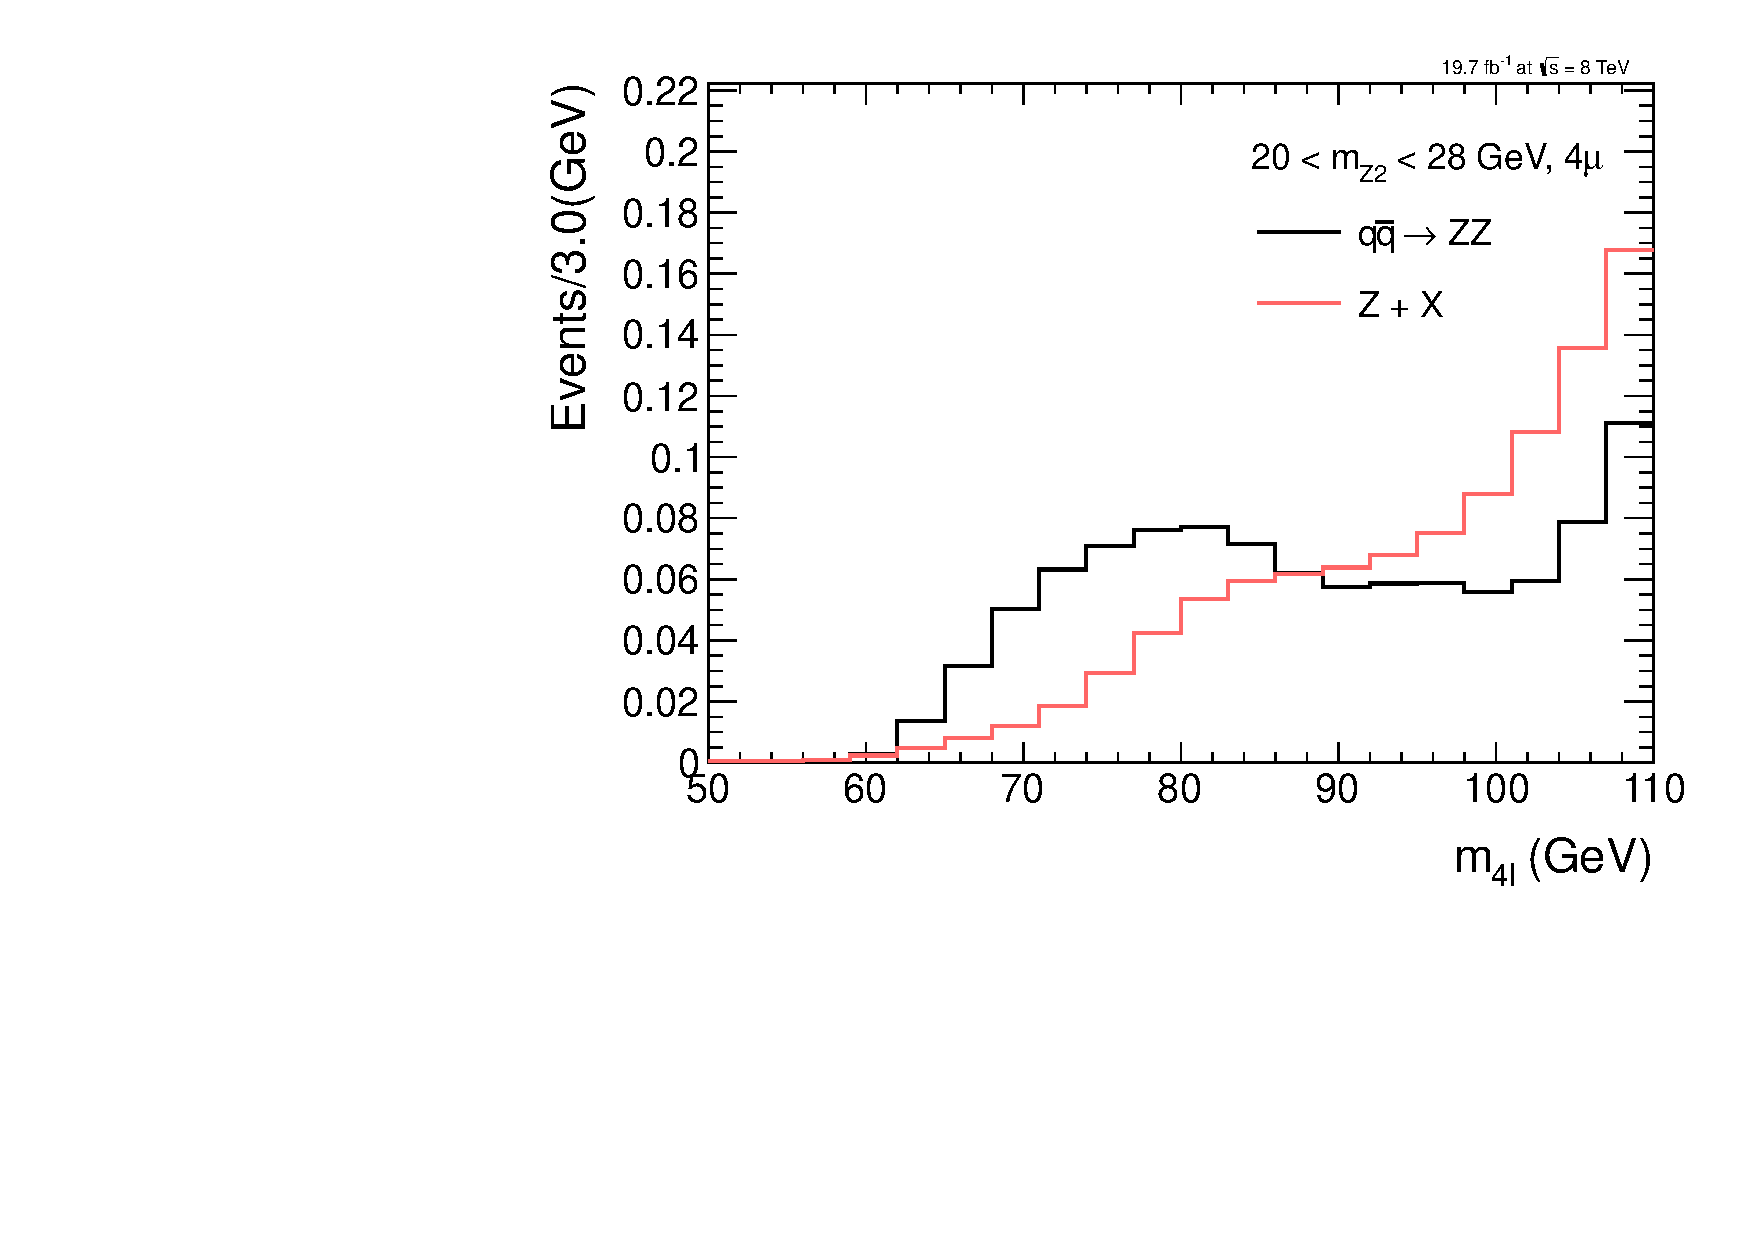
\includegraphics[width=0.32\textwidth,angle=0]{Appendix/figuresZ4l/XSTemplates_4mu_massZ2_20_28_qqZZ_ZJetsCR.pdf}
      \label{fig:z4l_bkg-massZ2-qqZZ-ZX-4mu:b}
    } 
    \subfigure[$20.0 \GeV < \mathrm{m}(\mathrm{Z}_{2}) < 28.0 \GeV$]{
      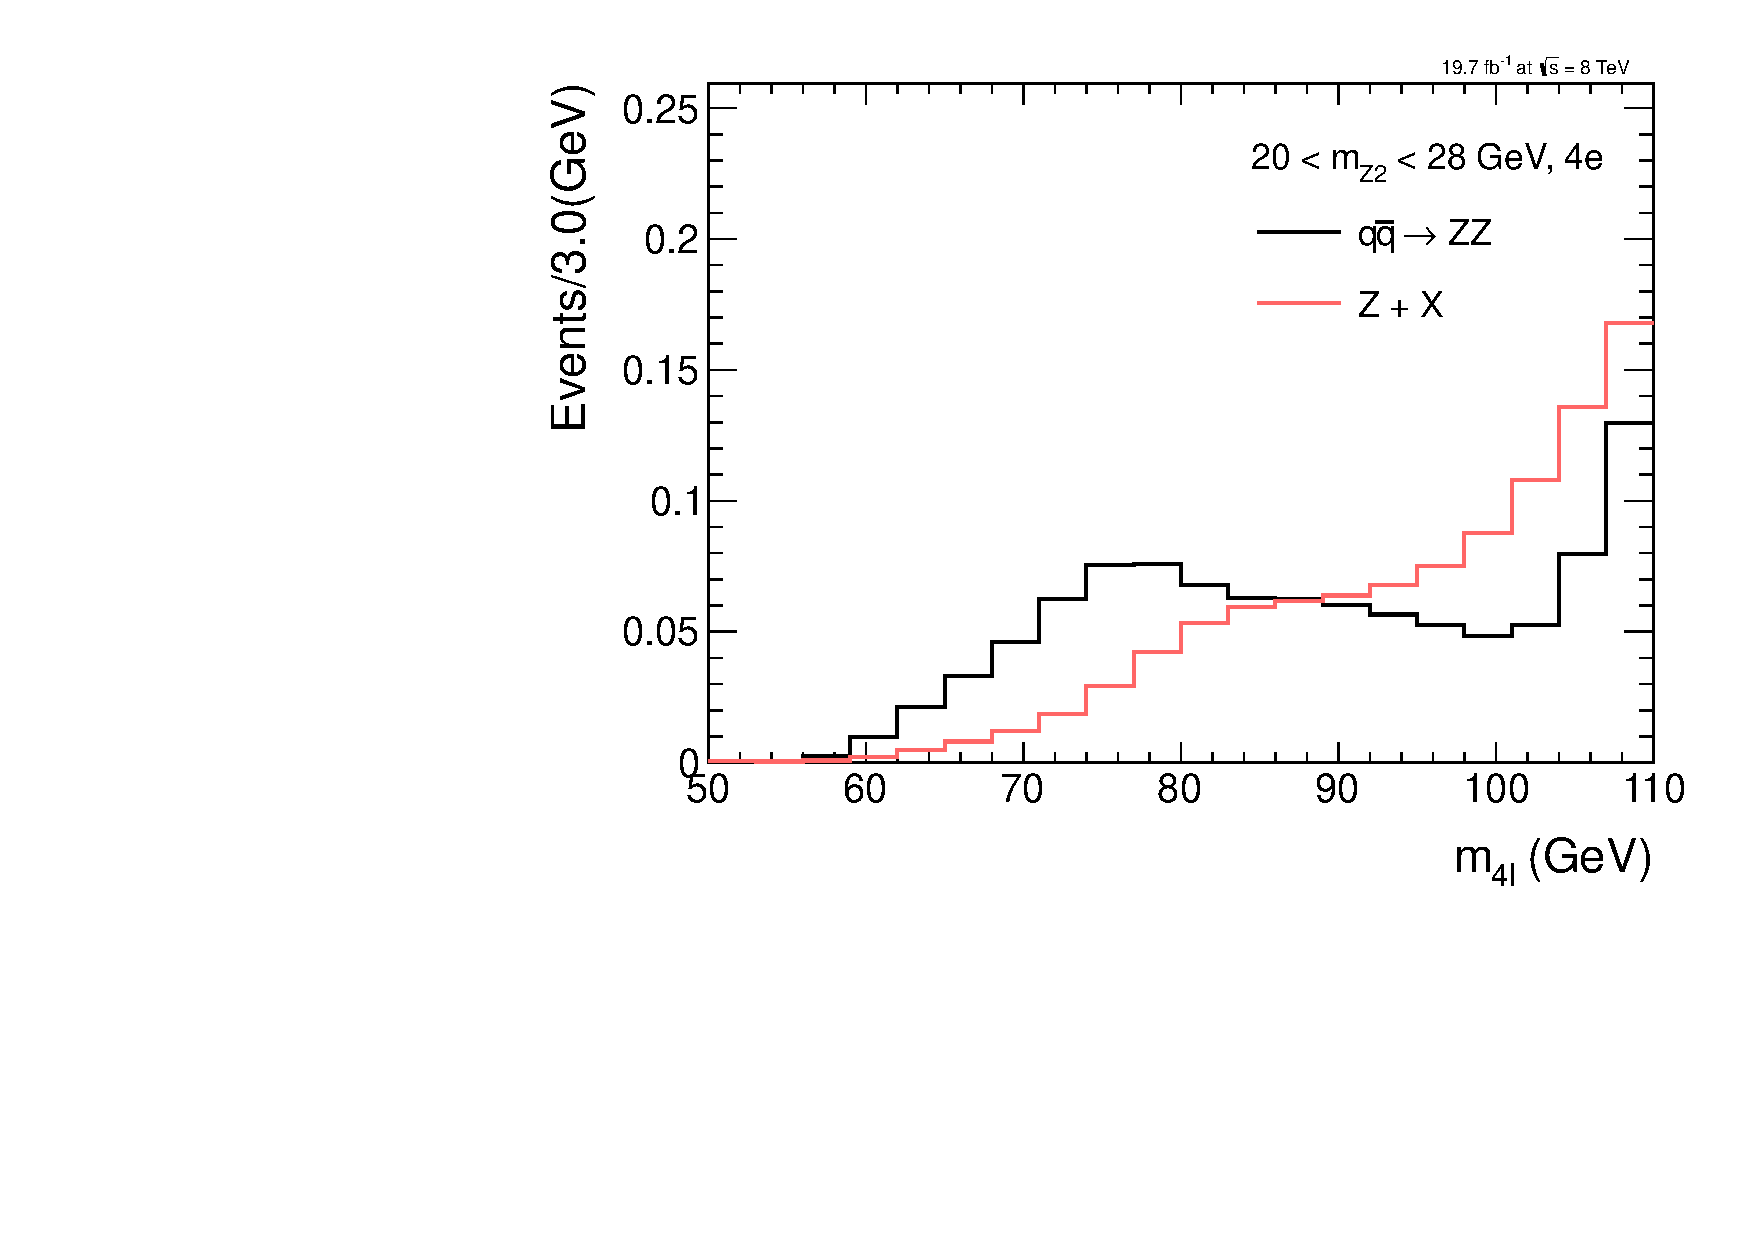
\includegraphics[width=0.32\textwidth,angle=0]{Appendix/figuresZ4l/XSTemplates_4e_massZ2_20_28_qqZZ_ZJetsCR.pdf}
      \label{fig:z4l_bkg-massZ2-qqZZ-ZX-4e:b}
    } \\
    
    \subfigure[$28.0 \GeV < \mathrm{m}(\mathrm{Z}_{2}) < 35.0 \GeV$]{
      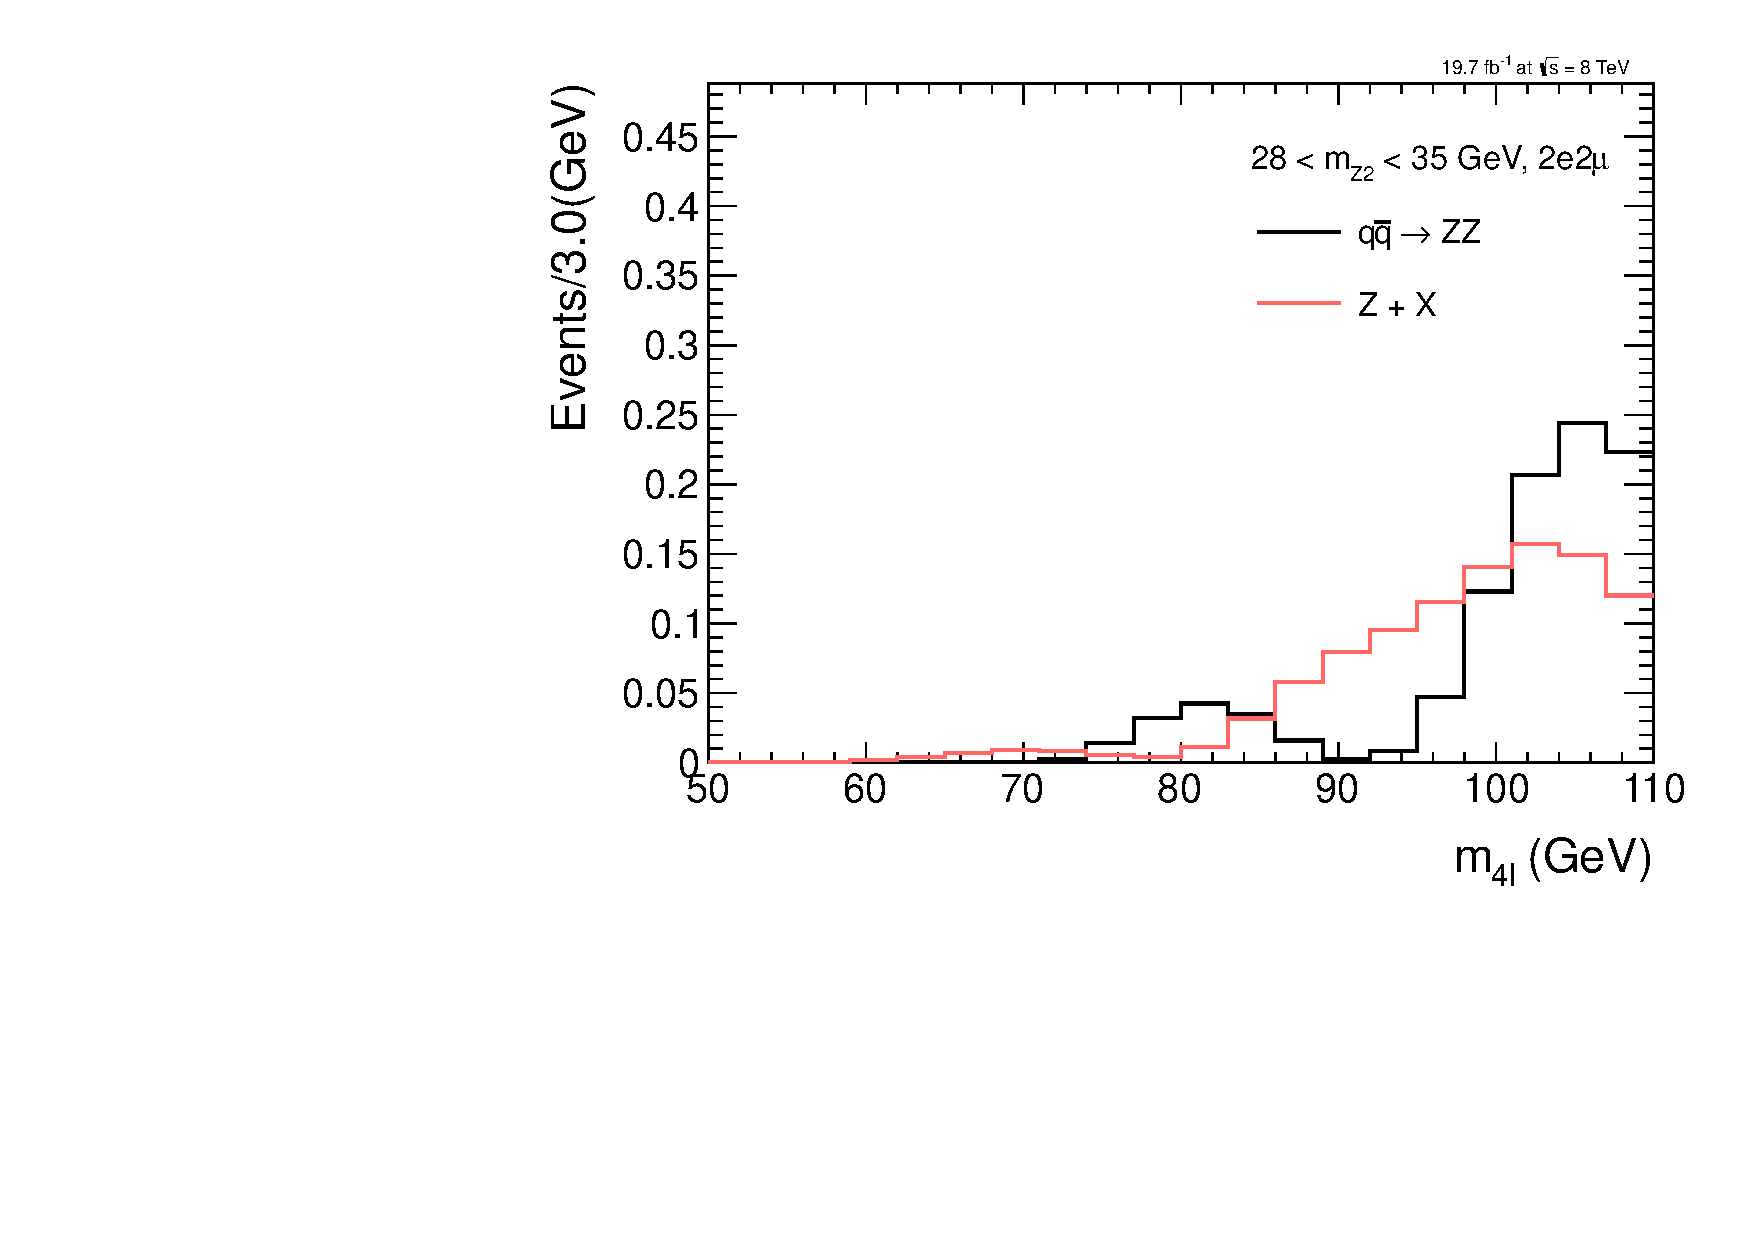
\includegraphics[width=0.32\textwidth,angle=0]{Appendix/figuresZ4l/XSTemplates_2e2mu_massZ2_28_35_qqZZ_ZJetsCR.pdf}
      \label{fig:z4l_bkg-massZ2-qqZZ-ZX-2e2mu:c}
    }
    \subfigure[$28.0 \GeV < \mathrm{m}(\mathrm{Z}_{2}) < 35.0 \GeV$]{
      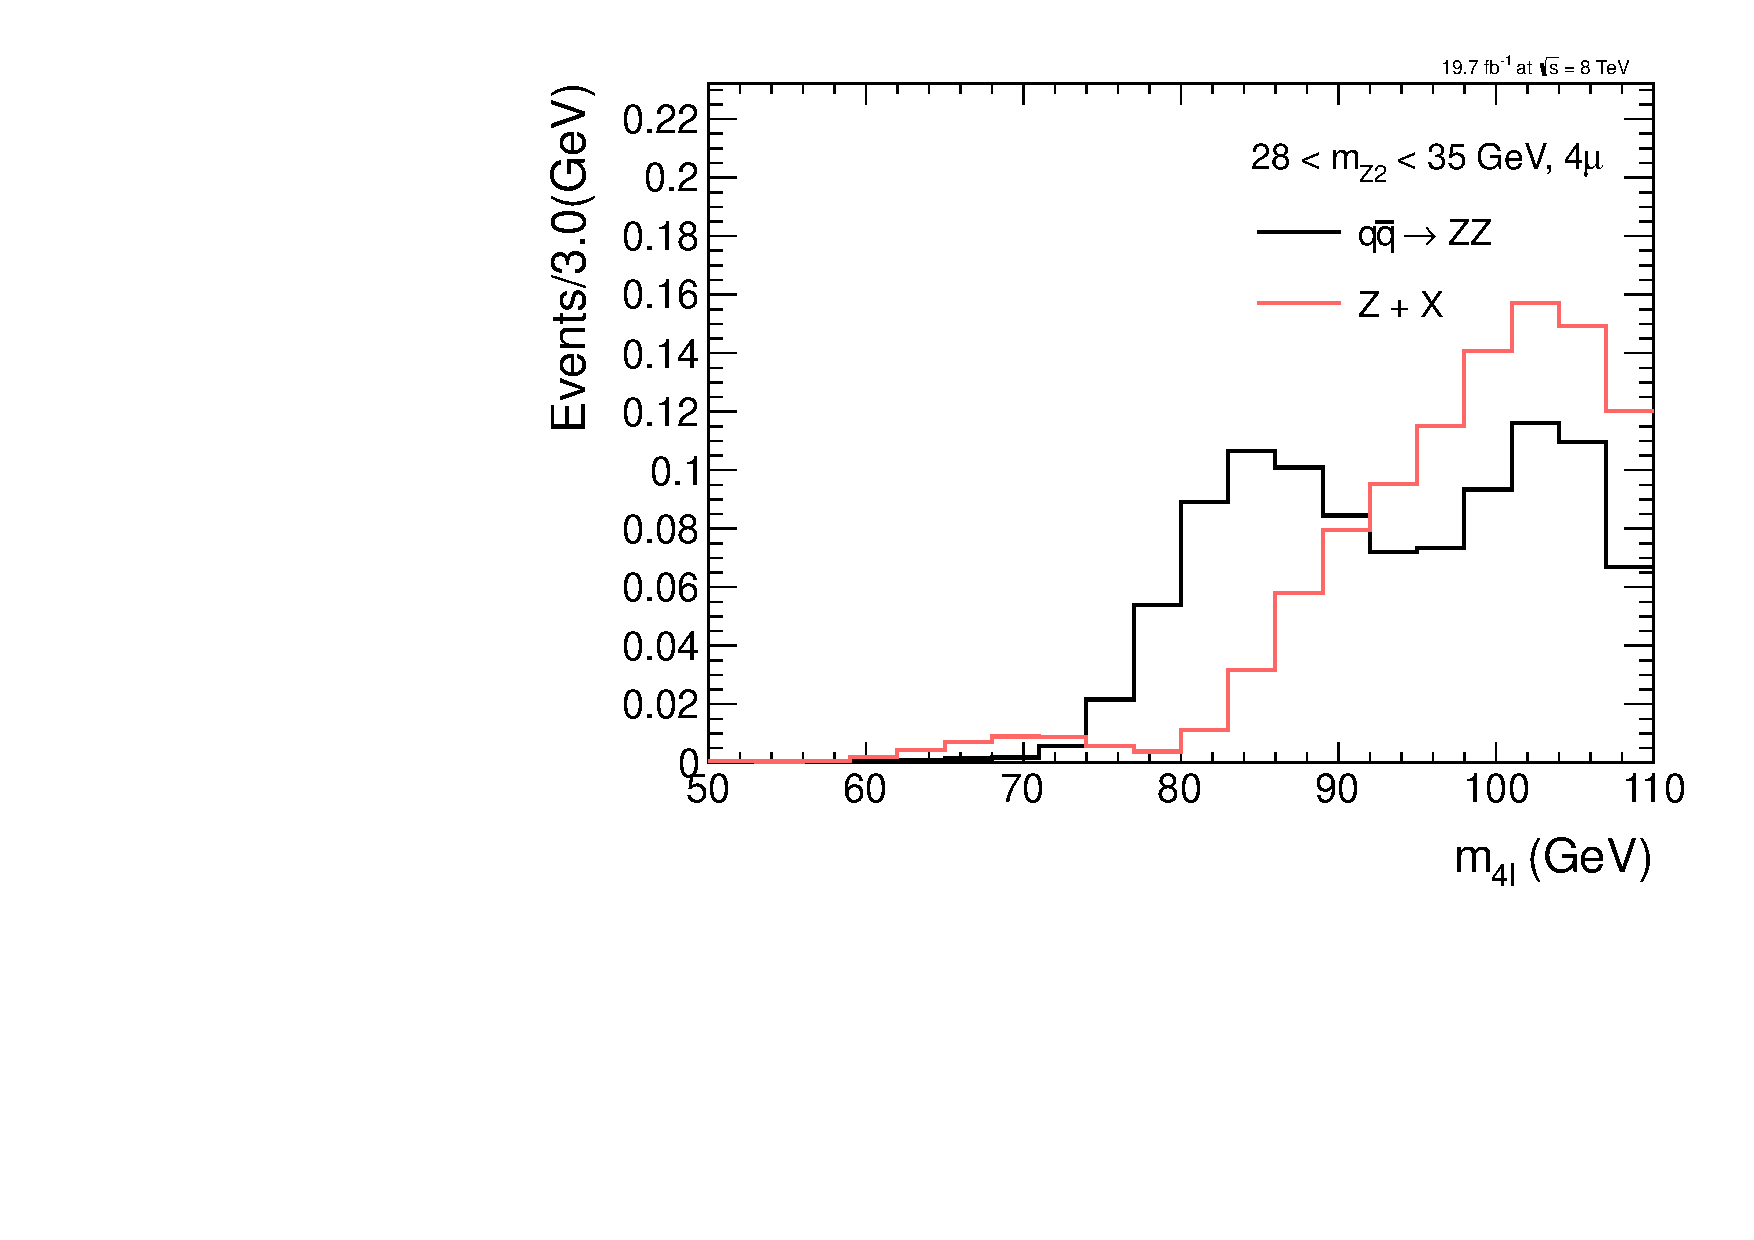
\includegraphics[width=0.32\textwidth,angle=0]{Appendix/figuresZ4l/XSTemplates_4mu_massZ2_28_35_qqZZ_ZJetsCR.pdf}
      \label{fig:z4l_bkg-massZ2-qqZZ-ZX-4mu:c}
    }
    \subfigure[$28.0 \GeV < \mathrm{m}(\mathrm{Z}_{2}) < 35.0 \GeV$]{
      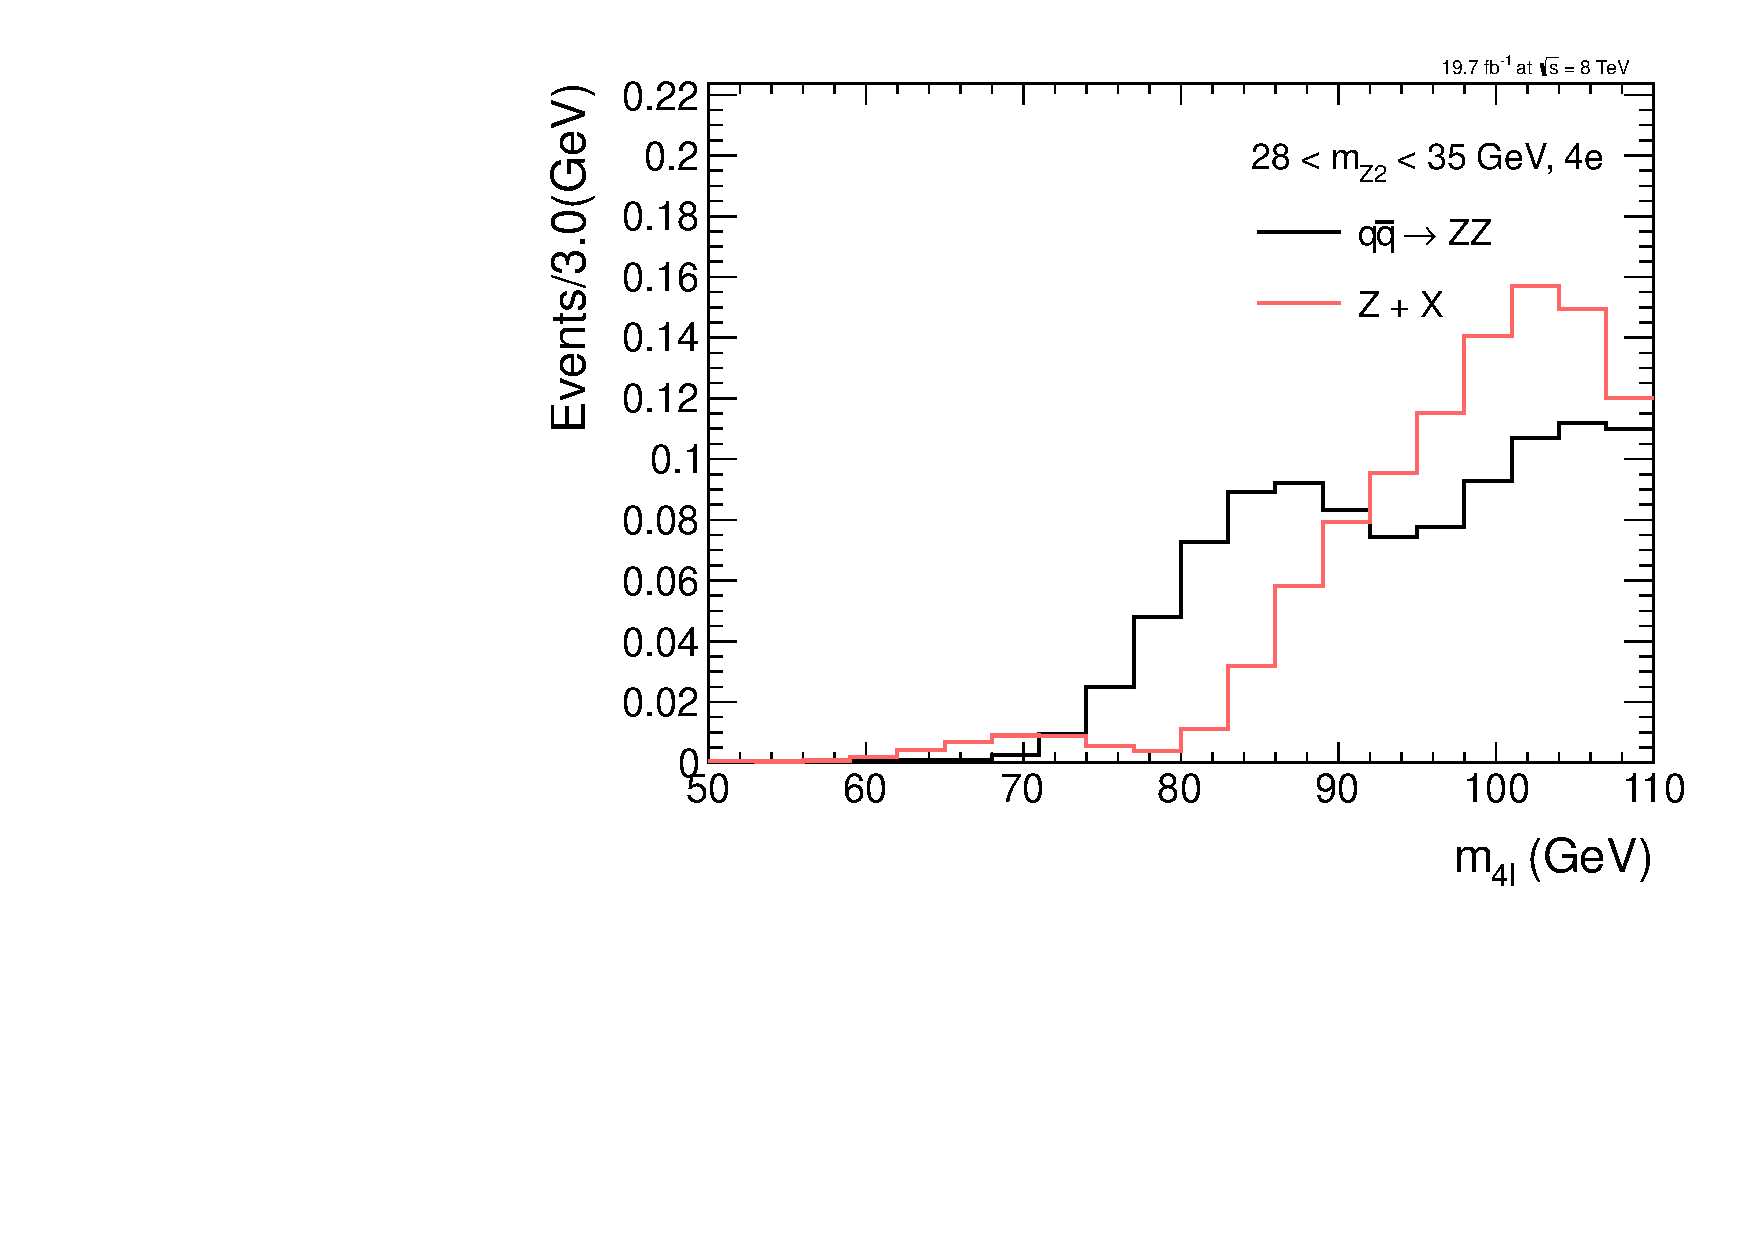
\includegraphics[width=0.32\textwidth,angle=0]{Appendix/figuresZ4l/XSTemplates_4e_massZ2_28_35_qqZZ_ZJetsCR.pdf}
      \label{fig:z4l_bkg-massZ2-qqZZ-ZX-4e:c}
    } \\
    
    \subfigure[$35.0 \GeV < \mathrm{m}(\mathrm{Z}_{2}) < 120.0 \GeV$]{
      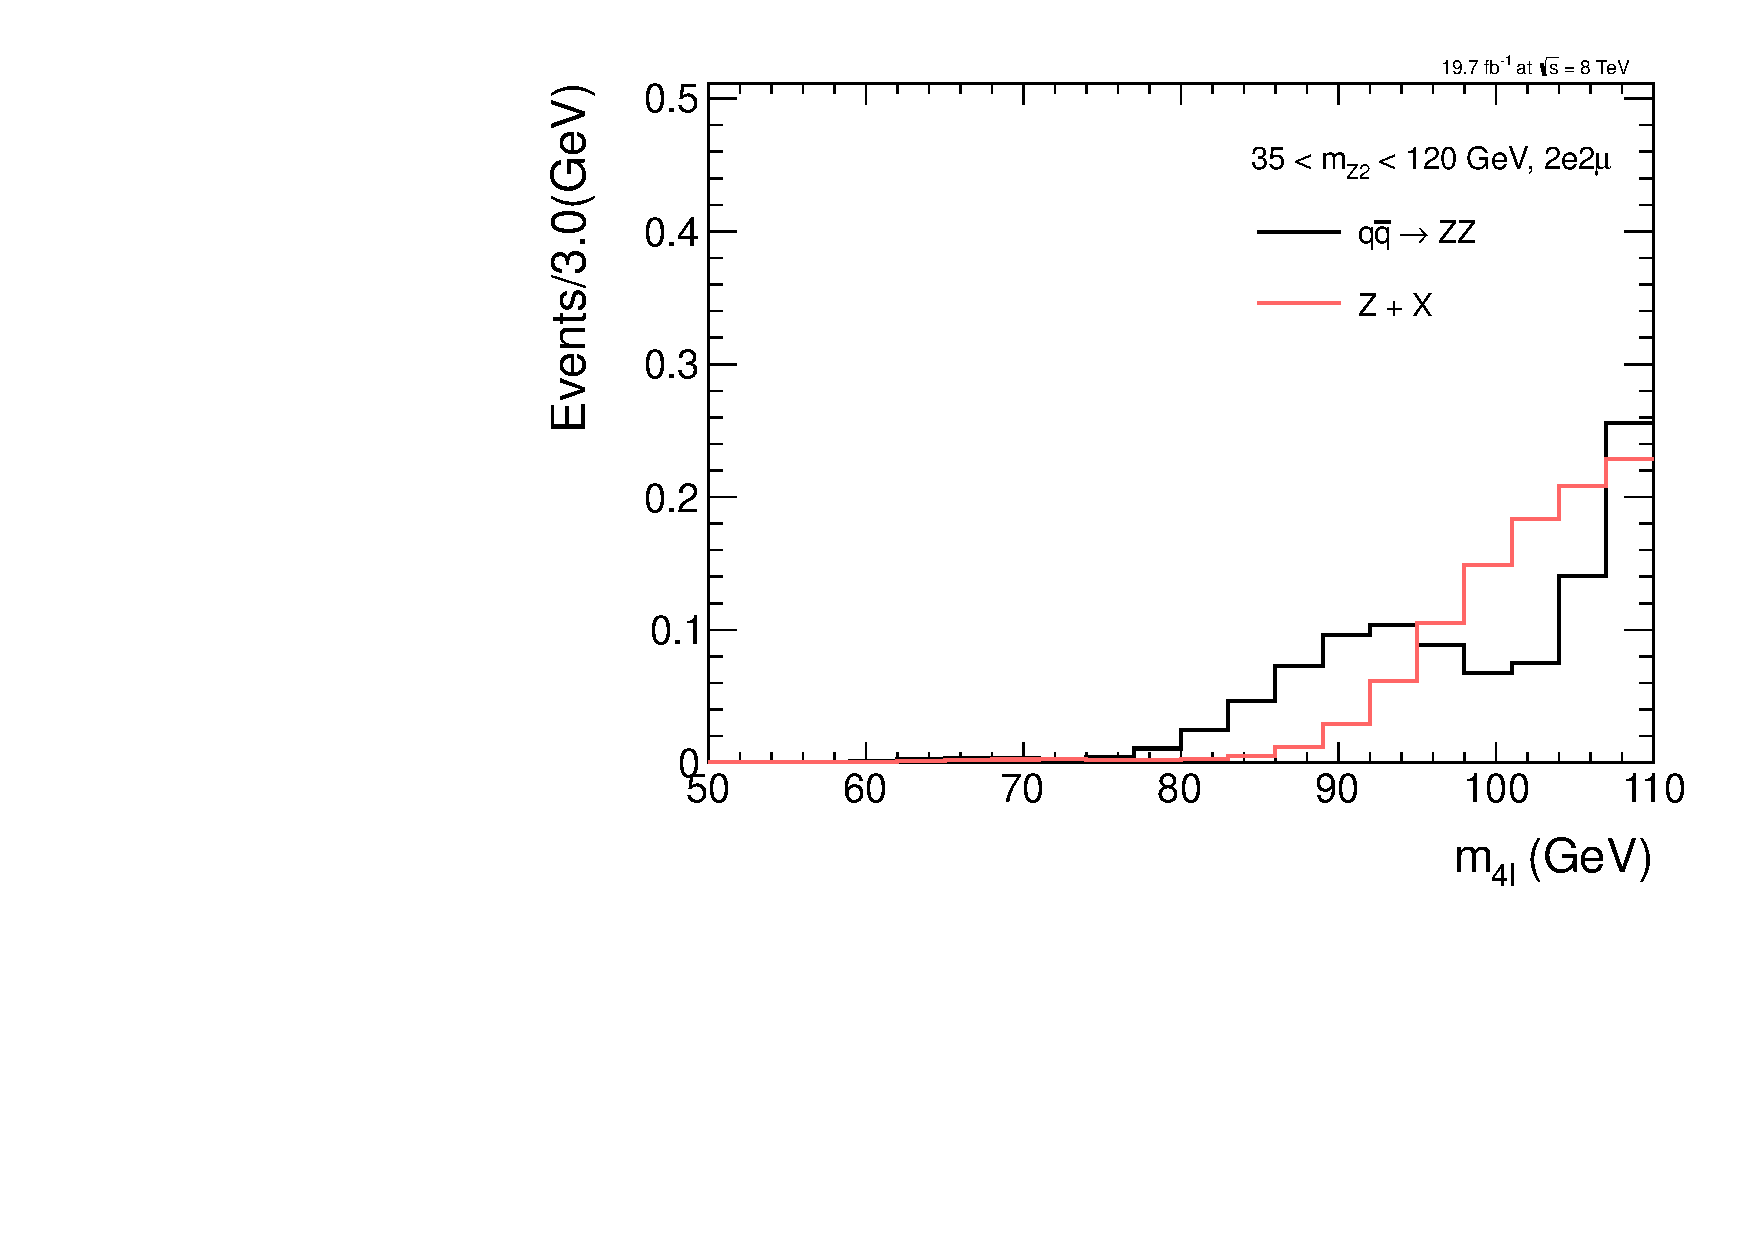
\includegraphics[width=0.32\textwidth,angle=0]{Appendix/figuresZ4l/XSTemplates_2e2mu_massZ2_35_120_qqZZ_ZJetsCR.pdf}
      \label{fig:z4l_bkg-massZ2-qqZZ-ZX-2e2mu:d}
    }
    \subfigure[$35.0 \GeV < \mathrm{m}(\mathrm{Z}_{2}) < 120.0 \GeV$]{
      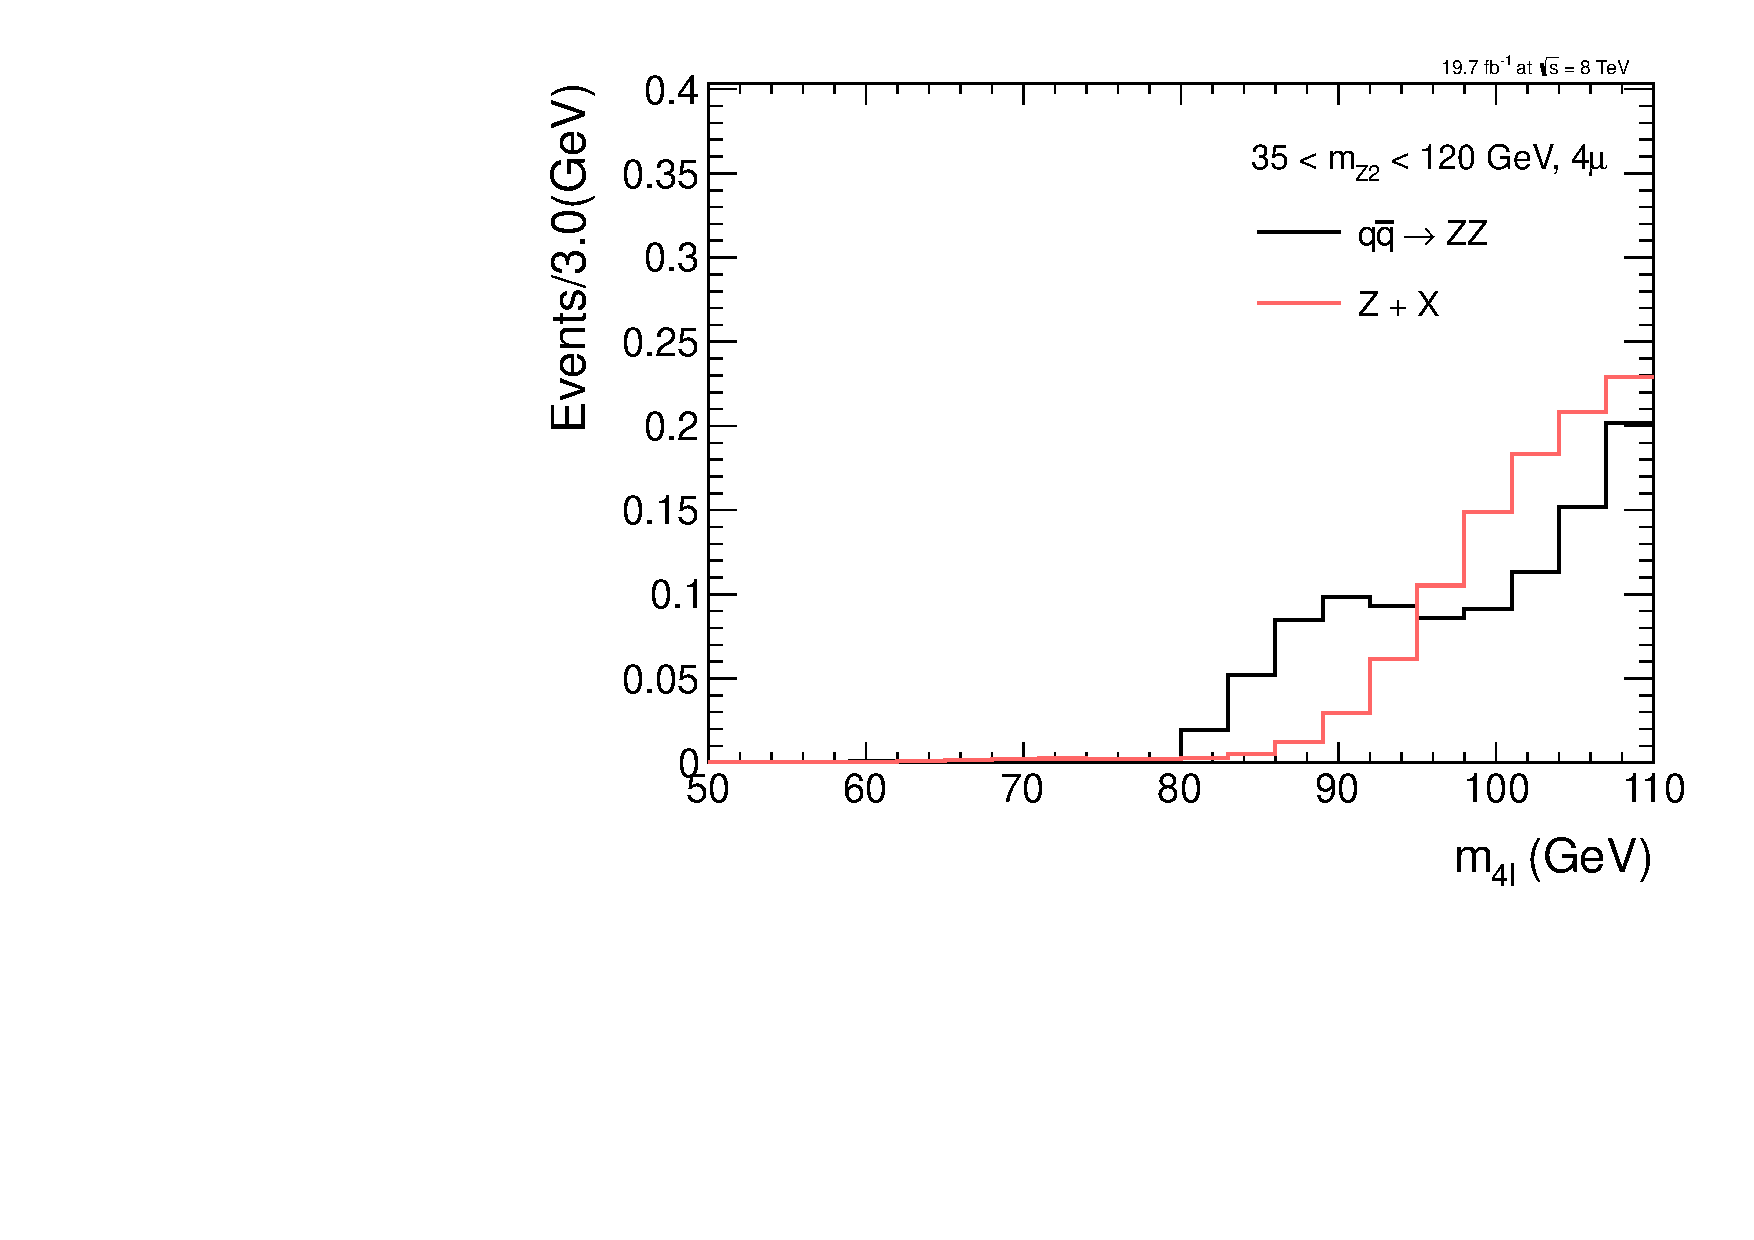
\includegraphics[width=0.32\textwidth,angle=0]{Appendix/figuresZ4l/XSTemplates_4mu_massZ2_35_120_qqZZ_ZJetsCR.pdf}
      \label{fig:z4l_bkg-massZ2-qqZZ-ZX-4mu:d}
    }
    \subfigure[$35.0 \GeV < \mathrm{m}(\mathrm{Z}_{2}) < 120.0 \GeV$]{
      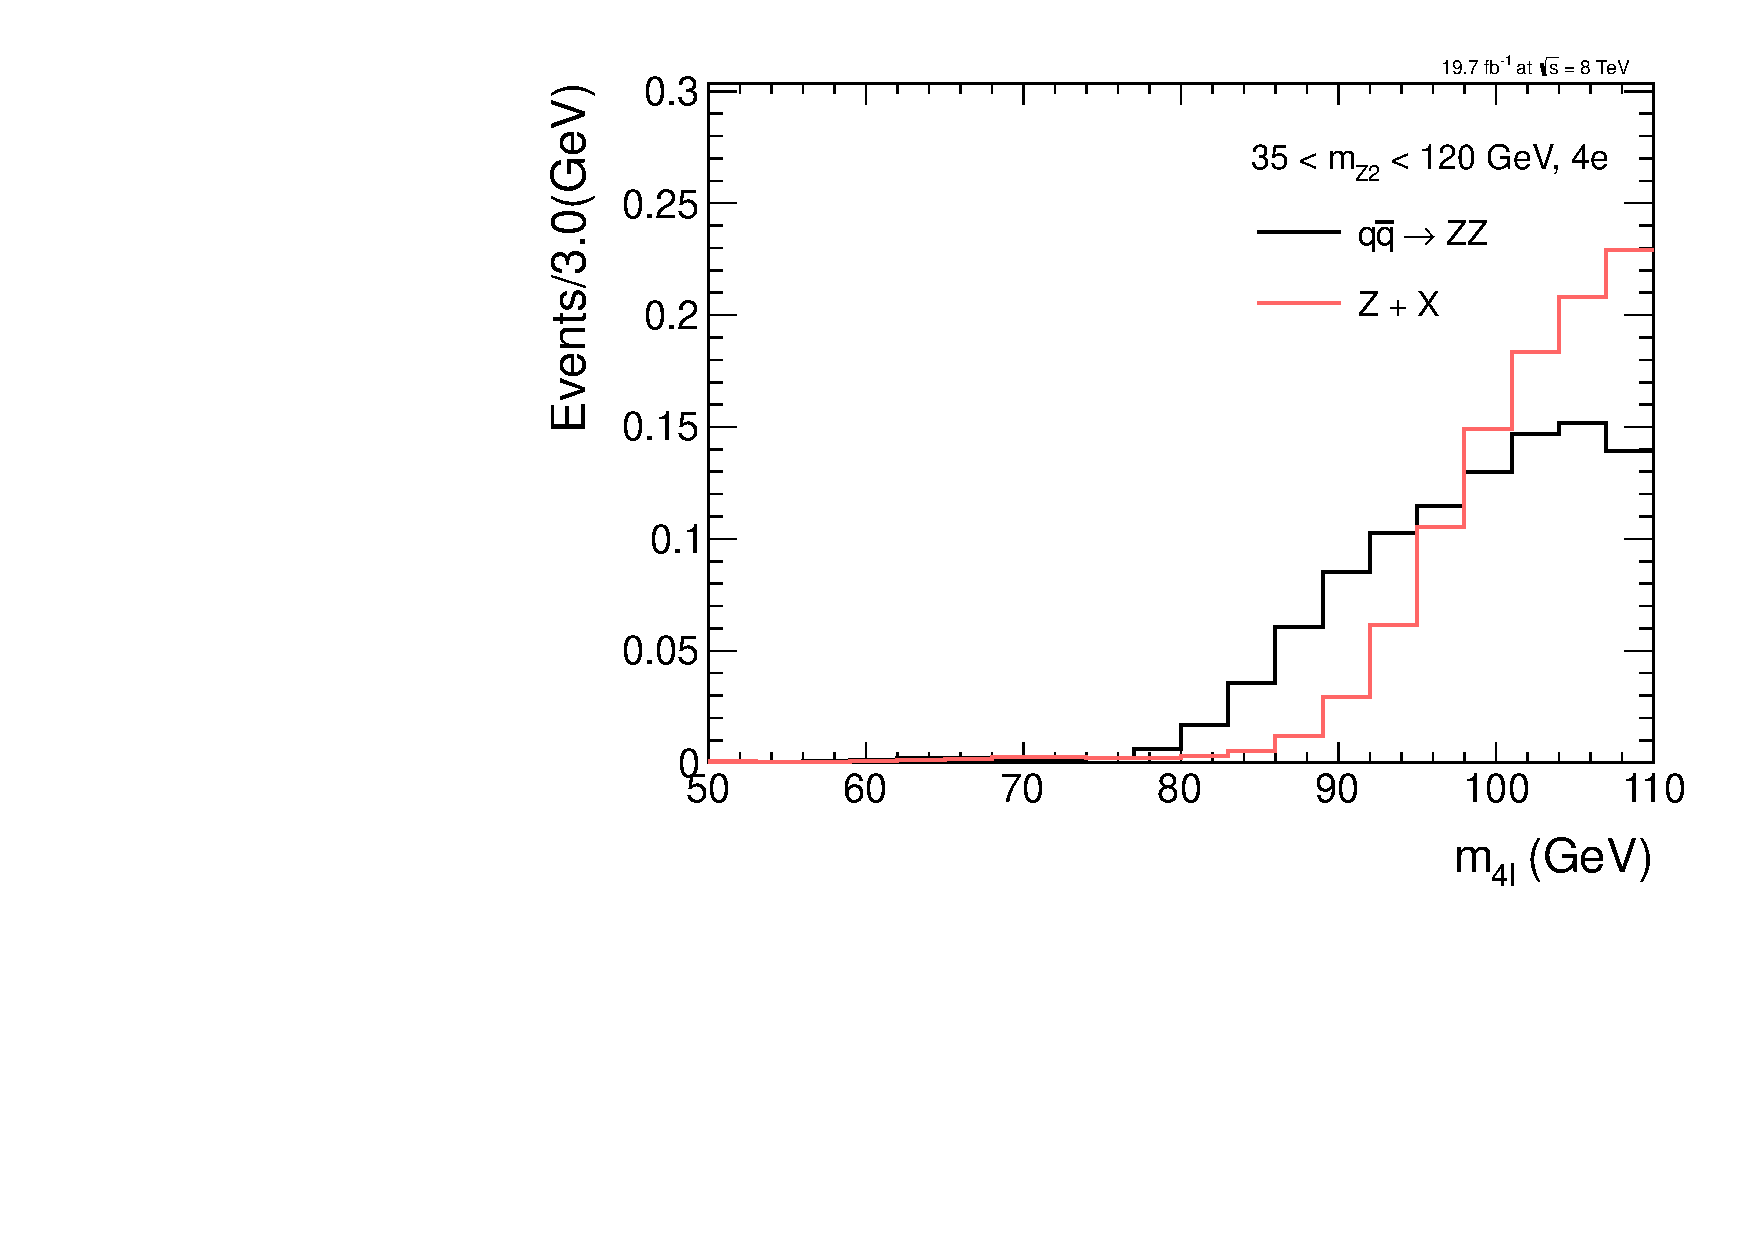
\includegraphics[width=0.32\textwidth,angle=0]{Appendix/figuresZ4l/XSTemplates_4e_massZ2_35_120_qqZZ_ZJetsCR.pdf}
      \label{fig:z4l_bkg-massZ2-qqZZ-ZX-4e:d}
    } \\
    
    \caption{ Distributions of m($4\ell$) for the $qq \rightarrow \mathrm{ZZ}$ and Z+X backgrounds in different bins of $m(\mathrm{Z}_{2})$
for Z$\to$4l measurements 
    for three final states: $2e2\mu$(left), $4\mu$(middle) and $4e$(right).}
  \label{fig:z4l_bkg-massZ2-qqZZ-ZX}
  
 \end{center}
\end{figure} 

 \clearpage
 
 \begin{figure}[!ht]
  \begin{center}
  
    \subfigure[$12.0 \GeV < \mathrm{m}(\mathrm{Z}_{2}) < 20.0 \GeV$]{
      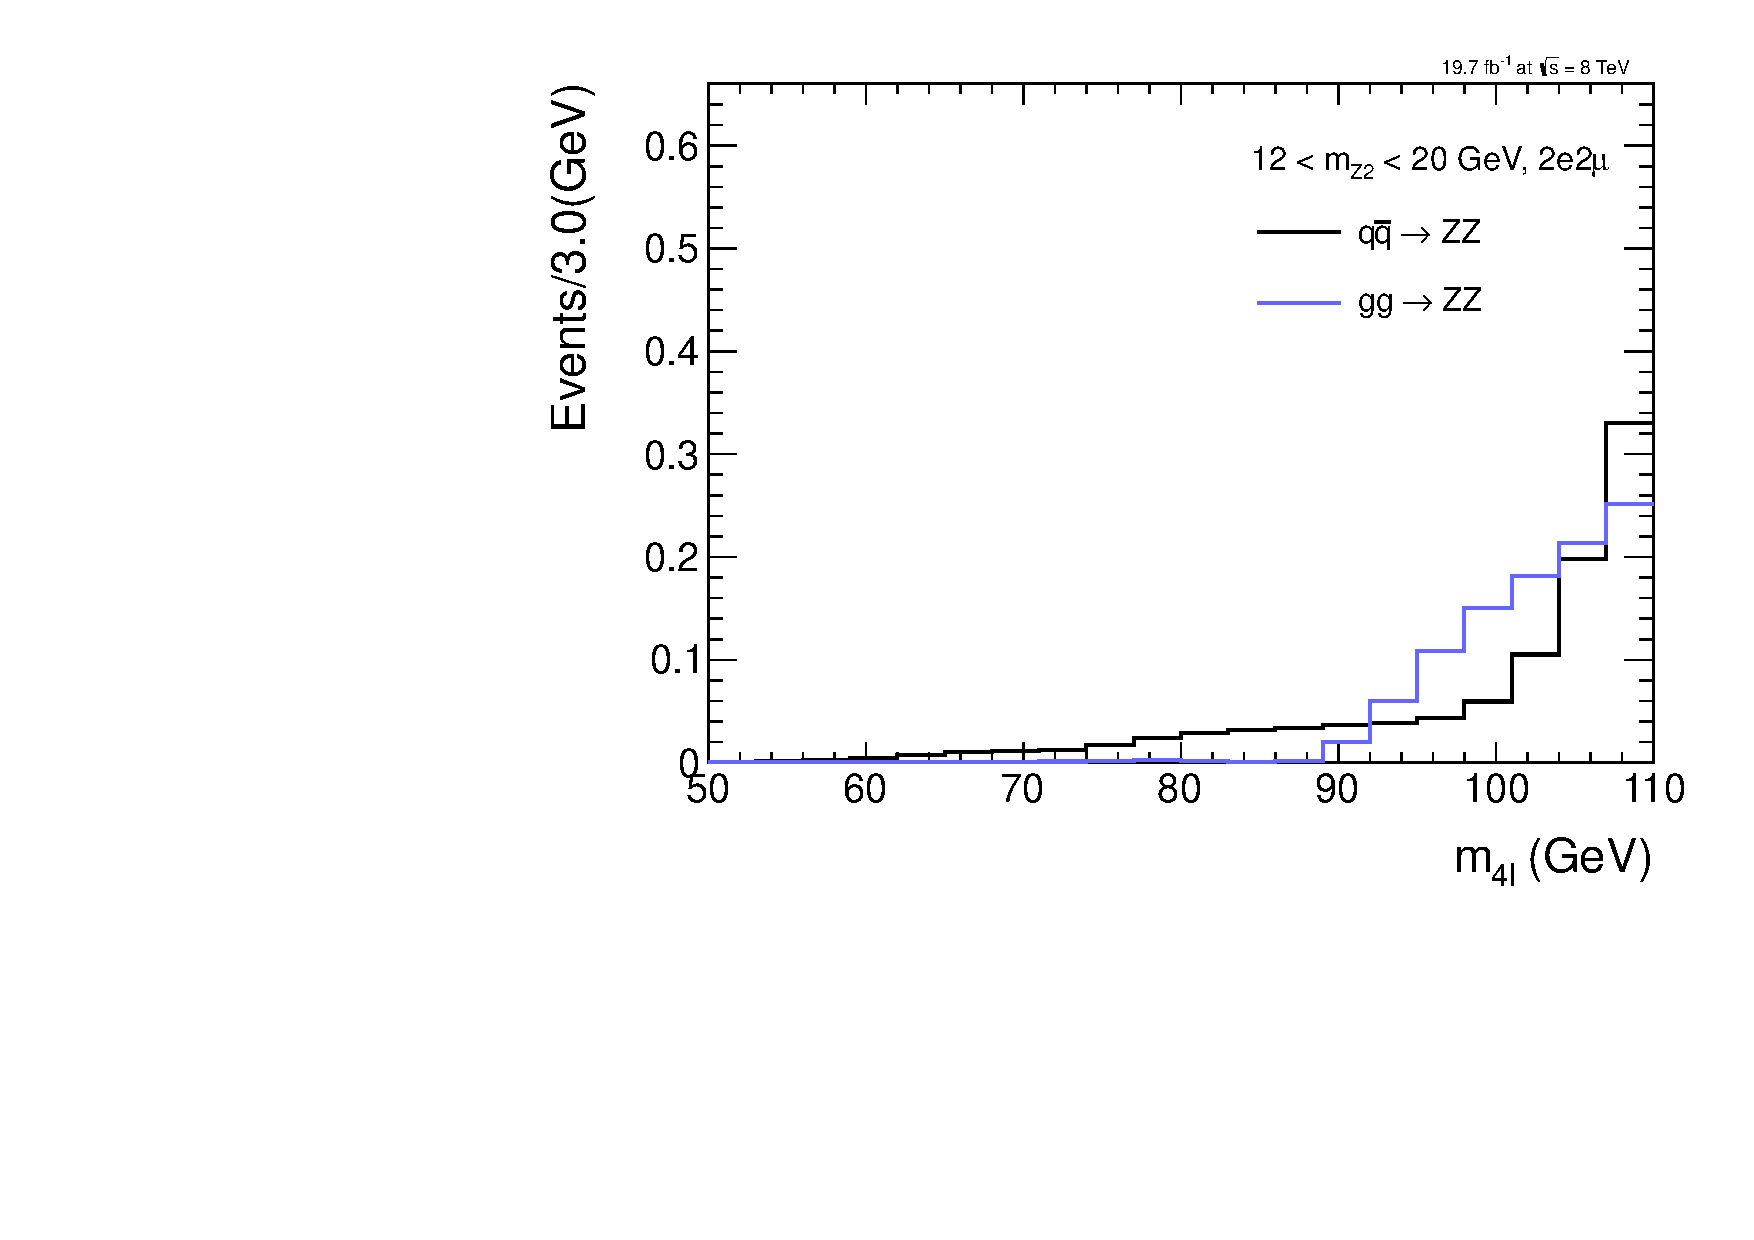
\includegraphics[width=0.32\textwidth,angle=0]{Appendix/figuresZ4l/XSTemplates_2e2mu_massZ2_12_20_qqZZ_ggZZ.pdf}
      \label{fig:z4l_bkg-massZ2-qqZZ-ggZZ-2e2mu:a}
    }    
    \subfigure[$12.0 \GeV < \mathrm{m}(\mathrm{Z}_{2}) < 20.0 \GeV$]{
      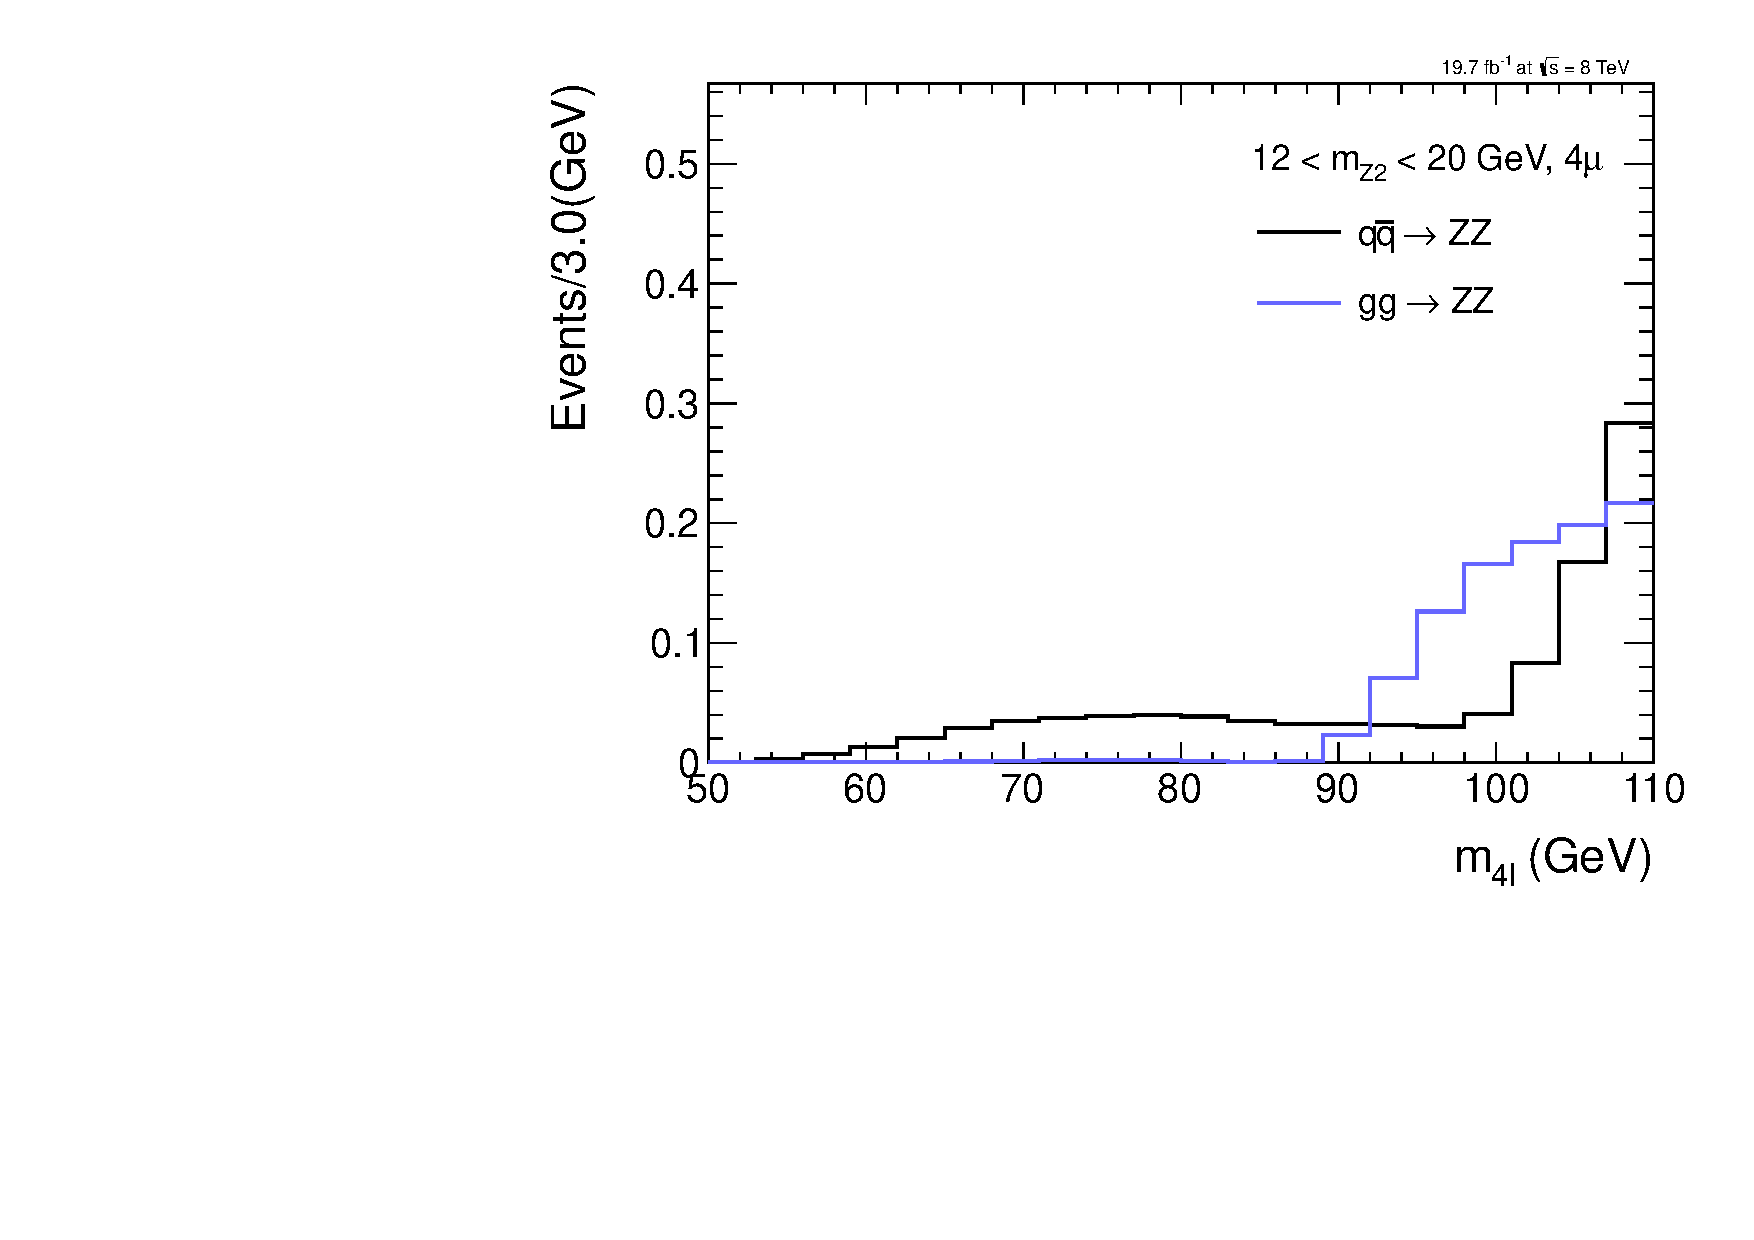
\includegraphics[width=0.32\textwidth,angle=0]{Appendix/figuresZ4l/XSTemplates_4mu_massZ2_12_20_qqZZ_ggZZ.pdf}
      \label{fig:z4l_bkg-massZ2-qqZZ-ggZZ-4mu:a}
    }    
    \subfigure[$12.0 \GeV < \mathrm{m}(\mathrm{Z}_{2}) < 20.0 \GeV$]{
      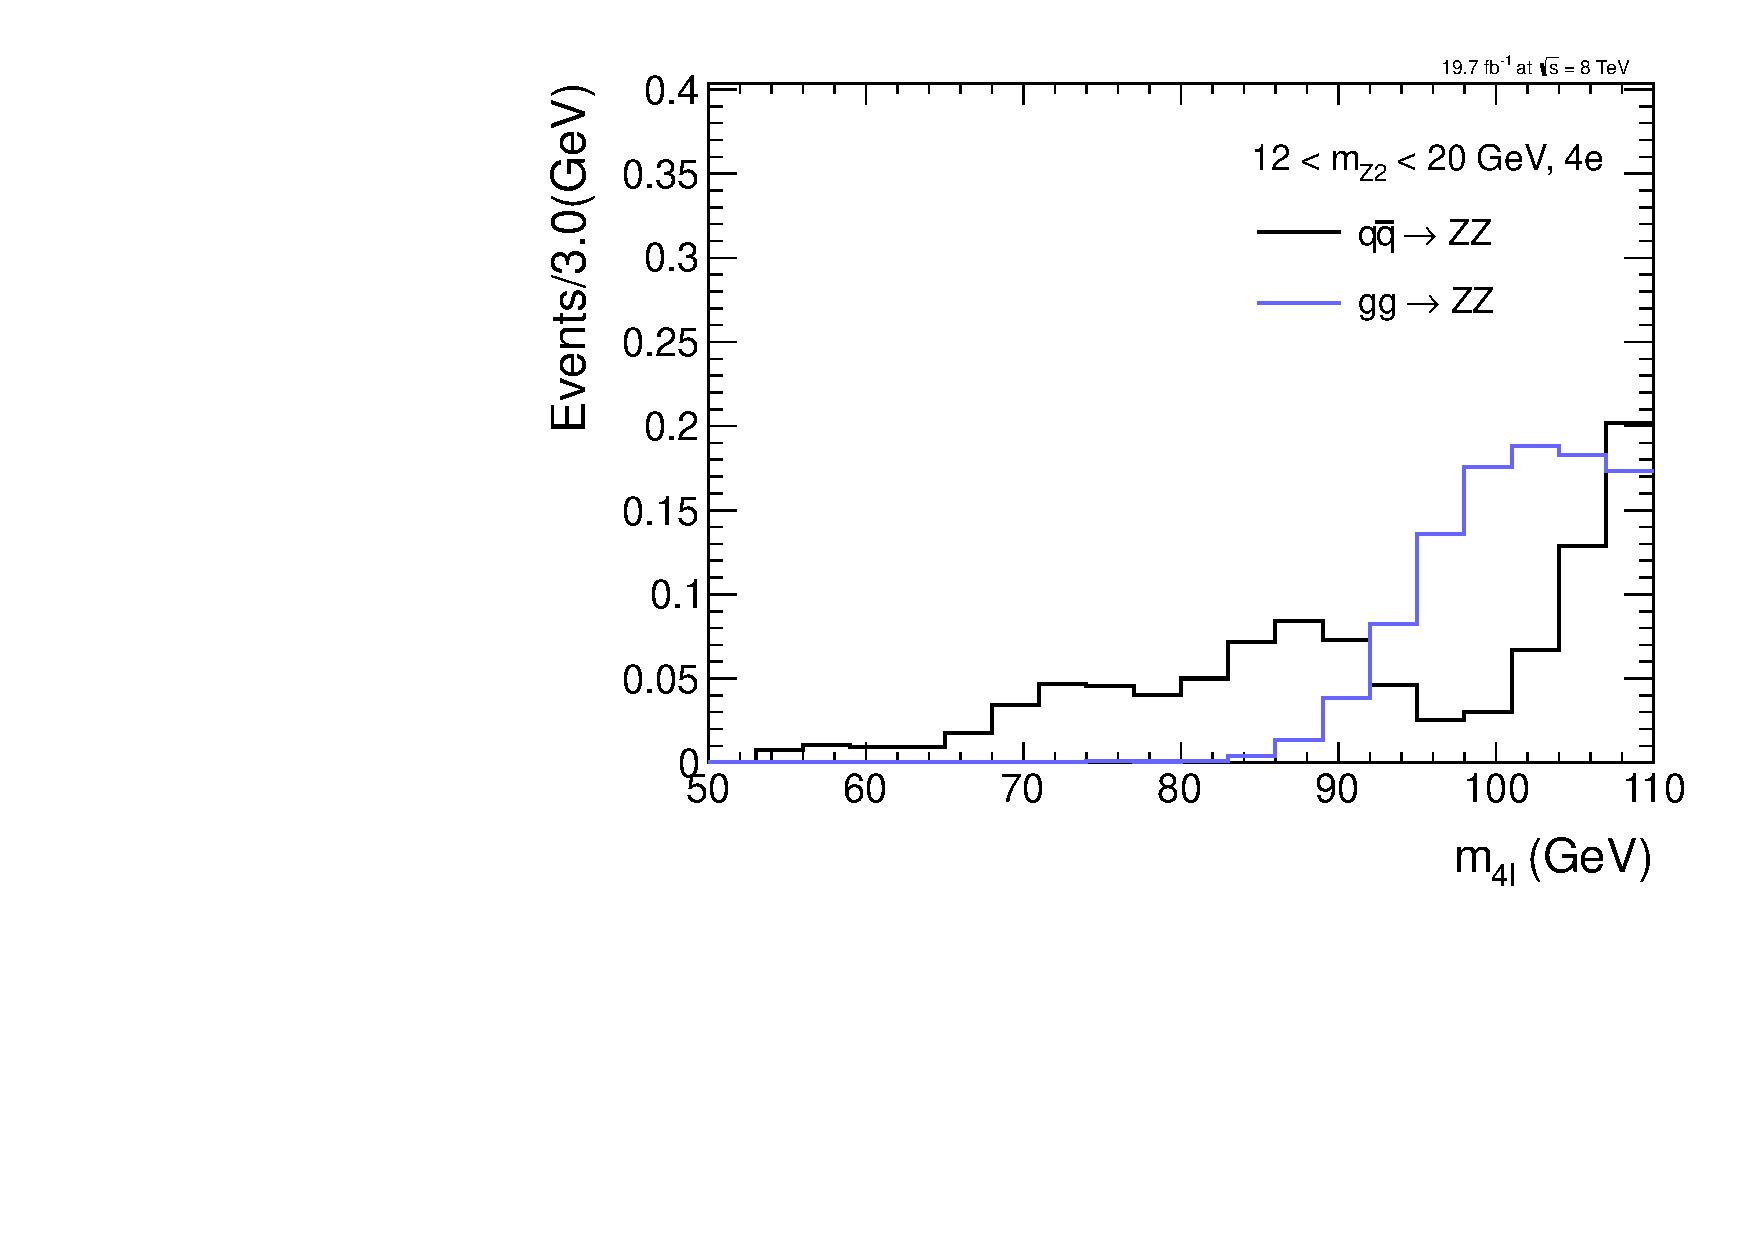
\includegraphics[width=0.32\textwidth,angle=0]{Appendix/figuresZ4l/XSTemplates_4e_massZ2_12_20_qqZZ_ggZZ.pdf}
      \label{fig:z4l_bkg-massZ2-qqZZ-ggZZ-4e:a}
    }    \\

    \subfigure[$20.0 \GeV < \mathrm{m}(\mathrm{Z}_{2}) < 28.0 \GeV$]{
      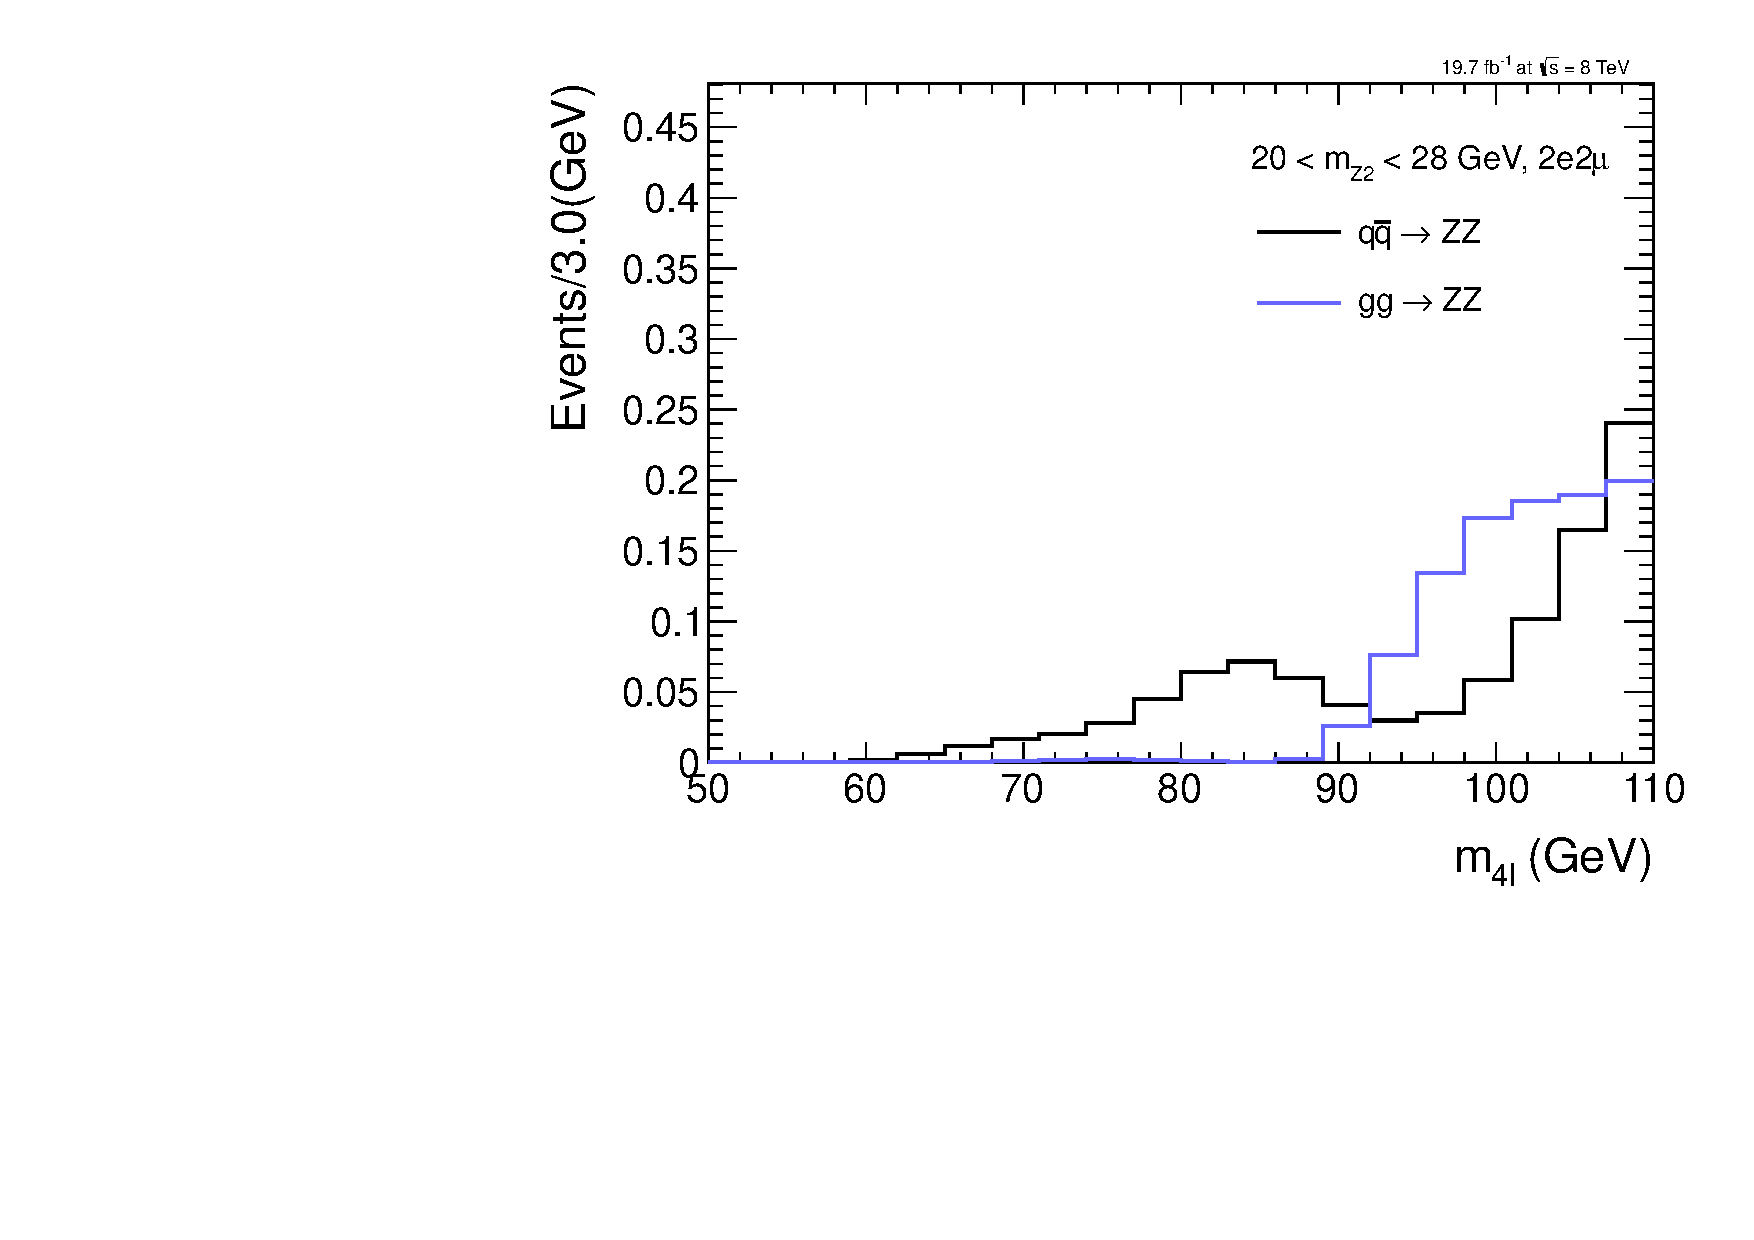
\includegraphics[width=0.32\textwidth,angle=0]{Appendix/figuresZ4l/XSTemplates_2e2mu_massZ2_20_28_qqZZ_ggZZ.pdf}
      \label{fig:z4l_bkg-massZ2-qqZZ-ggZZ-2e2mu:b}
    }
    \subfigure[$20.0 \GeV < \mathrm{m}(\mathrm{Z}_{2}) < 28.0 \GeV$]{
      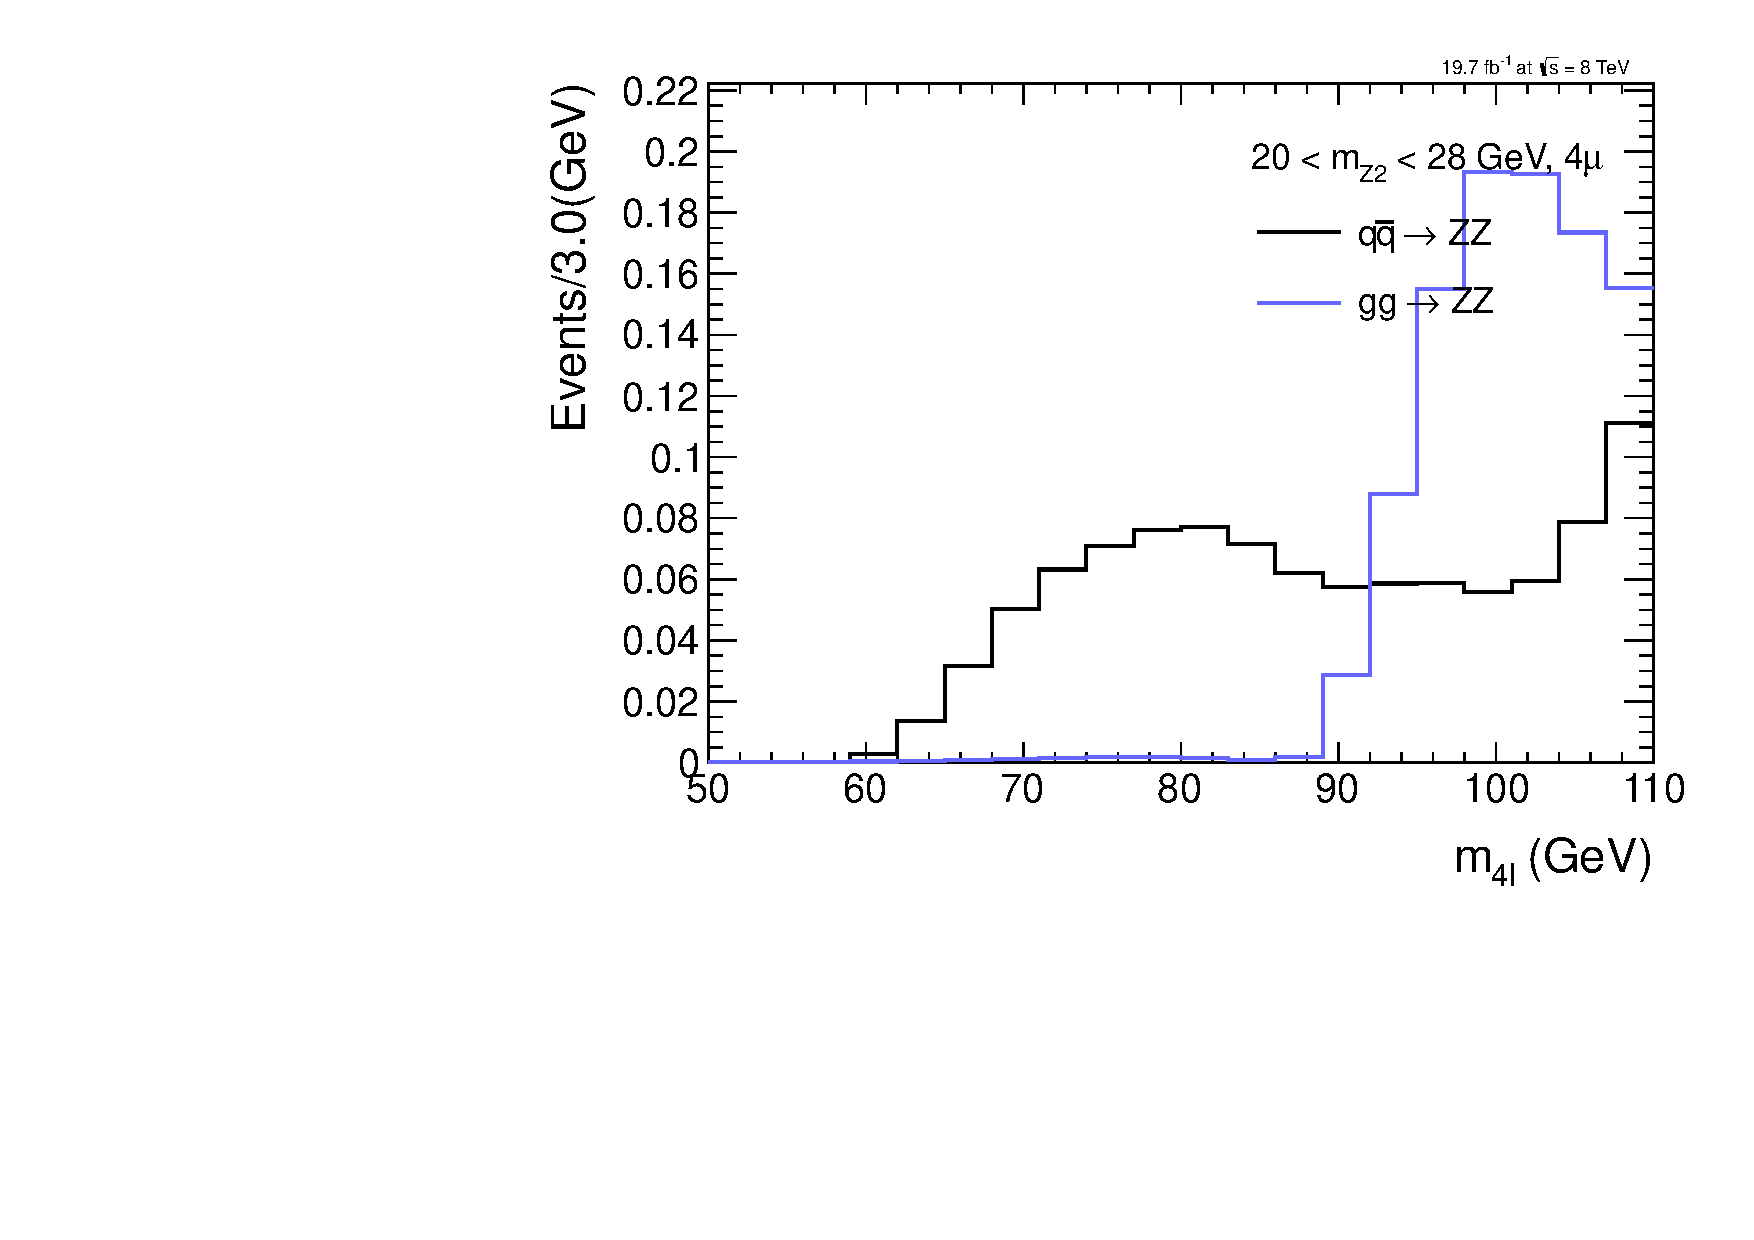
\includegraphics[width=0.32\textwidth,angle=0]{Appendix/figuresZ4l/XSTemplates_4mu_massZ2_20_28_qqZZ_ggZZ.pdf}
      \label{fig:z4l_bkg-massZ2-qqZZ-ggZZ-4mu:b}
    } 
    \subfigure[$20.0 \GeV < \mathrm{m}(\mathrm{Z}_{2}) < 28.0 \GeV$]{
      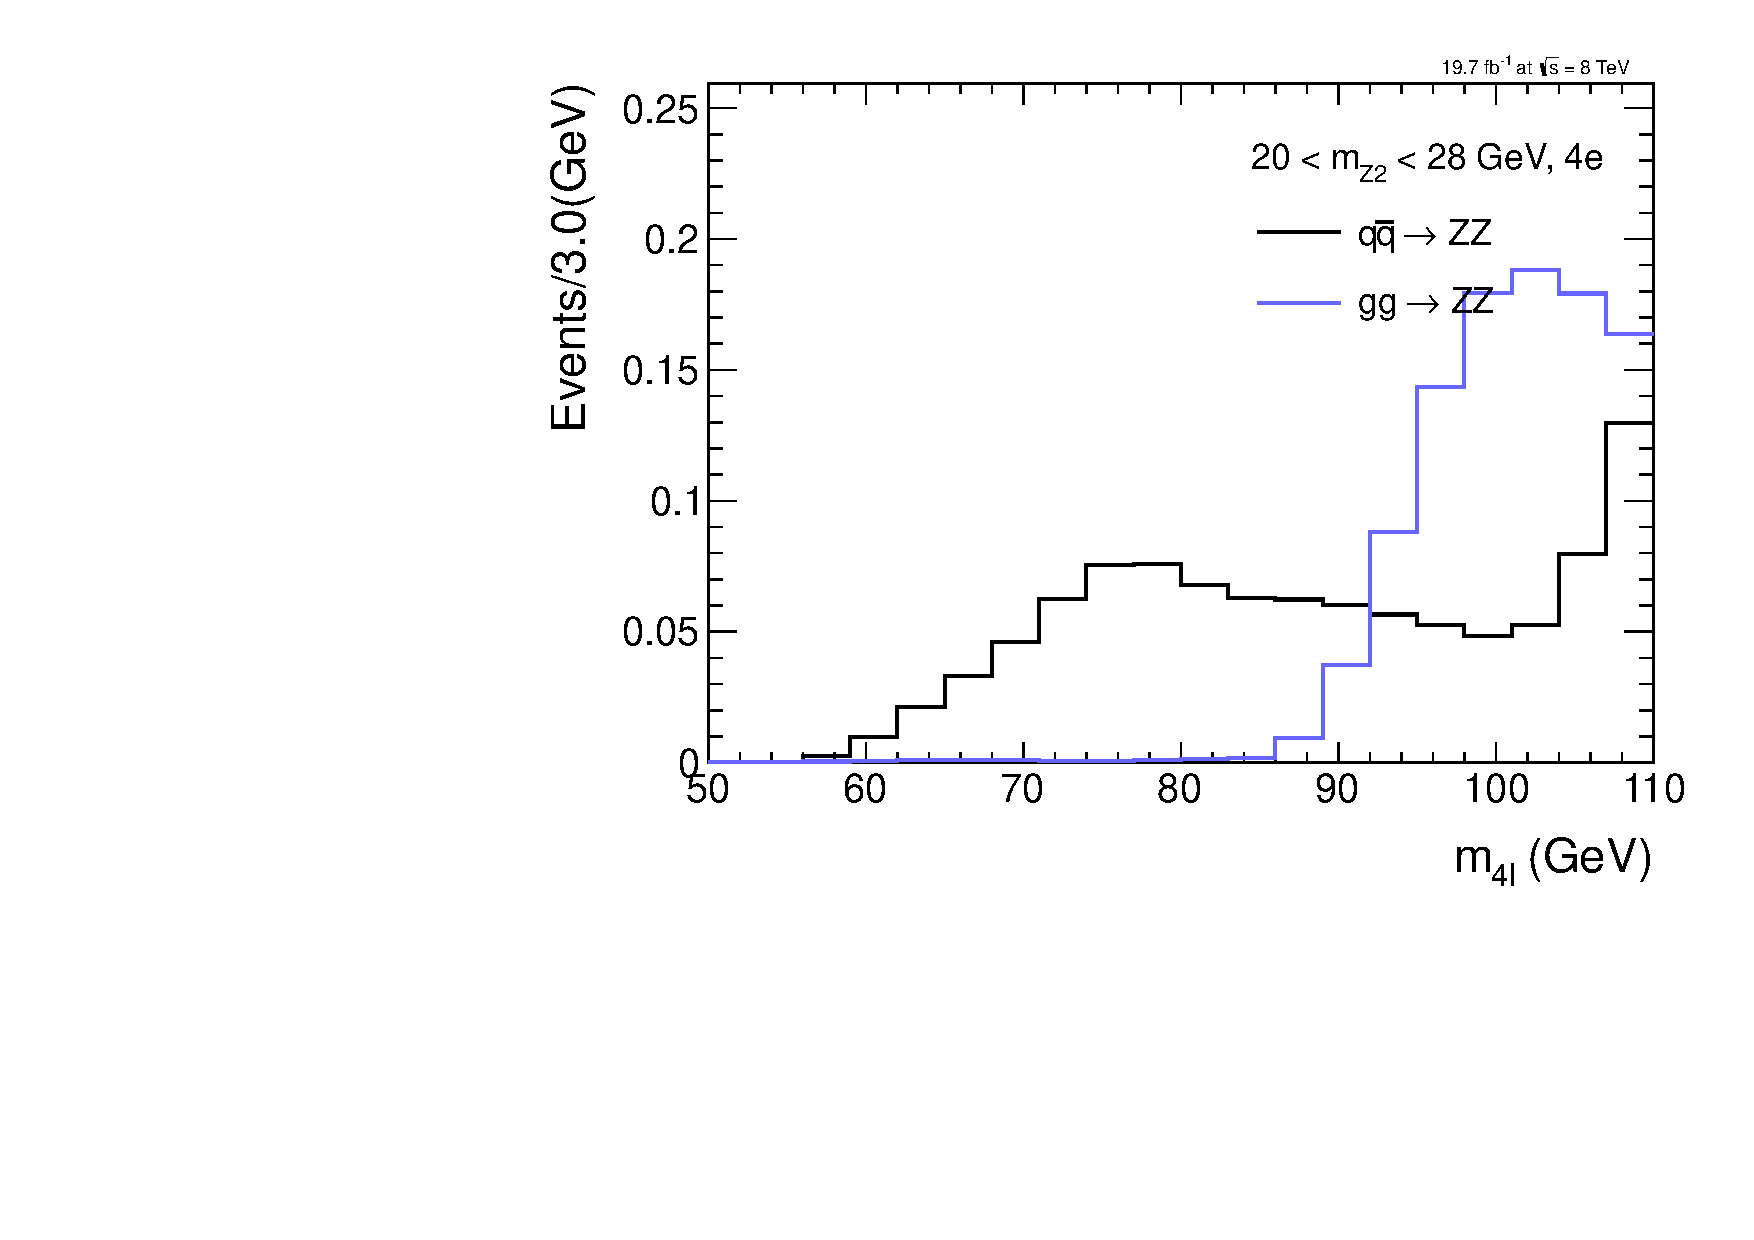
\includegraphics[width=0.32\textwidth,angle=0]{Appendix/figuresZ4l/XSTemplates_4e_massZ2_20_28_qqZZ_ggZZ.pdf}
      \label{fig:z4l_bkg-massZ2-qqZZ-ggZZ-4e:b}
    } \\
    
    \subfigure[$28.0 \GeV < \mathrm{m}(\mathrm{Z}_{2}) < 35.0 \GeV$]{
      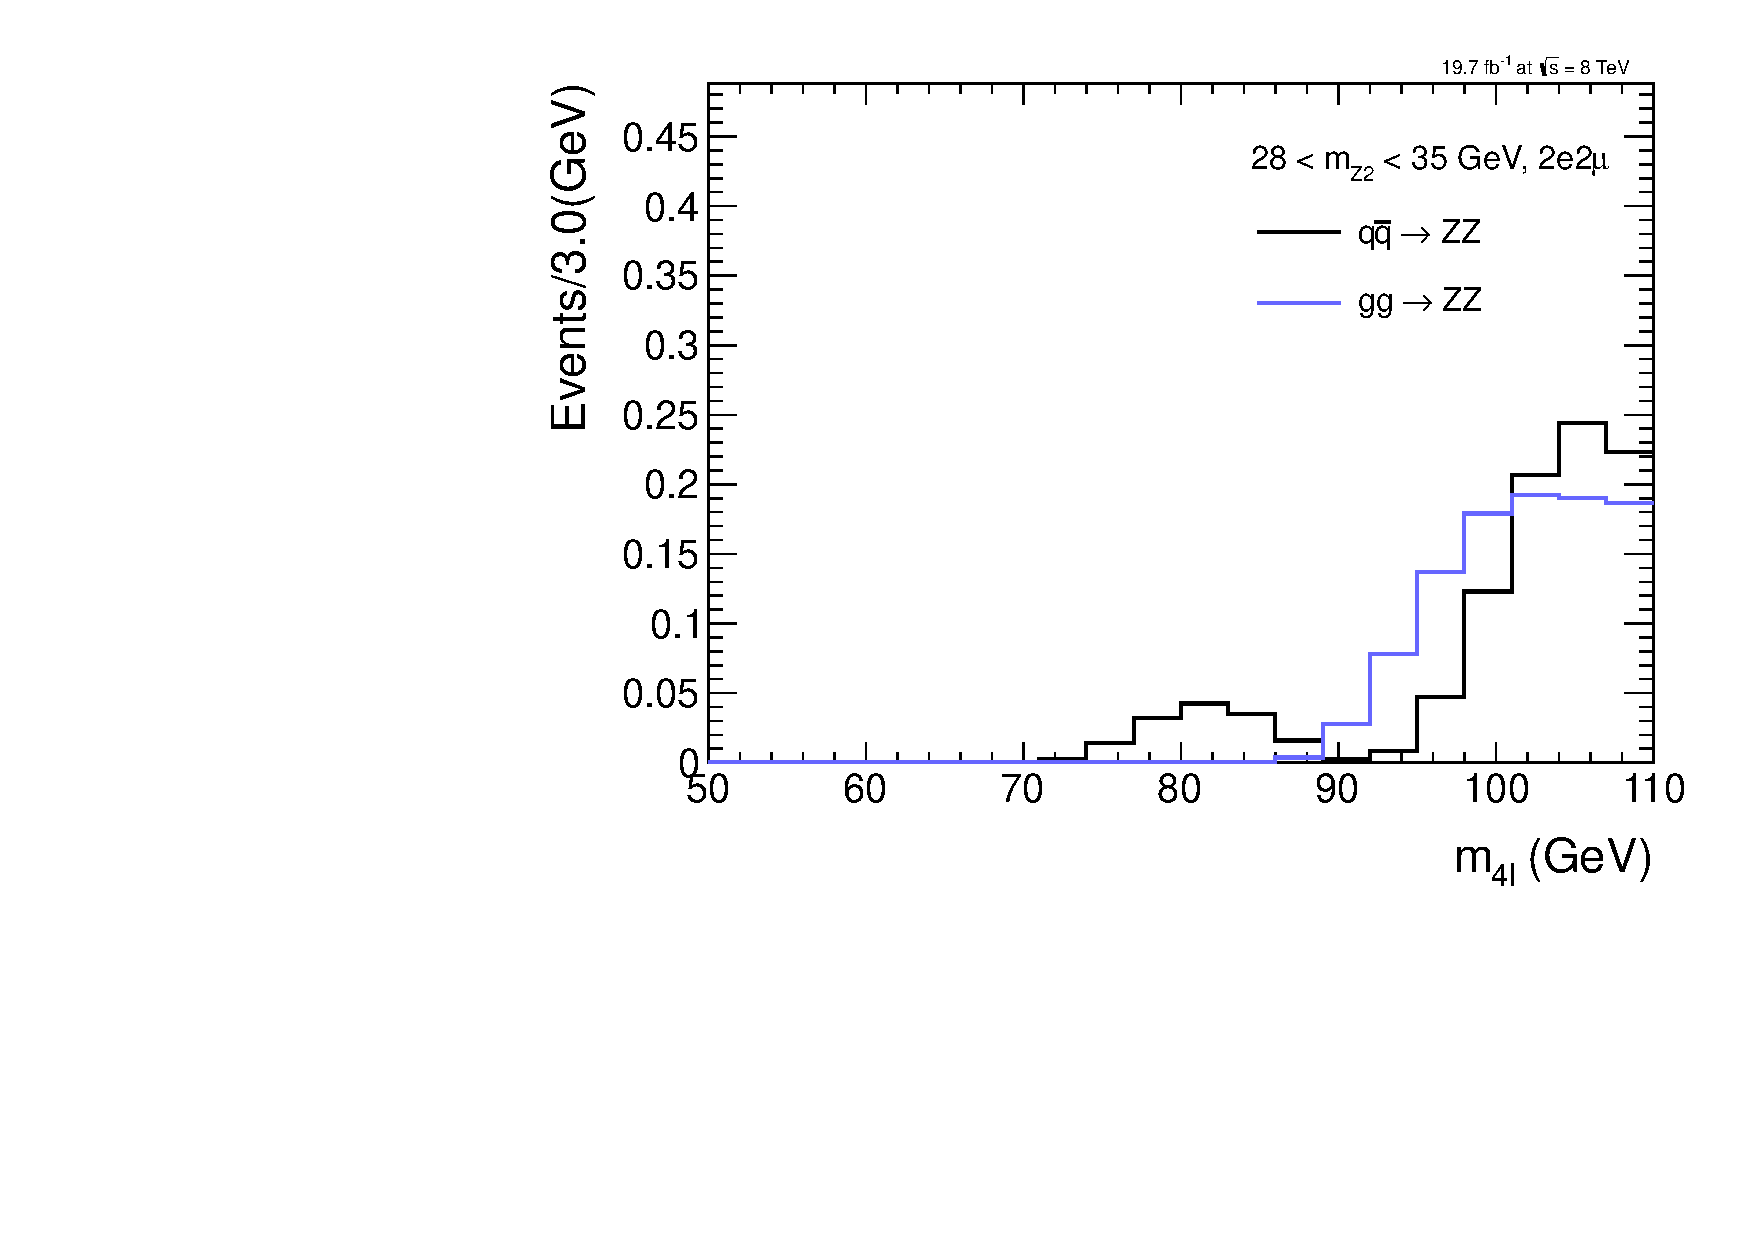
\includegraphics[width=0.32\textwidth,angle=0]{Appendix/figuresZ4l/XSTemplates_2e2mu_massZ2_28_35_qqZZ_ggZZ.pdf}
      \label{fig:z4l_bkg-massZ2-qqZZ-ggZZ-2e2mu:c}
    }
    \subfigure[$28.0 \GeV < \mathrm{m}(\mathrm{Z}_{2}) < 35.0 \GeV$]{
      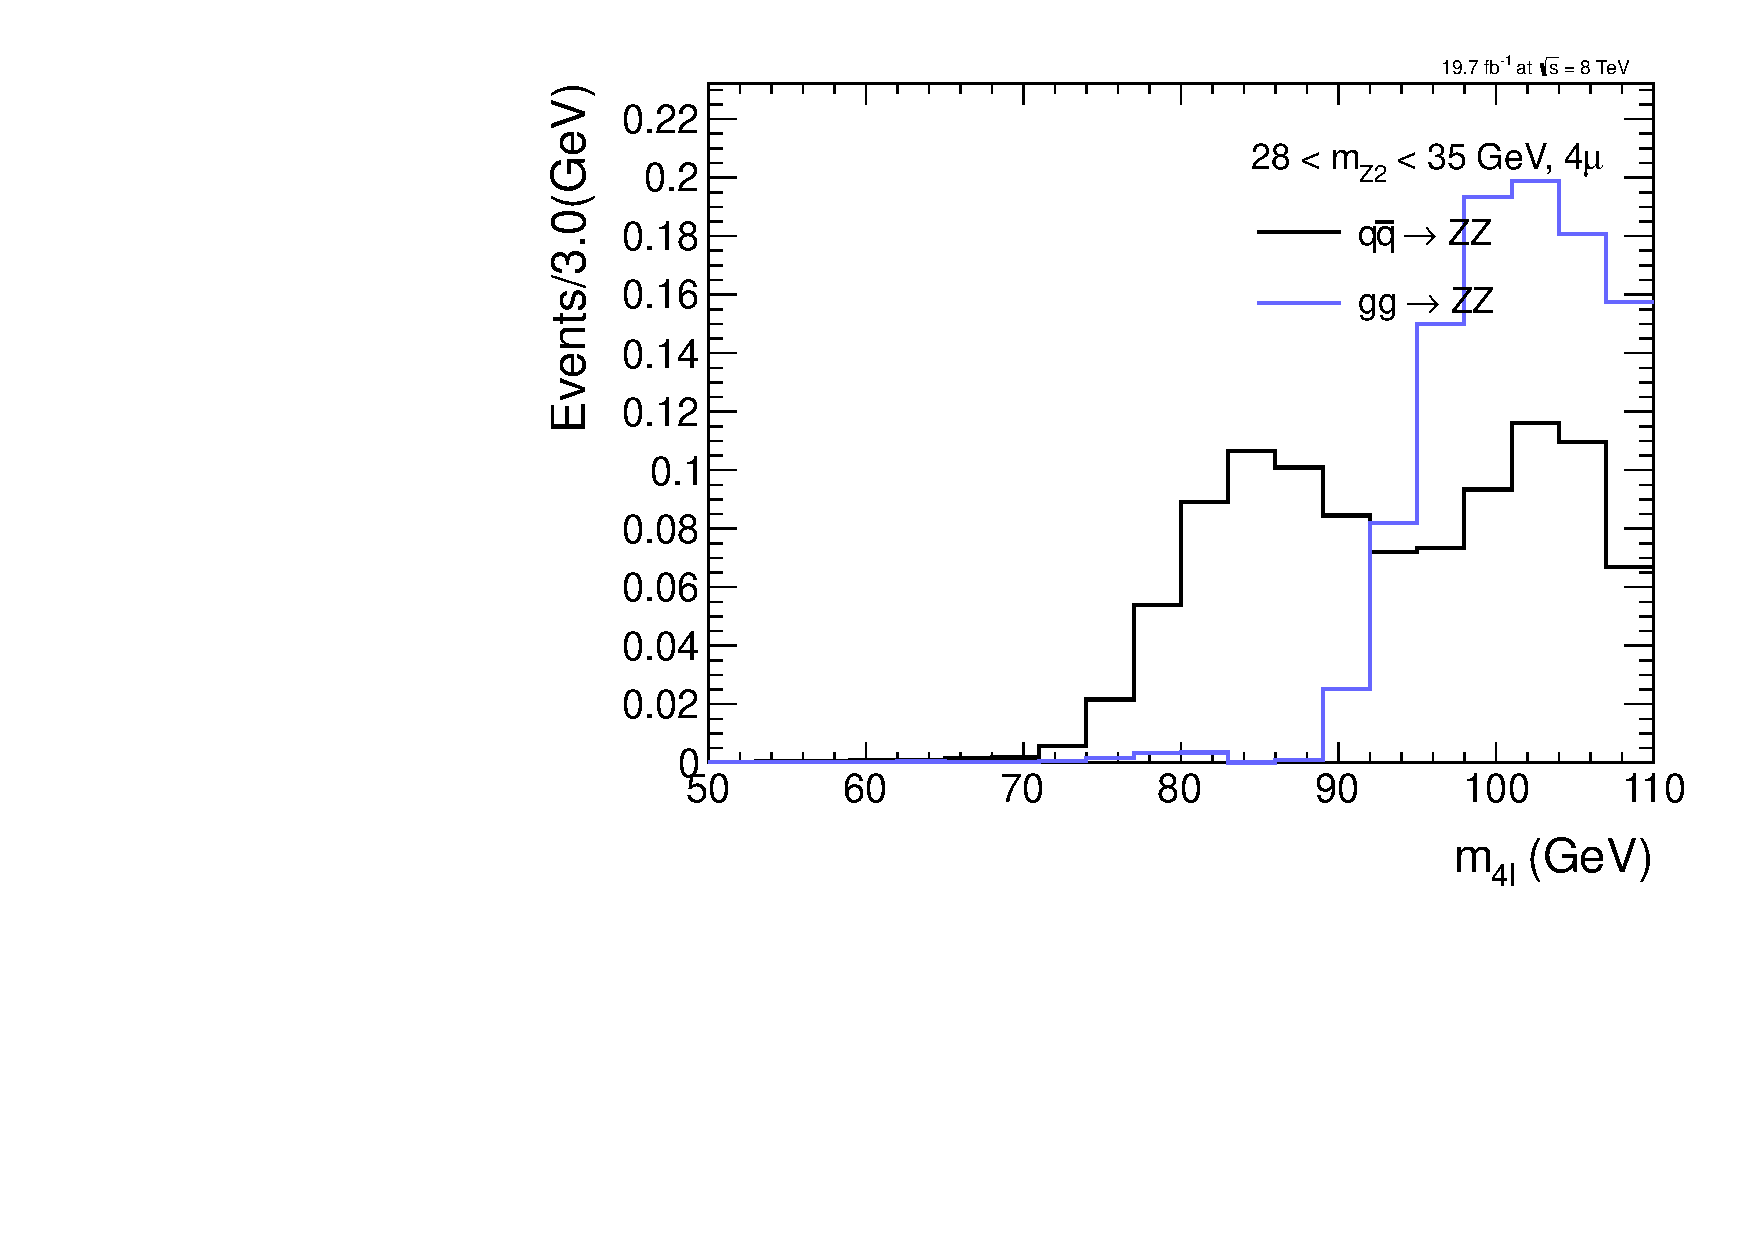
\includegraphics[width=0.32\textwidth,angle=0]{Appendix/figuresZ4l/XSTemplates_4mu_massZ2_28_35_qqZZ_ggZZ.pdf}
      \label{fig:z4l_bkg-massZ2-qqZZ-ggZZ-4mu:c}
    }
    \subfigure[$28.0 \GeV < \mathrm{m}(\mathrm{Z}_{2}) < 35.0 \GeV$]{
      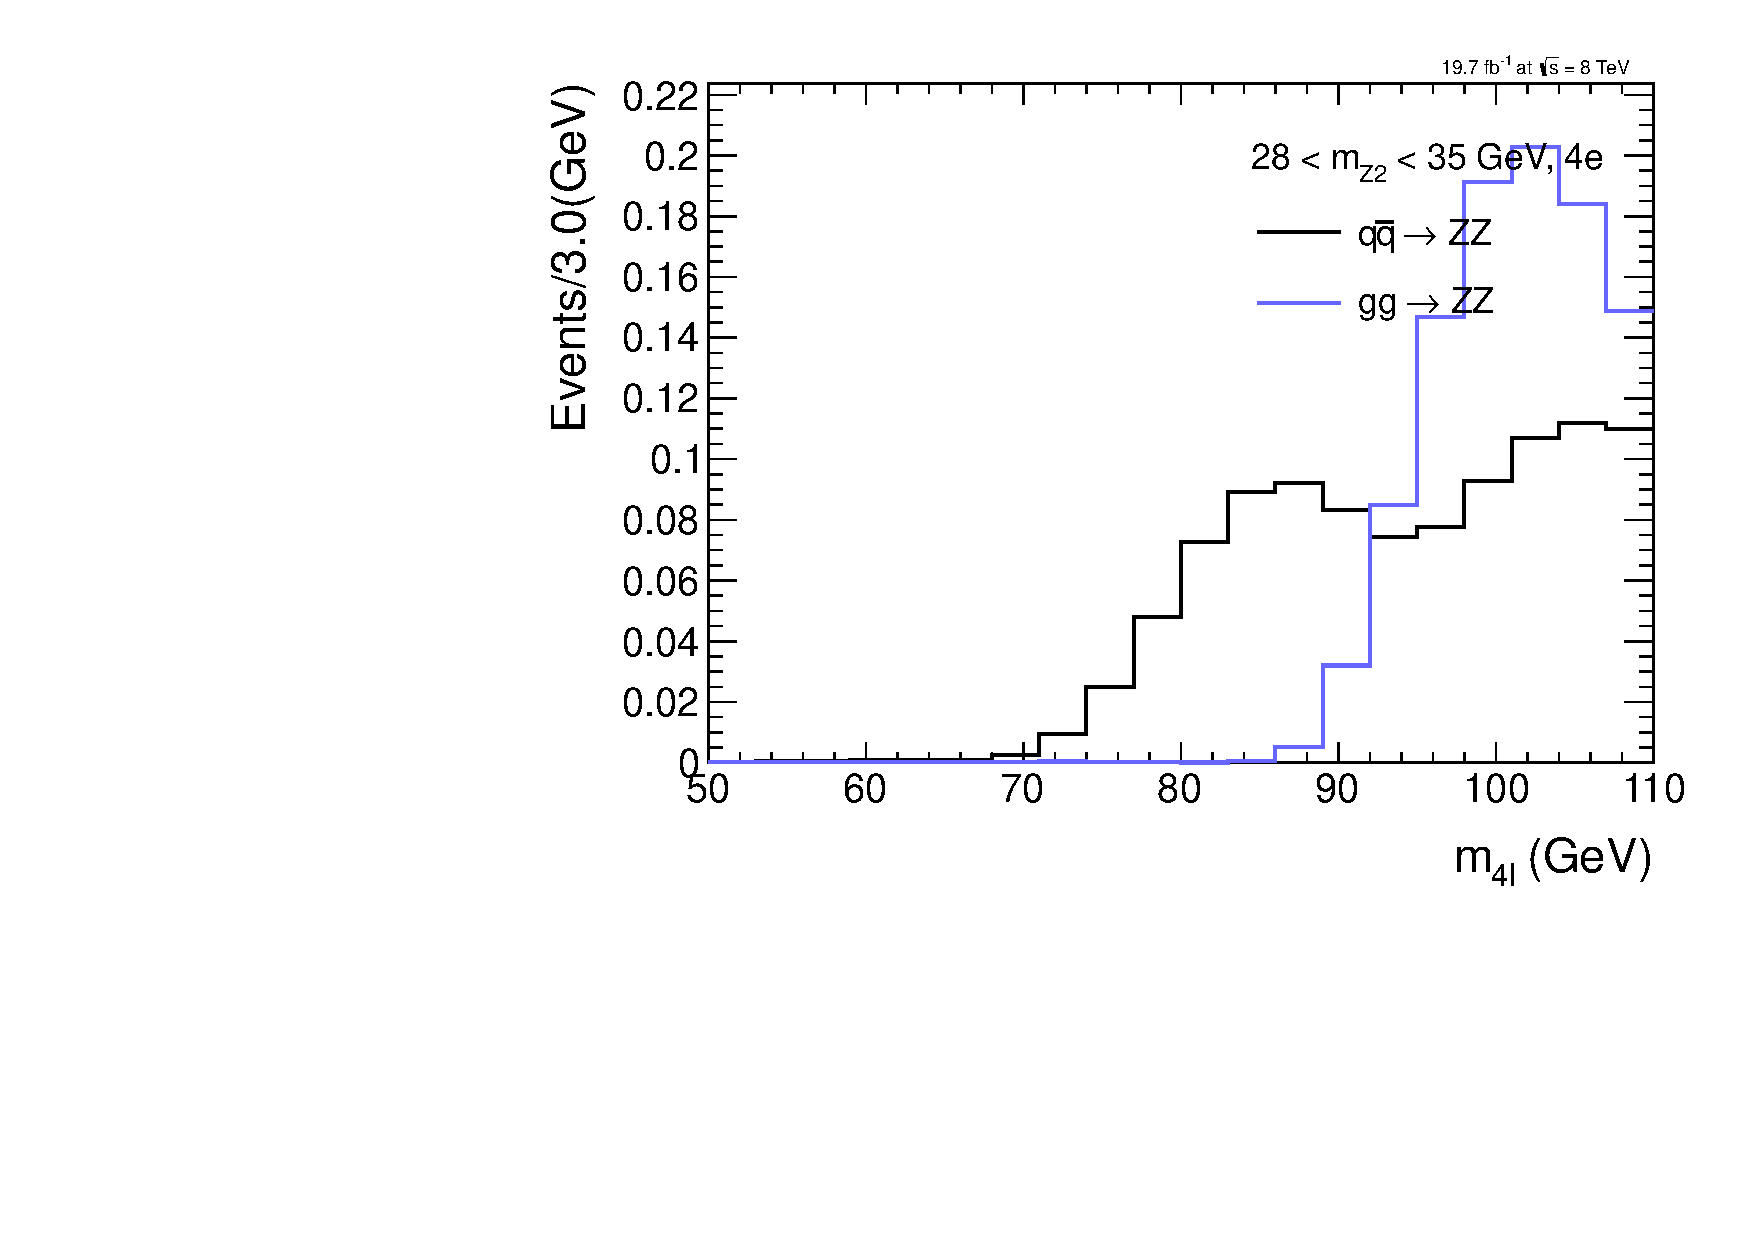
\includegraphics[width=0.32\textwidth,angle=0]{Appendix/figuresZ4l/XSTemplates_4e_massZ2_28_35_qqZZ_ggZZ.pdf}
      \label{fig:z4l_bkg-massZ2-qqZZ-ggZZ-4e:c}
    } \\
    
    \subfigure[$35.0 \GeV < \mathrm{m}(\mathrm{Z}_{2}) < 120.0 \GeV$]{
      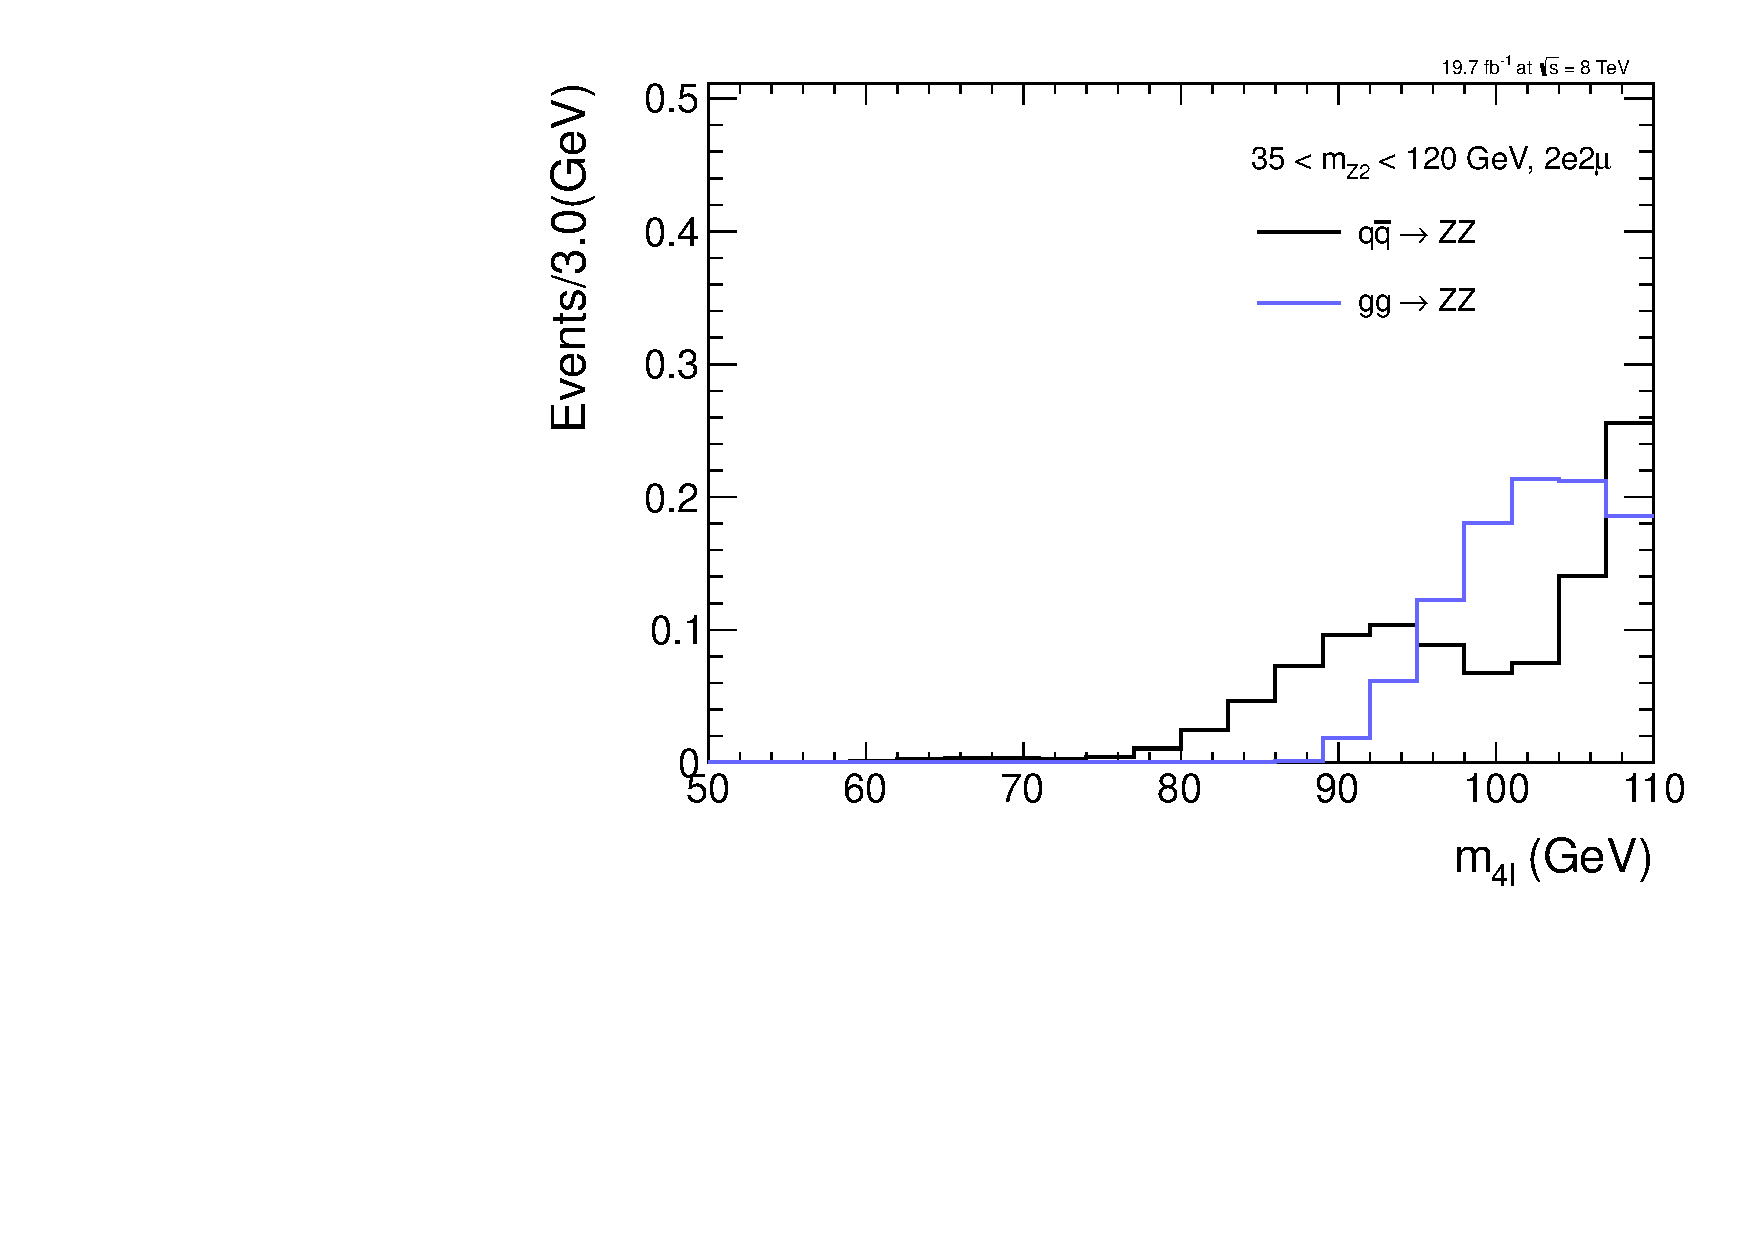
\includegraphics[width=0.32\textwidth,angle=0]{Appendix/figuresZ4l/XSTemplates_2e2mu_massZ2_35_120_qqZZ_ggZZ.pdf}
      \label{fig:z4l_bkg-massZ2-qqZZ-ggZZ-2e2mu:d}
    }
    \subfigure[$35.0 \GeV < \mathrm{m}(\mathrm{Z}_{2}) < 120.0 \GeV$]{
      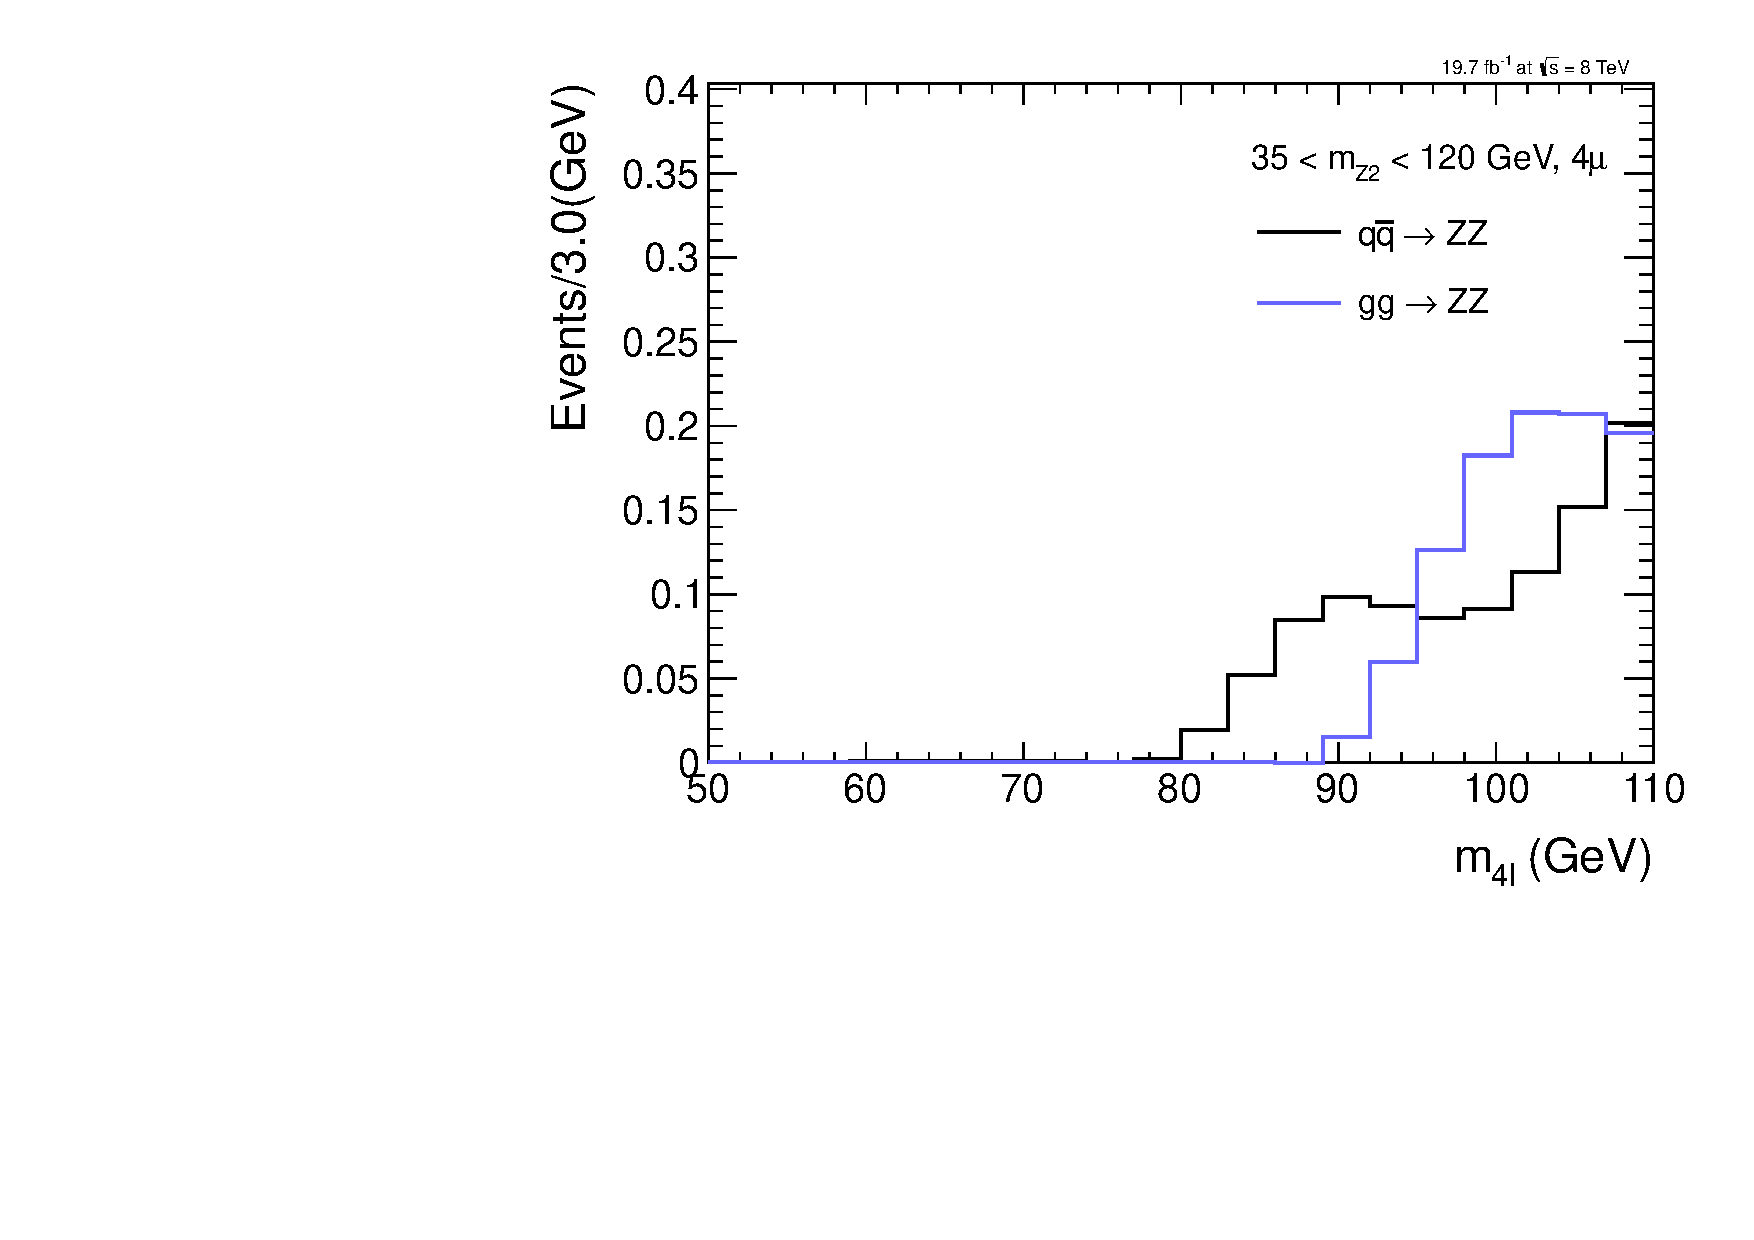
\includegraphics[width=0.32\textwidth,angle=0]{Appendix/figuresZ4l/XSTemplates_4mu_massZ2_35_120_qqZZ_ggZZ.pdf}
      \label{fig:z4l_bkg-massZ2-qqZZ-ggZZ-4mu:d}
    }
    \subfigure[$35.0 \GeV < \mathrm{m}(\mathrm{Z}_{2}) < 120.0 \GeV$]{
      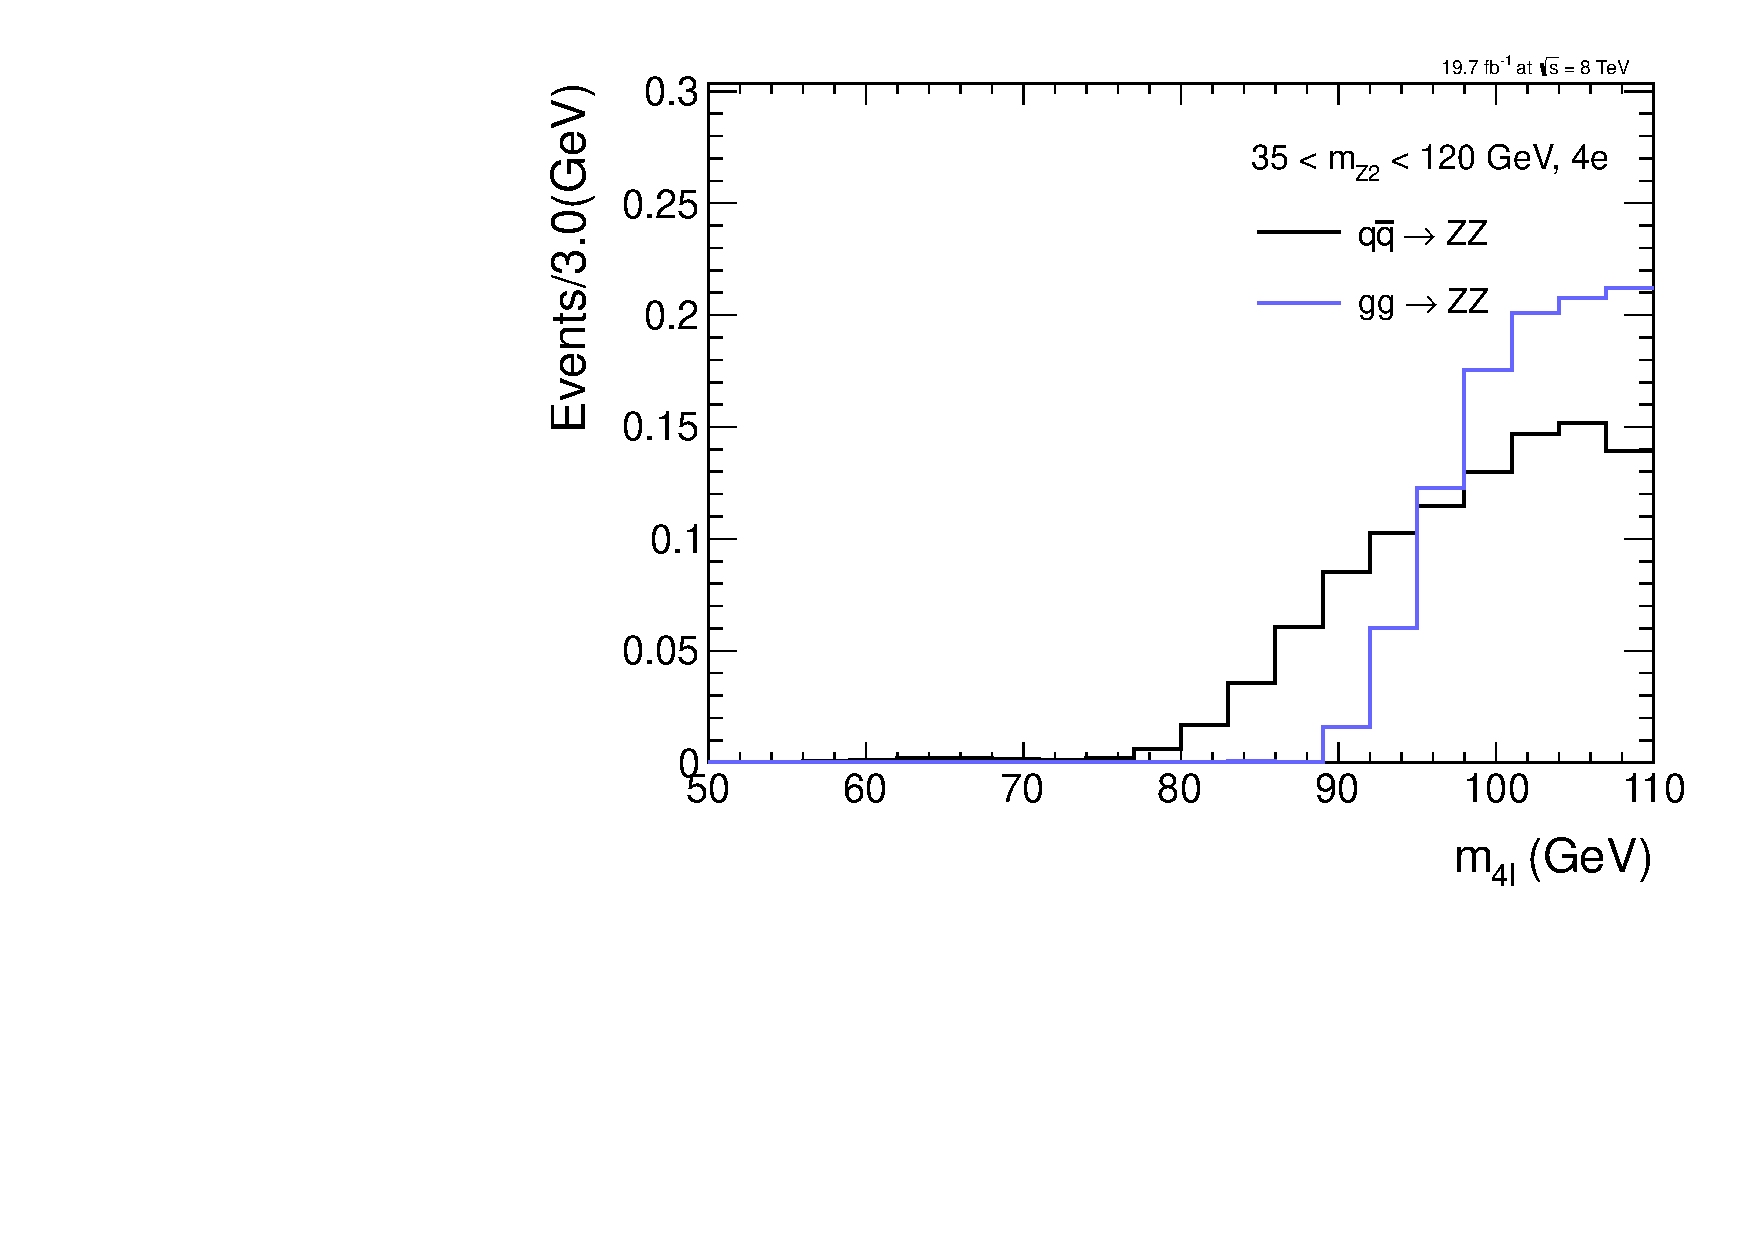
\includegraphics[width=0.32\textwidth,angle=0]{Appendix/figuresZ4l/XSTemplates_4e_massZ2_35_120_qqZZ_ggZZ.pdf}
      \label{fig:z4l_bkg-massZ2-qqZZ-ggZZ-4e:d}
    } \\
    
    \caption{ Distributions of m($4\ell$) for the $qq \rightarrow \mathrm{ZZ}$ and $gg \rightarrow \mathrm{ZZ}$ backgrounds 
    in different bins of $m(\mathrm{Z}_{2})$
for Z$\to$4l measurements
 for three final states: $2e2\mu$(left), $4\mu$(middle) and $4e$(right).}
  \label{fig:z4l_bkg-massZ2-qqZZ-ggZZ}
  
 \end{center}
\end{figure} 

\clearpage

\subsection{Background shapes in bins of $|y(4\ell)|$ }

\begin{figure}[!ht]
  \begin{center}
  
    \subfigure[$0.0 < |y(4\ell)| < 0.4$]{
      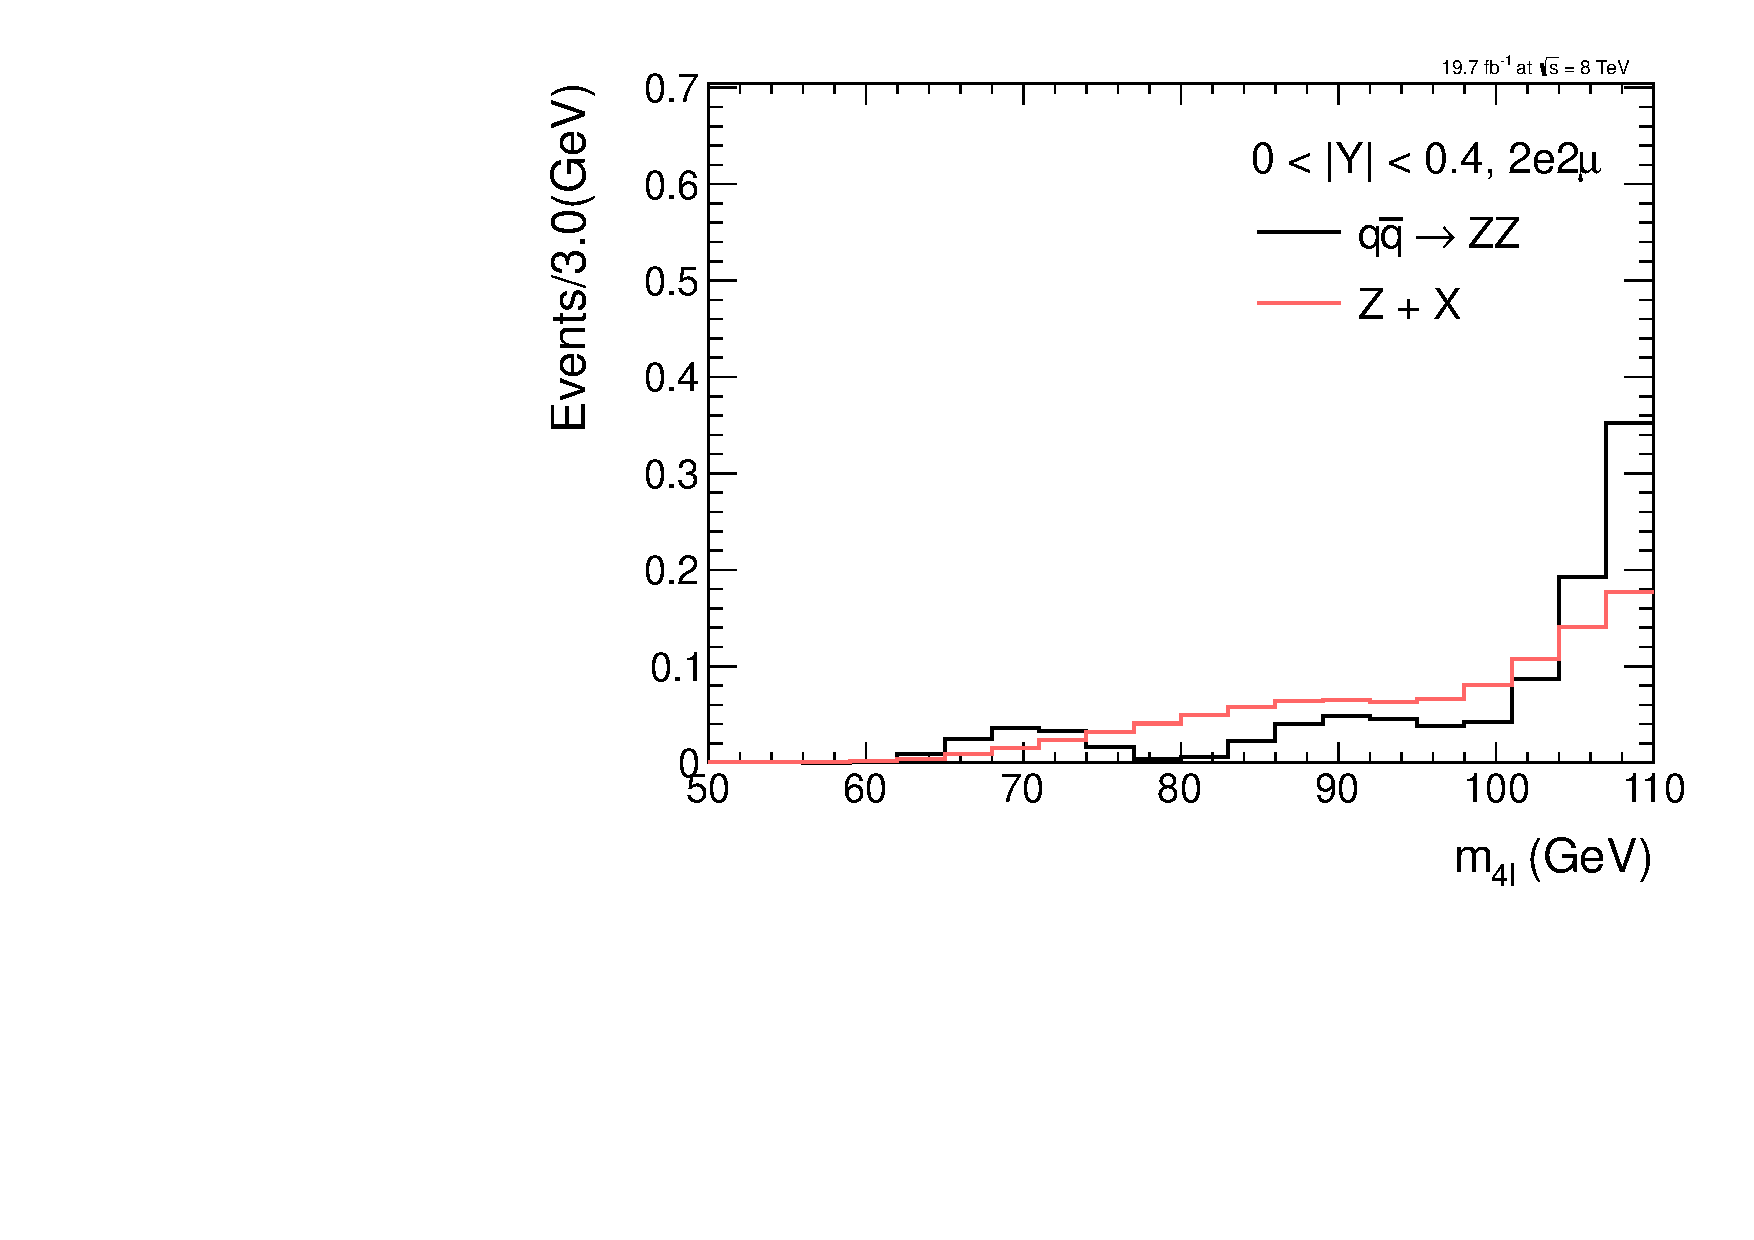
\includegraphics[width=0.32\textwidth,angle=0]{Appendix/figuresZ4l/XSTemplates_2e2mu_rapidity4l_recobin0_qqZZ_ZJetsCR.pdf}
      \label{fig:z4l_bkg-rapidity4l-qqZZ-ZX-2e2mu:a}
    }    
    \subfigure[$0.0 < |y(4\ell)| < 0.4$]{
      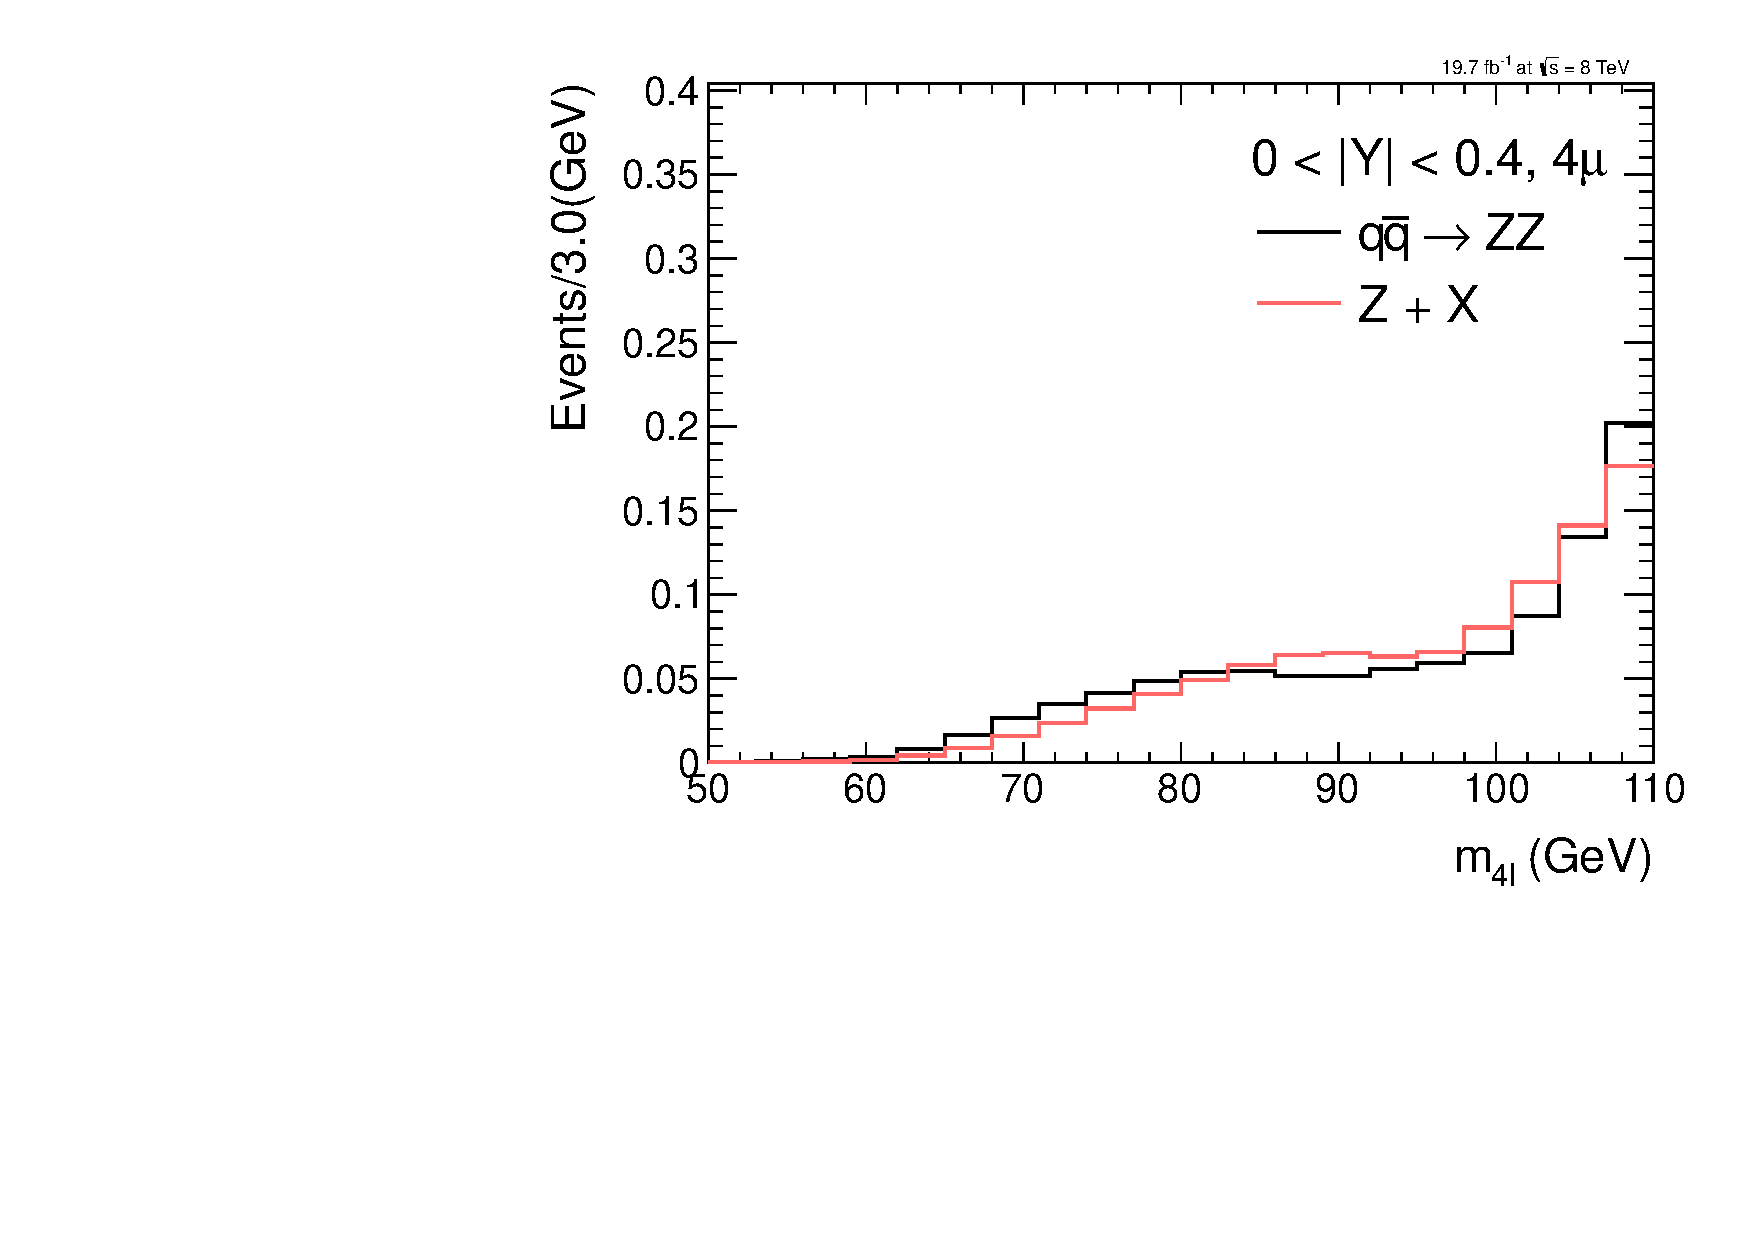
\includegraphics[width=0.32\textwidth,angle=0]{Appendix/figuresZ4l/XSTemplates_4mu_rapidity4l_recobin0_qqZZ_ZJetsCR.pdf}
      \label{fig:z4l_bkg-rapidity4l-qqZZ-ZX-4mu:a}
    }    
    \subfigure[$0.0 < |y(4\ell)| < 0.4$]{
      \includegraphics[width=0.32\textwidth,angle=0]{Appendix/figuresZ4l/XSTemplates_4e_rapidity4l_recobin0_qqZZ_ZJetsCR.pdf}
      \label{fig:z4l_bkg-rapidity4l-qqZZ-ZX-4e:a}
    }    \\

    \subfigure[$0.4 < |y(4\ell)| < 0.8$]{
      \includegraphics[width=0.32\textwidth,angle=0]{Appendix/figuresZ4l/XSTemplates_2e2mu_rapidity4l_recobin1_qqZZ_ZJetsCR.pdf}
      \label{fig:z4l_bkg-rapidity4l-qqZZ-ZX-2e2mu:b}
    }
    \subfigure[$0.4 < |y(4\ell)| < 0.8$]{
      \includegraphics[width=0.32\textwidth,angle=0]{Appendix/figuresZ4l/XSTemplates_4mu_rapidity4l_recobin1_qqZZ_ZJetsCR.pdf}
      \label{fig:z4l_bkg-rapidity4l-qqZZ-ZX-4mu:b}
    } 
    \subfigure[$0.4 < |y(4\ell)| < 0.8$]{
      \includegraphics[width=0.32\textwidth,angle=0]{Appendix/figuresZ4l/XSTemplates_4e_rapidity4l_recobin1_qqZZ_ZJetsCR.pdf}
      \label{fig:z4l_bkg-rapidity4l-qqZZ-ZX-4e:b}
    } \\
    
    \subfigure[$0.8 < |y(4\ell)| < 1.2$]{
      \includegraphics[width=0.32\textwidth,angle=0]{Appendix/figuresZ4l/XSTemplates_2e2mu_rapidity4l_recobin2_qqZZ_ZJetsCR.pdf}
      \label{fig:z4l_bkg-rapidity4l-qqZZ-ZX-2e2mu:c}
    }
    \subfigure[$0.8 < |y(4\ell)| < 1.2$]{
      \includegraphics[width=0.32\textwidth,angle=0]{Appendix/figuresZ4l/XSTemplates_4mu_rapidity4l_recobin2_qqZZ_ZJetsCR.pdf}
      \label{fig:z4l_bkg-rapidity4l-qqZZ-ZX-4mu:c}
    }
    \subfigure[$0.8 < |y(4\ell)| < 1.2$]{
      \includegraphics[width=0.32\textwidth,angle=0]{Appendix/figuresZ4l/XSTemplates_4e_rapidity4l_recobin2_qqZZ_ZJetsCR.pdf}
      \label{fig:z4l_bkg-rapidity4l-qqZZ-ZX-4e:c}
    } \\
    
    \subfigure[$1.2 < |y(4\ell)| < 2.4$]{
      \includegraphics[width=0.32\textwidth,angle=0]{Appendix/figuresZ4l/XSTemplates_2e2mu_rapidity4l_recobin3_qqZZ_ZJetsCR.pdf}
      \label{fig:z4l_bkg-rapidity4l-qqZZ-ZX-2e2mu:d}
    }
    \subfigure[$1.2 < |y(4\ell)| < 2.4$]{
      \includegraphics[width=0.32\textwidth,angle=0]{Appendix/figuresZ4l/XSTemplates_4mu_rapidity4l_recobin3_qqZZ_ZJetsCR.pdf}
      \label{fig:z4l_bkg-rapidity4l-qqZZ-ZX-4mu:d}
    }
    \subfigure[$1.2 < |y(4\ell)| < 2.4$]{
      \includegraphics[width=0.32\textwidth,angle=0]{Appendix/figuresZ4l/XSTemplates_4e_rapidity4l_recobin3_qqZZ_ZJetsCR.pdf}
      \label{fig:z4l_bkg-rapidity4l-qqZZ-ZX-4e:d}
    } \\
    
    \caption{ Distributions of m($4\ell$) for the $qq \rightarrow \mathrm{ZZ}$ and Z+X backgrounds in different bins of $|y(4\ell)|$ 
for Z$\to$4l measurements    
for three final states: $2e2\mu$(left), $4\mu$(middle) and $4e$(right).}
  \label{fig:z4l_bkg-rapidity4l-qqZZ-ZX}
  
 \end{center}
\end{figure} 

 \clearpage
 
 \begin{figure}[!ht]
  \begin{center}
  
    \subfigure[$0.0 < |y(4\ell)| < 0.4$]{
      \includegraphics[width=0.32\textwidth,angle=0]{Appendix/figuresZ4l/XSTemplates_2e2mu_rapidity4l_recobin0_qqZZ_ggZZ.pdf}
      \label{fig:z4l_bkg-rapidity4l-qqZZ-ggZZ-2e2mu:a}
    }    
    \subfigure[$0.0 < |y(4\ell)| < 0.4$]{
      \includegraphics[width=0.32\textwidth,angle=0]{Appendix/figuresZ4l/XSTemplates_4mu_rapidity4l_recobin0_qqZZ_ggZZ.pdf}
      \label{fig:z4l_bkg-rapidity4l-qqZZ-ggZZ-4mu:a}
    }    
    \subfigure[$0.0 < |y(4\ell)| < 0.4$]{
      \includegraphics[width=0.32\textwidth,angle=0]{Appendix/figuresZ4l/XSTemplates_4e_rapidity4l_recobin0_qqZZ_ggZZ.pdf}
      \label{fig:z4l_bkg-rapidity4l-qqZZ-ggZZ-4e:a}
    }    \\

    \subfigure[$0.4 < |y(4\ell)| < 0.8$]{
      \includegraphics[width=0.32\textwidth,angle=0]{Appendix/figuresZ4l/XSTemplates_2e2mu_rapidity4l_recobin1_qqZZ_ggZZ.pdf}
      \label{fig:z4l_bkg-rapidity4l-qqZZ-ggZZ-2e2mu:b}
    }
    \subfigure[$0.4 < |y(4\ell)| < 0.8$]{
      \includegraphics[width=0.32\textwidth,angle=0]{Appendix/figuresZ4l/XSTemplates_4mu_rapidity4l_recobin1_qqZZ_ggZZ.pdf}
      \label{fig:z4l_bkg-rapidity4l-qqZZ-ggZZ-4mu:b}
    } 
    \subfigure[$0.4 < |y(4\ell)| < 0.8$]{
      \includegraphics[width=0.32\textwidth,angle=0]{Appendix/figuresZ4l/XSTemplates_4e_rapidity4l_recobin1_qqZZ_ggZZ.pdf}
      \label{fig:z4l_bkg-rapidity4l-qqZZ-ggZZ-4e:b}
    } \\
    
    \subfigure[$0.8 < |y(4\ell)| < 1.2$]{
      \includegraphics[width=0.32\textwidth,angle=0]{Appendix/figuresZ4l/XSTemplates_2e2mu_rapidity4l_recobin2_qqZZ_ggZZ.pdf}
      \label{fig:z4l_bkg-rapidity4l-qqZZ-ggZZ-2e2mu:c}
    }
    \subfigure[$0.8 < |y(4\ell)| < 1.2$]{
      \includegraphics[width=0.32\textwidth,angle=0]{Appendix/figuresZ4l/XSTemplates_4mu_rapidity4l_recobin2_qqZZ_ggZZ.pdf}
      \label{fig:z4l_bkg-rapidity4l-qqZZ-ggZZ-4mu:c}
    }
    \subfigure[$0.8 < |y(4\ell)| < 1.2$]{
      \includegraphics[width=0.32\textwidth,angle=0]{Appendix/figuresZ4l/XSTemplates_4e_rapidity4l_recobin2_qqZZ_ggZZ.pdf}
      \label{fig:z4l_bkg-rapidity4l-qqZZ-ggZZ-4e:c}
    } \\
    
    \subfigure[$1.2 < |y(4\ell)| < 2.4$]{
      \includegraphics[width=0.32\textwidth,angle=0]{Appendix/figuresZ4l/XSTemplates_2e2mu_rapidity4l_recobin3_qqZZ_ggZZ.pdf}
      \label{fig:z4l_bkg-rapidity4l-qqZZ-ggZZ-2e2mu:d}
    }
    \subfigure[$1.2 < |y(4\ell)| < 2.4$]{
      \includegraphics[width=0.32\textwidth,angle=0]{Appendix/figuresZ4l/XSTemplates_4mu_rapidity4l_recobin3_qqZZ_ggZZ.pdf}
      \label{fig:z4l_bkg-rapidity4l-qqZZ-ggZZ-4mu:d}
    }
    \subfigure[$1.2 < |y(4\ell)| < 2.4$]{
      \includegraphics[width=0.32\textwidth,angle=0]{Appendix/figuresZ4l/XSTemplates_4e_rapidity4l_recobin3_qqZZ_ggZZ.pdf}
      \label{fig:z4l_bkg-rapidity4l-qqZZ-ggZZ-4e:d}
    } \\
    
    \caption{ Distributions of m($4\ell$) for the $qq \rightarrow \mathrm{ZZ}$ and $gg \rightarrow \mathrm{ZZ}$ backgrounds 
    in different bins of $|y(4\ell)|$ 
for Z$\to$4l measurements
for three final states: $2e2\mu$(left), $4\mu$(middle) and $4e$(right).}
  \label{fig:z4l_bkg-rapidity4l-qqZZ-ggZZ}
  
 \end{center}
\end{figure} 

\clearpage


\subsection{Background shapes in bins of $|\cos \theta^{*}|$ }

\begin{figure}[!ht]
  \begin{center}
  
    \subfigure[$0.0 < |\cos \theta^{*}| < 0.25$]{
      \includegraphics[width=0.32\textwidth,angle=0]{Appendix/figuresZ4l/XSTemplates_2e2mu_cosThetaStar_recobin0_qqZZ_ZJetsCR.pdf}
      \label{fig:z4l_bkg-cosThetaStar-qqZZ-ZX-2e2mu:a}
    }    
    \subfigure[$0.0 < |\cos \theta^{*}| < 0.25$]{
      \includegraphics[width=0.32\textwidth,angle=0]{Appendix/figuresZ4l/XSTemplates_4mu_cosThetaStar_recobin0_qqZZ_ZJetsCR.pdf}
      \label{fig:z4l_bkg-cosThetaStar-qqZZ-ZX-4mu:a}
    }    
    \subfigure[$0.0 < |\cos \theta^{*}| < 0.25$]{
      \includegraphics[width=0.32\textwidth,angle=0]{Appendix/figuresZ4l/XSTemplates_4e_cosThetaStar_recobin0_qqZZ_ZJetsCR.pdf}
      \label{fig:z4l_bkg-cosThetaStar-qqZZ-ZX-4e:a}
    }    \\

    \subfigure[$0.25 < |\cos \theta^{*}| < 0.50$]{
      \includegraphics[width=0.32\textwidth,angle=0]{Appendix/figuresZ4l/XSTemplates_2e2mu_cosThetaStar_recobin1_qqZZ_ZJetsCR.pdf}
      \label{fig:z4l_bkg-cosThetaStar-qqZZ-ZX-2e2mu:b}
    }
    \subfigure[$0.25 < |\cos \theta^{*}| < 0.50$]{
      \includegraphics[width=0.32\textwidth,angle=0]{Appendix/figuresZ4l/XSTemplates_4mu_cosThetaStar_recobin1_qqZZ_ZJetsCR.pdf}
      \label{fig:z4l_bkg-cosThetaStar-qqZZ-ZX-4mu:b}
    } 
    \subfigure[$0.25 < |\cos \theta^{*}| < 0.50$]{
      \includegraphics[width=0.32\textwidth,angle=0]{Appendix/figuresZ4l/XSTemplates_4e_cosThetaStar_recobin1_qqZZ_ZJetsCR.pdf}
      \label{fig:z4l_bkg-cosThetaStar-qqZZ-ZX-4e:b}
    } \\
    
    \subfigure[$0.50 < |\cos \theta^{*}| < 0.75$]{
      \includegraphics[width=0.32\textwidth,angle=0]{Appendix/figuresZ4l/XSTemplates_2e2mu_cosThetaStar_recobin2_qqZZ_ZJetsCR.pdf}
      \label{fig:z4l_bkg-cosThetaStar-qqZZ-ZX-2e2mu:c}
    }
    \subfigure[$0.50 < |\cos \theta^{*}| < 0.75$]{
      \includegraphics[width=0.32\textwidth,angle=0]{Appendix/figuresZ4l/XSTemplates_4mu_cosThetaStar_recobin2_qqZZ_ZJetsCR.pdf}
      \label{fig:z4l_bkg-cosThetaStar-qqZZ-ZX-4mu:c}
    }
    \subfigure[$0.50 < |\cos \theta^{*}| < 0.75$]{
      \includegraphics[width=0.32\textwidth,angle=0]{Appendix/figuresZ4l/XSTemplates_4e_cosThetaStar_recobin2_qqZZ_ZJetsCR.pdf}
      \label{fig:z4l_bkg-cosThetaStar-qqZZ-ZX-4e:c}
    } \\
    
    \subfigure[$0.75 < |\cos \theta^{*}| < 1.0$]{
      \includegraphics[width=0.32\textwidth,angle=0]{Appendix/figuresZ4l/XSTemplates_2e2mu_cosThetaStar_recobin3_qqZZ_ZJetsCR.pdf}
      \label{fig:z4l_bkg-cosThetaStar-qqZZ-ZX-2e2mu:d}
    }
    \subfigure[$0.75 < |\cos \theta^{*}| < 1.0$]{
      \includegraphics[width=0.32\textwidth,angle=0]{Appendix/figuresZ4l/XSTemplates_4mu_cosThetaStar_recobin3_qqZZ_ZJetsCR.pdf}
      \label{fig:z4l_bkg-cosThetaStar-qqZZ-ZX-4mu:d}
    }
    \subfigure[$0.75 < |\cos \theta^{*}| < 1.0$]{
      \includegraphics[width=0.32\textwidth,angle=0]{Appendix/figuresZ4l/XSTemplates_4e_cosThetaStar_recobin3_qqZZ_ZJetsCR.pdf}
      \label{fig:z4l_bkg-cosThetaStar-qqZZ-ZX-4e:d}
    } \\
    
    \caption{ Distributions of m($4\ell$) for the $qq \rightarrow \mathrm{ZZ}$ and Z+X backgrounds in different bins of  $|\cos \theta^{*}|$
for Z$\to$4l measurements 
   for three final states: $2e2\mu$(left), $4\mu$(middle) and $4e$(right).}
  \label{fig:z4l_bkg-cosThetaStar-qqZZ-ZX}
  
 \end{center}
\end{figure} 

 \clearpage
 
 \begin{figure}[!ht]
  \begin{center}
  
    \subfigure[$0.0 < |\cos \theta^{*}| < 0.25$]{
      \includegraphics[width=0.32\textwidth,angle=0]{Appendix/figuresZ4l/XSTemplates_2e2mu_cosThetaStar_recobin0_qqZZ_ggZZ.pdf}
      \label{fig:z4l_bkg-cosThetaStar-qqZZ-ggZZ-2e2mu:a}
    }    
    \subfigure[$0.0 < |\cos \theta^{*}| < 0.25$]{
      \includegraphics[width=0.32\textwidth,angle=0]{Appendix/figuresZ4l/XSTemplates_4mu_cosThetaStar_recobin0_qqZZ_ggZZ.pdf}
      \label{fig:z4l_bkg-cosThetaStar-qqZZ-ggZZ-4mu:a}
    }    
    \subfigure[$0.0 < |\cos \theta^{*}| < 0.25$]{
      \includegraphics[width=0.32\textwidth,angle=0]{Appendix/figuresZ4l/XSTemplates_4e_cosThetaStar_recobin0_qqZZ_ggZZ.pdf}
      \label{fig:z4l_bkg-cosThetaStar-qqZZ-ggZZ-4e:a}
    }    \\

    \subfigure[$0.25 < |\cos \theta^{*}| < 0.50$]{
      \includegraphics[width=0.32\textwidth,angle=0]{Appendix/figuresZ4l/XSTemplates_2e2mu_cosThetaStar_recobin1_qqZZ_ggZZ.pdf}
      \label{fig:z4l_bkg-cosThetaStar-qqZZ-ggZZ-2e2mu:b}
    }
    \subfigure[$0.25 < |\cos \theta^{*}| < 0.50$]{
      \includegraphics[width=0.32\textwidth,angle=0]{Appendix/figuresZ4l/XSTemplates_4mu_cosThetaStar_recobin1_qqZZ_ggZZ.pdf}
      \label{fig:z4l_bkg-cosThetaStar-qqZZ-ggZZ-4mu:b}
    } 
    \subfigure[$0.25 < |\cos \theta^{*}| < 0.50$]{
      \includegraphics[width=0.32\textwidth,angle=0]{Appendix/figuresZ4l/XSTemplates_4e_cosThetaStar_recobin1_qqZZ_ggZZ.pdf}
      \label{fig:z4l_bkg-cosThetaStar-qqZZ-ggZZ-4e:b}
    } \\
    
    \subfigure[$0.50 < |\cos \theta^{*}| < 0.75$]{
      \includegraphics[width=0.32\textwidth,angle=0]{Appendix/figuresZ4l/XSTemplates_2e2mu_cosThetaStar_recobin2_qqZZ_ggZZ.pdf}
      \label{fig:z4l_bkg-cosThetaStar-qqZZ-ggZZ-2e2mu:c}
    }
    \subfigure[$0.50 < |\cos \theta^{*}| < 0.75$]{
      \includegraphics[width=0.32\textwidth,angle=0]{Appendix/figuresZ4l/XSTemplates_4mu_cosThetaStar_recobin2_qqZZ_ggZZ.pdf}
      \label{fig:z4l_bkg-cosThetaStar-qqZZ-ggZZ-4mu:c}
    }
    \subfigure[$0.50 < |\cos \theta^{*}| < 0.75$]{
      \includegraphics[width=0.32\textwidth,angle=0]{Appendix/figuresZ4l/XSTemplates_4e_cosThetaStar_recobin2_qqZZ_ggZZ.pdf}
      \label{fig:z4l_bkg-cosThetaStar-qqZZ-ggZZ-4e:c}
    } \\
    
    \subfigure[$0.75 < |\cos \theta^{*}| < 1.0$]{
      \includegraphics[width=0.32\textwidth,angle=0]{Appendix/figuresZ4l/XSTemplates_2e2mu_cosThetaStar_recobin3_qqZZ_ggZZ.pdf}
      \label{fig:z4l_bkg-cosThetaStar-qqZZ-ggZZ-2e2mu:d}
    }
    \subfigure[$0.75 < |\cos \theta^{*}| < 1.0$]{
      \includegraphics[width=0.32\textwidth,angle=0]{Appendix/figuresZ4l/XSTemplates_4mu_cosThetaStar_recobin3_qqZZ_ggZZ.pdf}
      \label{fig:z4l_bkg-cosThetaStar-qqZZ-ggZZ-4mu:d}
    }
    \subfigure[$0.75 < |\cos \theta^{*}| < 1.0$]{
      \includegraphics[width=0.32\textwidth,angle=0]{Appendix/figuresZ4l/XSTemplates_4e_cosThetaStar_recobin3_qqZZ_ggZZ.pdf}
      \label{fig:z4l_bkg-cosThetaStar-qqZZ-ggZZ-4e:d}
    } \\
    
    \caption{ Distributions of m($4\ell$) for the $qq \rightarrow \mathrm{ZZ}$ and $gg \rightarrow \mathrm{ZZ}$ backgrounds 
    in different bins of  $|\cos \theta^{*}|$ 
for Z$\to$4l measurements
for three final states: $2e2\mu$(left), $4\mu$(middle) and $4e$(right).}
  \label{fig:z4l_bkg-cosThetaStar-qqZZ-ggZZ}
  
 \end{center}
\end{figure} 

\clearpage


\subsection{Background shapes in bins of $N_{\rm jets}$ }

\begin{figure}[!ht]
  \begin{center}
  
    \subfigure[$\mathrm{N(jets)}=0$]{
      \includegraphics[width=0.32\textwidth,angle=0]{Appendix/figuresZ4l/XSTemplates_2e2mu_njets_reco_pt30_eta4p7_0_1_qqZZ_ZJetsCR.pdf}
      \label{fig:z4l_bkg-njets_reco_pt30_eta4p7-qqZZ-ZX-2e2mu:a}
    }    
    \subfigure[$\mathrm{N(jets)}=0$]{
      \includegraphics[width=0.32\textwidth,angle=0]{Appendix/figuresZ4l/XSTemplates_4mu_njets_reco_pt30_eta4p7_0_1_qqZZ_ZJetsCR.pdf}
      \label{fig:z4l_bkg-njets_reco_pt30_eta4p7-qqZZ-ZX-4mu:a}
    }    
    \subfigure[$\mathrm{N(jets)}=0$]{
      \includegraphics[width=0.32\textwidth,angle=0]{Appendix/figuresZ4l/XSTemplates_4e_njets_reco_pt30_eta4p7_0_1_qqZZ_ZJetsCR.pdf}
      \label{fig:z4l_bkg-njets_reco_pt30_eta4p7-qqZZ-ZX-4e:a}
    }    \\

    \subfigure[$\mathrm{N(jets)}=1$]{
      \includegraphics[width=0.32\textwidth,angle=0]{Appendix/figuresZ4l/XSTemplates_2e2mu_njets_reco_pt30_eta4p7_1_2_qqZZ_ZJetsCR.pdf}
      \label{fig:z4l_bkg-njets_reco_pt30_eta4p7-qqZZ-ZX-2e2mu:b}
    }
    \subfigure[$\mathrm{N(jets)}=1$]{
      \includegraphics[width=0.32\textwidth,angle=0]{Appendix/figuresZ4l/XSTemplates_4mu_njets_reco_pt30_eta4p7_1_2_qqZZ_ZJetsCR.pdf}
      \label{fig:z4l_bkg-njets_reco_pt30_eta4p7-qqZZ-ZX-4mu:b}
    } 
    \subfigure[$\mathrm{N(jets)}=1$]{
      \includegraphics[width=0.32\textwidth,angle=0]{Appendix/figuresZ4l/XSTemplates_4e_njets_reco_pt30_eta4p7_1_2_qqZZ_ZJetsCR.pdf}
      \label{fig:z4l_bkg-njets_reco_pt30_eta4p7-qqZZ-ZX-4e:b}
    } \\
    
    \subfigure[$\mathrm{N(jets)}=2$]{
      \includegraphics[width=0.32\textwidth,angle=0]{Appendix/figuresZ4l/XSTemplates_2e2mu_njets_reco_pt30_eta4p7_2_3_qqZZ_ZJetsCR.pdf}
      \label{fig:z4l_bkg-njets_reco_pt30_eta4p7-qqZZ-ZX-2e2mu:c}
    }
    \subfigure[$\mathrm{N(jets)}=2$]{
      \includegraphics[width=0.32\textwidth,angle=0]{Appendix/figuresZ4l/XSTemplates_4mu_njets_reco_pt30_eta4p7_2_3_qqZZ_ZJetsCR.pdf}
      \label{fig:z4l_bkg-njets_reco_pt30_eta4p7-qqZZ-ZX-4mu:c}
    }
    \subfigure[$\mathrm{N(jets)}=2$]{
      \includegraphics[width=0.32\textwidth,angle=0]{Appendix/figuresZ4l/XSTemplates_4e_njets_reco_pt30_eta4p7_2_3_qqZZ_ZJetsCR.pdf}
      \label{fig:z4l_bkg-njets_reco_pt30_eta4p7-qqZZ-ZX-4e:c}
    } \\
    
    \subfigure[$\mathrm{N(jets)} \geq 3$]{
      \includegraphics[width=0.32\textwidth,angle=0]{Appendix/figuresZ4l/XSTemplates_2e2mu_njets_reco_pt30_eta4p7_3_10_qqZZ_ZJetsCR.pdf}
      \label{fig:z4l_bkg-njets_reco_pt30_eta4p7-qqZZ-ZX-2e2mu:d}
    }
    \subfigure[$\mathrm{N(jets)} \geq 3$]{
      \includegraphics[width=0.32\textwidth,angle=0]{Appendix/figuresZ4l/XSTemplates_4mu_njets_reco_pt30_eta4p7_3_10_qqZZ_ZJetsCR.pdf}
      \label{fig:z4l_bkg-njets_reco_pt30_eta4p7-qqZZ-ZX-4mu:d}
    }
    \subfigure[$\mathrm{N(jets)} \geq 3$]{
      \includegraphics[width=0.32\textwidth,angle=0]{Appendix/figuresZ4l/XSTemplates_4e_njets_reco_pt30_eta4p7_3_10_qqZZ_ZJetsCR.pdf}
      \label{fig:z4l_bkg-njets_reco_pt30_eta4p7-qqZZ-ZX-4e:d}
    } \\
    
    \caption{ Distributions of m($4\ell$) for the $qq \rightarrow \mathrm{ZZ}$ and Z+X backgrounds in different bins of $N_{\rm jets}$
for Z$\to$4l measurements    
for three final states: $2e2\mu$(left), $4\mu$(middle) and $4e$(right).}
  \label{fig:z4l_bkg-njets_reco_pt30_eta4p7-qqZZ-ZX}
  
 \end{center}
\end{figure} 

 \clearpage
 
 \begin{figure}[!ht]
  \begin{center}
  
    \subfigure[$\mathrm{N(jets)}=0$]{
      \includegraphics[width=0.32\textwidth,angle=0]{Appendix/figuresZ4l/XSTemplates_2e2mu_njets_reco_pt30_eta4p7_0_1_qqZZ_ggZZ.pdf}
      \label{fig:z4l_bkg-njets_reco_pt30_eta4p7-qqZZ-ggZZ-2e2mu:a}
    }    
    \subfigure[$\mathrm{N(jets)}=0$]{
      \includegraphics[width=0.32\textwidth,angle=0]{Appendix/figuresZ4l/XSTemplates_4mu_njets_reco_pt30_eta4p7_0_1_qqZZ_ggZZ.pdf}
      \label{fig:z4l_bkg-njets_reco_pt30_eta4p7-qqZZ-ggZZ-4mu:a}
    }    
    \subfigure[$\mathrm{N(jets)}=0$]{
      \includegraphics[width=0.32\textwidth,angle=0]{Appendix/figuresZ4l/XSTemplates_4e_njets_reco_pt30_eta4p7_0_1_qqZZ_ggZZ.pdf}
      \label{fig:z4l_bkg-njets_reco_pt30_eta4p7-qqZZ-ggZZ-4e:a}
    }    \\

    \subfigure[$\mathrm{N(jets)}=1$]{
      \includegraphics[width=0.32\textwidth,angle=0]{Appendix/figuresZ4l/XSTemplates_2e2mu_njets_reco_pt30_eta4p7_1_2_qqZZ_ggZZ.pdf}
      \label{fig:z4l_bkg-njets_reco_pt30_eta4p7-qqZZ-ggZZ-2e2mu:b}
    }
    \subfigure[$\mathrm{N(jets)}=1$]{
      \includegraphics[width=0.32\textwidth,angle=0]{Appendix/figuresZ4l/XSTemplates_4mu_njets_reco_pt30_eta4p7_1_2_qqZZ_ggZZ.pdf}
      \label{fig:z4l_bkg-njets_reco_pt30_eta4p7-qqZZ-ggZZ-4mu:b}
    } 
    \subfigure[$\mathrm{N(jets)}=1$]{
      \includegraphics[width=0.32\textwidth,angle=0]{Appendix/figuresZ4l/XSTemplates_4e_njets_reco_pt30_eta4p7_1_2_qqZZ_ggZZ.pdf}
      \label{fig:z4l_bkg-njets_reco_pt30_eta4p7-qqZZ-ggZZ-4e:b}
    } \\
    
    \subfigure[$\mathrm{N(jets)}=2$]{
      \includegraphics[width=0.32\textwidth,angle=0]{Appendix/figuresZ4l/XSTemplates_2e2mu_njets_reco_pt30_eta4p7_2_3_qqZZ_ggZZ.pdf}
      \label{fig:z4l_bkg-njets_reco_pt30_eta4p7-qqZZ-ggZZ-2e2mu:c}
    }
    \subfigure[$\mathrm{N(jets)}=2$]{
      \includegraphics[width=0.32\textwidth,angle=0]{Appendix/figuresZ4l/XSTemplates_4mu_njets_reco_pt30_eta4p7_2_3_qqZZ_ggZZ.pdf}
      \label{fig:z4l_bkg-njets_reco_pt30_eta4p7-qqZZ-ggZZ-4mu:c}
    }
    \subfigure[$\mathrm{N(jets)}=2$]{
      \includegraphics[width=0.32\textwidth,angle=0]{Appendix/figuresZ4l/XSTemplates_4e_njets_reco_pt30_eta4p7_2_3_qqZZ_ggZZ.pdf}
      \label{fig:z4l_bkg-njets_reco_pt30_eta4p7-qqZZ-ggZZ-4e:c}
    } \\
    
    \subfigure[$\mathrm{N(jets)} \geq 3$]{
      \includegraphics[width=0.32\textwidth,angle=0]{Appendix/figuresZ4l/XSTemplates_2e2mu_njets_reco_pt30_eta4p7_3_10_qqZZ_ggZZ.pdf}
      \label{fig:z4l_bkg-njets_reco_pt30_eta4p7-qqZZ-ggZZ-2e2mu:d}
    }
    \subfigure[$\mathrm{N(jets)} \geq 3$]{
      \includegraphics[width=0.32\textwidth,angle=0]{Appendix/figuresZ4l/XSTemplates_4mu_njets_reco_pt30_eta4p7_3_10_qqZZ_ggZZ.pdf}
      \label{fig:z4l_bkg-njets_reco_pt30_eta4p7-qqZZ-ggZZ-4mu:d}
    }
    \subfigure[$\mathrm{N(jets)} \geq 3$]{
      \includegraphics[width=0.32\textwidth,angle=0]{Appendix/figuresZ4l/XSTemplates_4e_njets_reco_pt30_eta4p7_3_10_qqZZ_ggZZ.pdf}
      \label{fig:z4l_bkg-njets_reco_pt30_eta4p7-qqZZ-ggZZ-4e:d}
    } \\
    
    \caption{ Distributions of m($4\ell$) for the $qq \rightarrow \mathrm{ZZ}$ and $gg \rightarrow \mathrm{ZZ}$ backgrounds 
    in different bins of $N_{\rm jets}$ 
for Z$\to$4l measurements
for three final states: $2e2\mu$(left), $4\mu$(middle) and $4e$(right).}
  \label{fig:z4l_bkg-njets_reco_pt30_eta4p7-qqZZ-ggZZ}
  
 \end{center}
\end{figure} 

\clearpage
